\chapter{Experimenting with Radar-based Gestures}
\label{chap:radar-experiments}

In this chapter, we attempt to validate the radar processing pipeline designed in Chapter~\ref{chap:radar-challenges} through experimentation and address three of the five research questions defined in Section~\ref{sec:introduction:research:research-questions}: 
\begin{itemize}
    \item [RQ2] \textit{What is the performance of radar sensors for mid-air gesture recognition?}
    \item [RQ3] \textit{What types of gesture-based applications would benefit from radar sensors?}
    \item [RQ4] \textit{How can we foster collaboration between researchers and practitioners working on (radar) gesture recognition?}
\end{itemize}
To this end, we collected three datasets that emulate different contexts (environment, sensor(s)) and feature a wide variety of gestures. These contributions are illustrated in \fig~\ref{fig:radar-experiments:graphical-summary}. The rest of the chapter is organized as follows.
%
Section~\ref{sec:radar-experiments:data-collection} provides information about our data collection, including the three sensors that we employed, the three datasets, and the pre-processing applied to radar data.
%
A first experiment is conducted in Section~\ref{sec:radar-experiments:sensors}, in which the performance of three different sensors (one vision-based and two radar-based) is compared on a dataset of 16 gestures.
%
A second experiment is carried out in Section~\ref{sec:radar-experiments:gesture-subsets}, in which the performance of the Walabot is evaluated in user-dependent, user-independent, and mixed scenarios on an extended dataset of 20 gestures and well-differentiated subsets of gestures.
%
A third experiment is conducted in Section~\ref{sec:radar-experiments:through-materials} to analyze the impact of occlusion by three different types of materials (wood, PVC, and glass) on the Walabot and confirm whether our pre-processing pipeline can successfully normalize its signal for accurate gesture recognition.
%
Section~\ref{sec:radar-experiments:discussion} then discusses the results of these three experiments and their implications on the design of radar-based gesture recognition.
%
Finally, Section~\ref{sec:radar-experiments:conclusion} concludes this chapter.

\begin{figure}
    \centering
    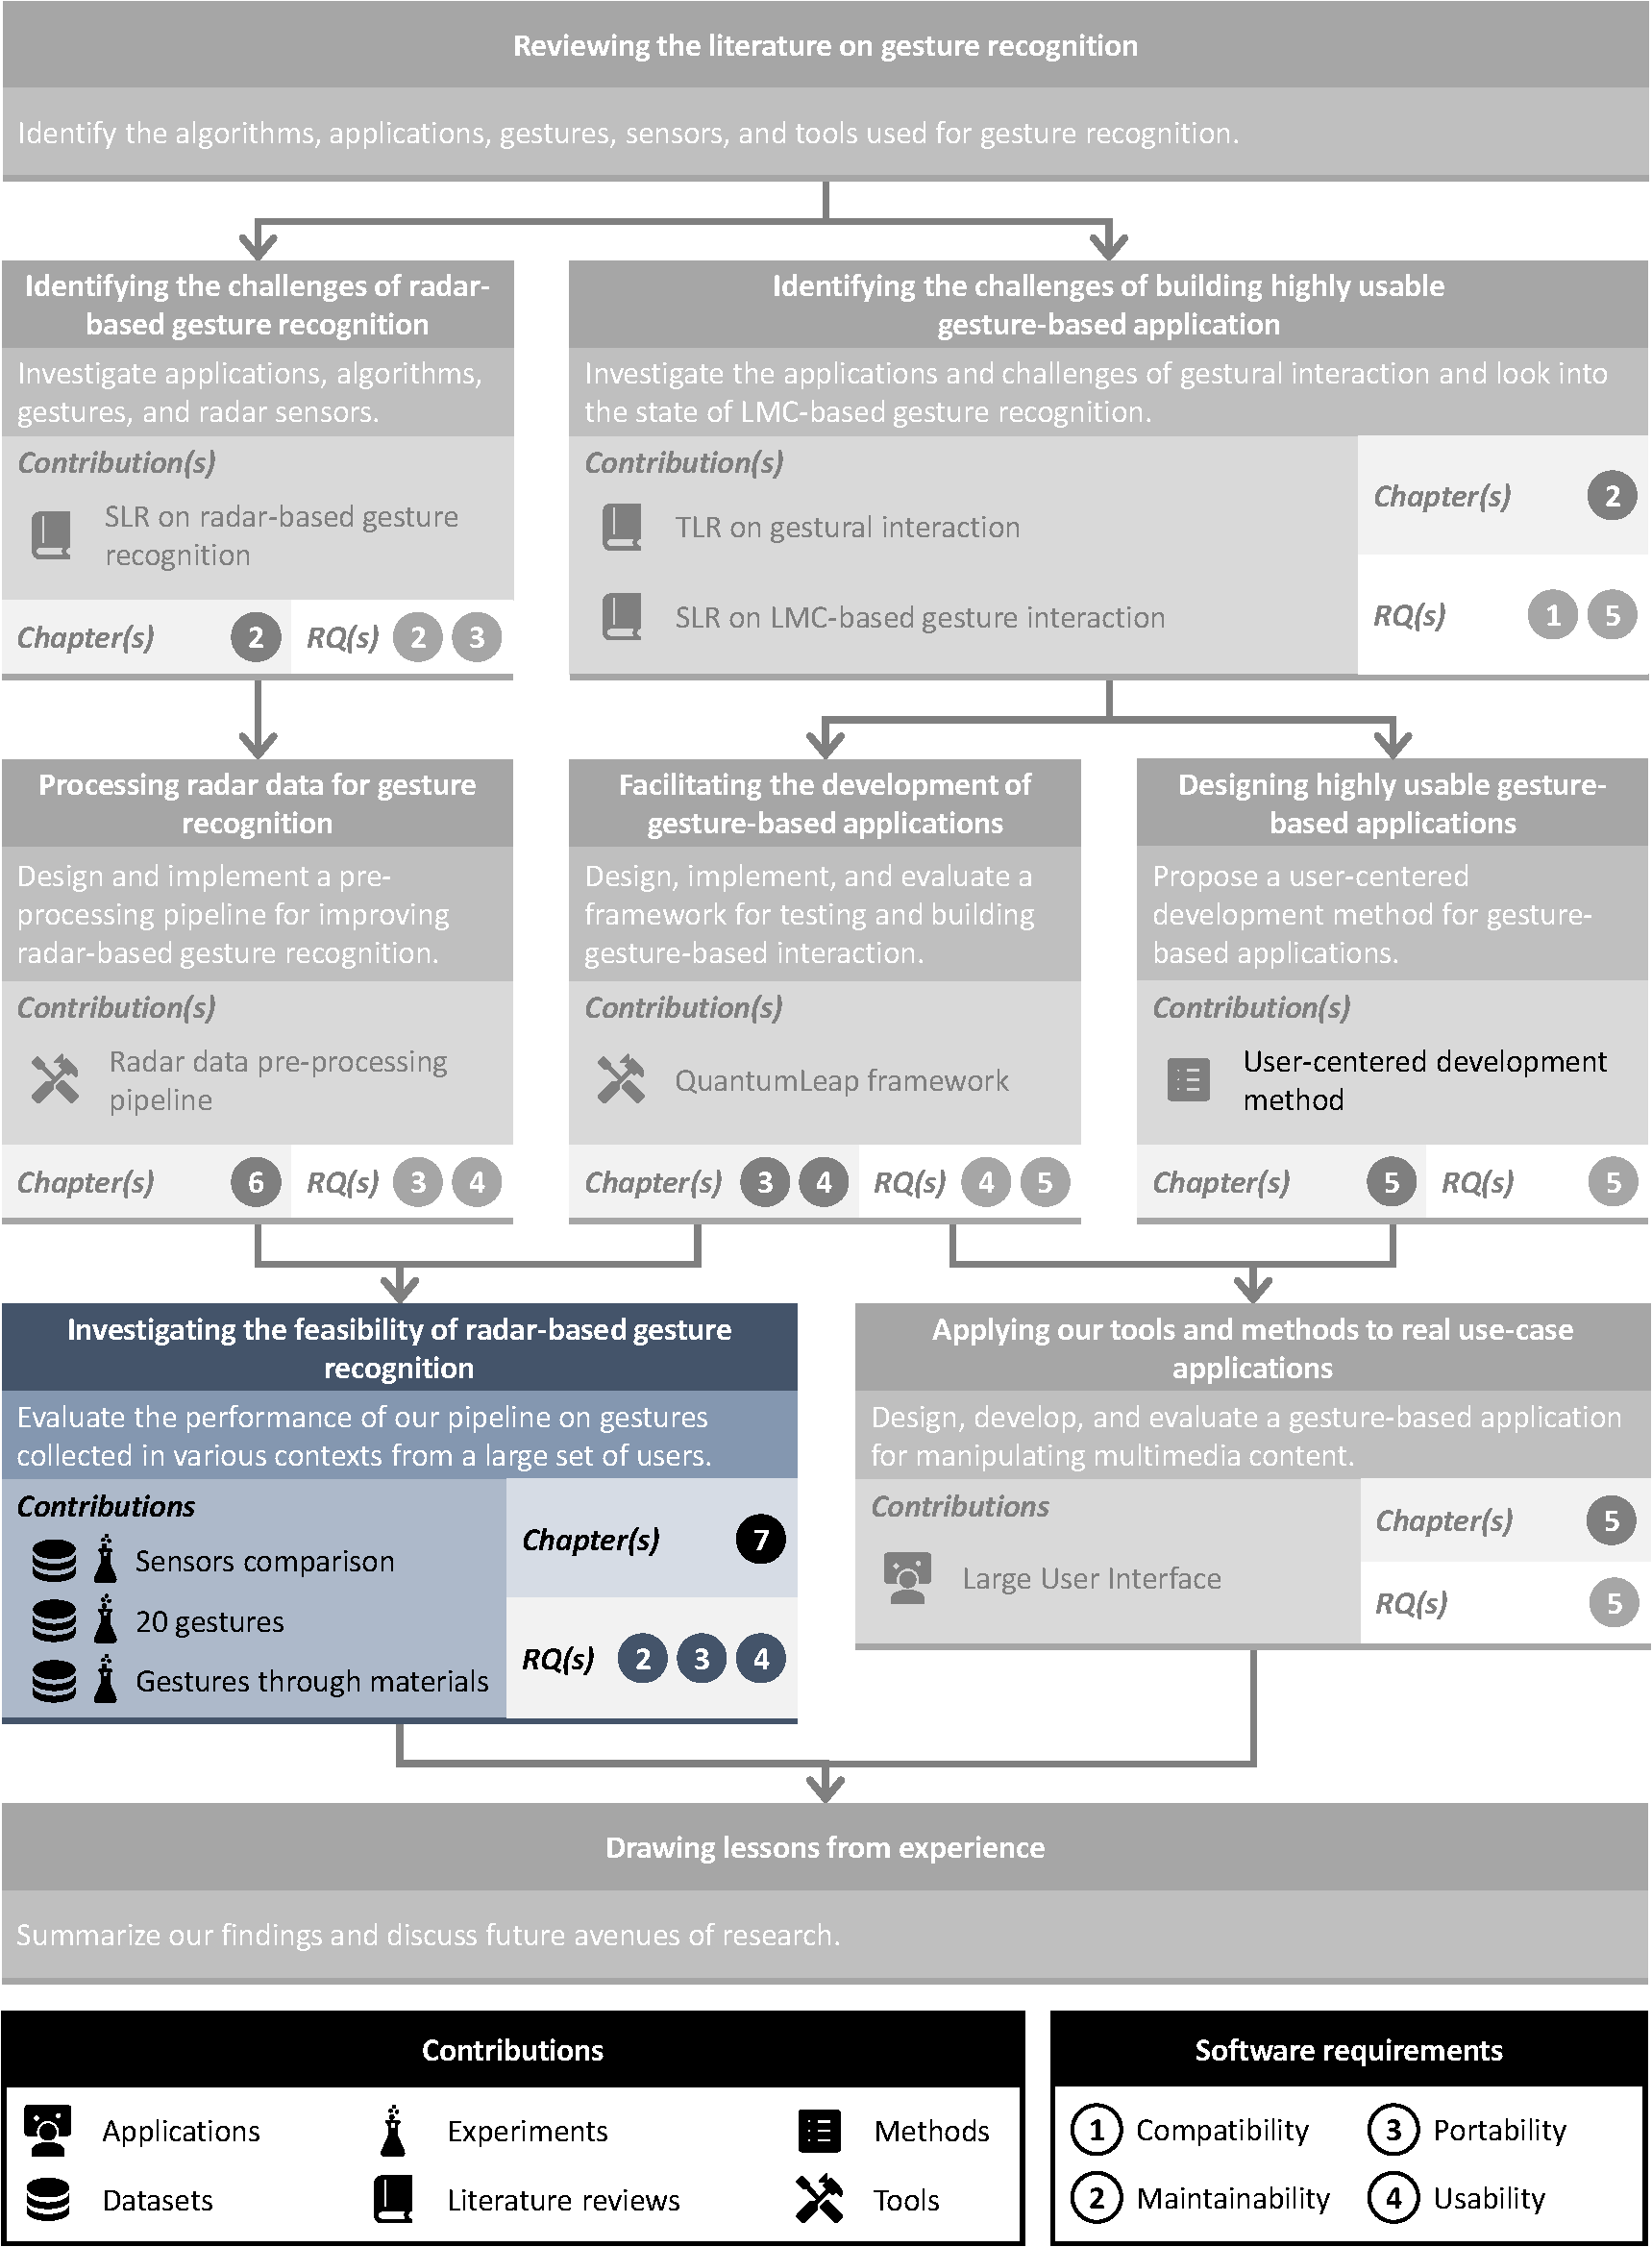
\includegraphics[width=\linewidth]{Figures/RadarExperiments/graphical-summary-radar-experiments.pdf}
    \vspace{-18pt}
    \caption{Main contributions of this chapter.}
    \label{fig:radar-experiments:graphical-summary}
  \end{figure}

\paragraph{Publications.} This chapter is based on three papers published in the IUI 2022 conference proceedings (Best paper award)~\cite{Sluyters:2022:IUI}, ACM TiiS journal~\cite{Sluyters:2023}, and IEEE Access journal~\cite{Sluyters:2024}.
% IUI2024?}

\paragraph{Resources.} The datasets, testing configurations, and results from the experiments conducted in this chapter are available on OSF at \url{https://osf.io/q43j8/?view_only=20b39a8a3d994ae4bd9ce52bfa2ded28}.


%================================================================================%
\section{Data Collection} \label{sec:radar-experiments:data-collection}
This section provides information about our data collection, consisting of three different datasets collected using three different sensors. 
Section~\ref{sec:radar-experiments:data-collection:sensors} describes the three sensors while Section~\ref{sec:radar-experiments:data-collection:datasets} goes over the three datasets, including their gestures and recording procedure.
Section~\ref{sec:radar-experiments:data-collection:pre-processing} provides details on the pre-processing applied to each gesture based on the pipeline proposed in Chapter~\ref{chap:radar-challenges}.

%--------------------------------------------------------------------------------%
\subsection{Sensors} \label{sec:radar-experiments:data-collection:sensors}
This section describes the three sensors that we used for data collection, including a vision-based sensor (the LMC) and two radar sensors (a Walabot and a custom horn antenna).

\begin{figure}[!b]
    \centering
    \begin{subfigure}{.46\linewidth}
        \centering
        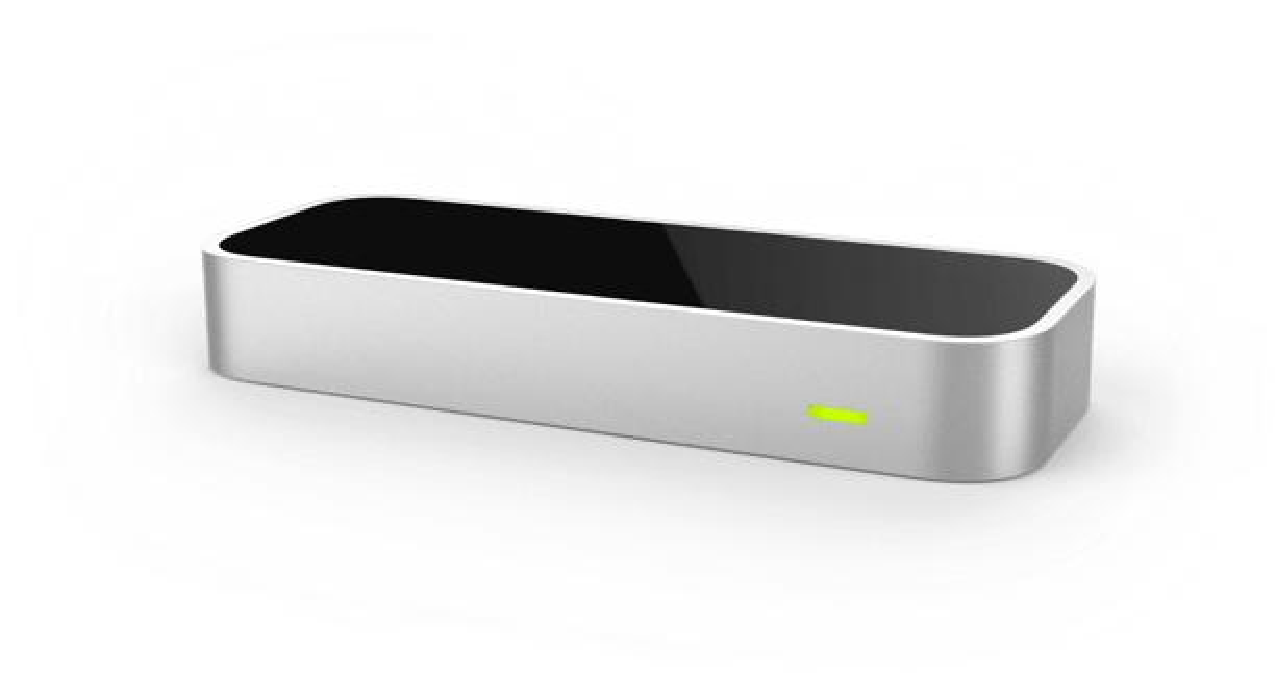
\includegraphics[width=\linewidth]{Figures/RadarExperiments/Sensors/lmc.pdf}
        \captionsetup{width=.99\linewidth}
        \caption{Sensor.}
        \label{fig:radar-experiments:lmc:product}
    \end{subfigure}
    \begin{subfigure}{.46\linewidth}
        \centering
        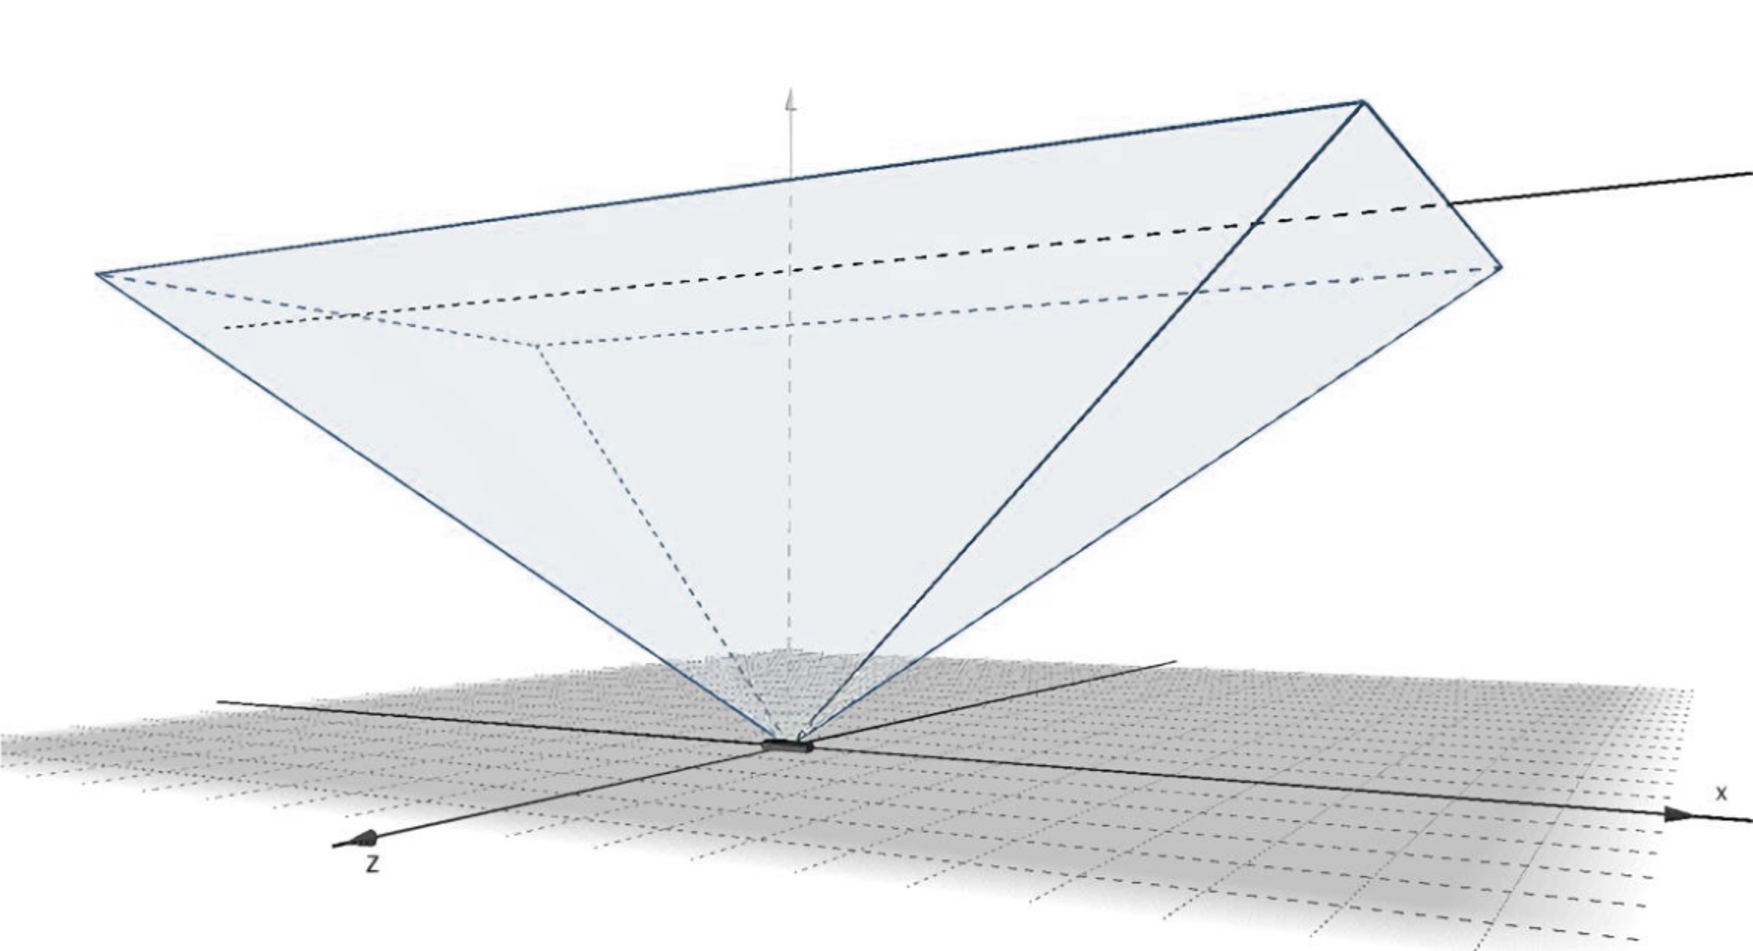
\includegraphics[width=\linewidth,trim={0.2cm 0.2cm 0.2cm 1.5cm},clip]{Figures/RadarExperiments/Sensors/lmc-fov.pdf}
        \captionsetup{width=.99\linewidth}
        \caption{Field of view.}
        \label{fig:radar-experiments:lmc:fov}
    \end{subfigure}
    \caption{The Leap Motion Controller.}
    \label{fig:radar-experiments:lmc}
\end{figure}

\subsubsection{LMC}
The LMC (\fig~\ref{fig:radar-experiments:lmc}) is a small, relatively inexpensive, and popular vision-based sensor for gesture recognition. It was described in detail in Section~\ref{sec:state_of_the_art:lmc} when we looked at the state of LMC-based gesture recognition in the literature. The LMC API provides hand skeletons that can be given as input to gesture recognition algorithms.

\subsubsection{Walabot}
The Walabot Developer is a commercially available, ultra-wideband (UWB) radar sensor employing frequency-modulated continuous-wave (FMCW) technology. It operates in the 6.3-8 GHz range in its EU/CE version and features an array of 18 bowtie radar antennas, including four used as transmitters and 15 as receivers (\fig~\ref{fig:radar-experiments:walabot}). The advantage of using an antenna array, as opposed to a monostatic or bistatic radar configuration, is its capability to furnish not only distance information but also direction information.
The compact form factor of the Walabot (72$\times$140 mm board) and its USB connectivity make it suitable for use in (semi-)mobile and stationary contexts of use. 
The Walabot Developer SDK enables the retrieval of raw time-domain radar data for use in custom applications. Three profiles are provided for distant scanning, defining the frequency range, the set of antenna pairs (right part of \fig~\ref{fig:radar-experiments:walabot}), the number of fast-time samples per frame, and the frame rate, as follows:
\begin{figure*}[!b]
    \vspace{-4pt}
    \centering
    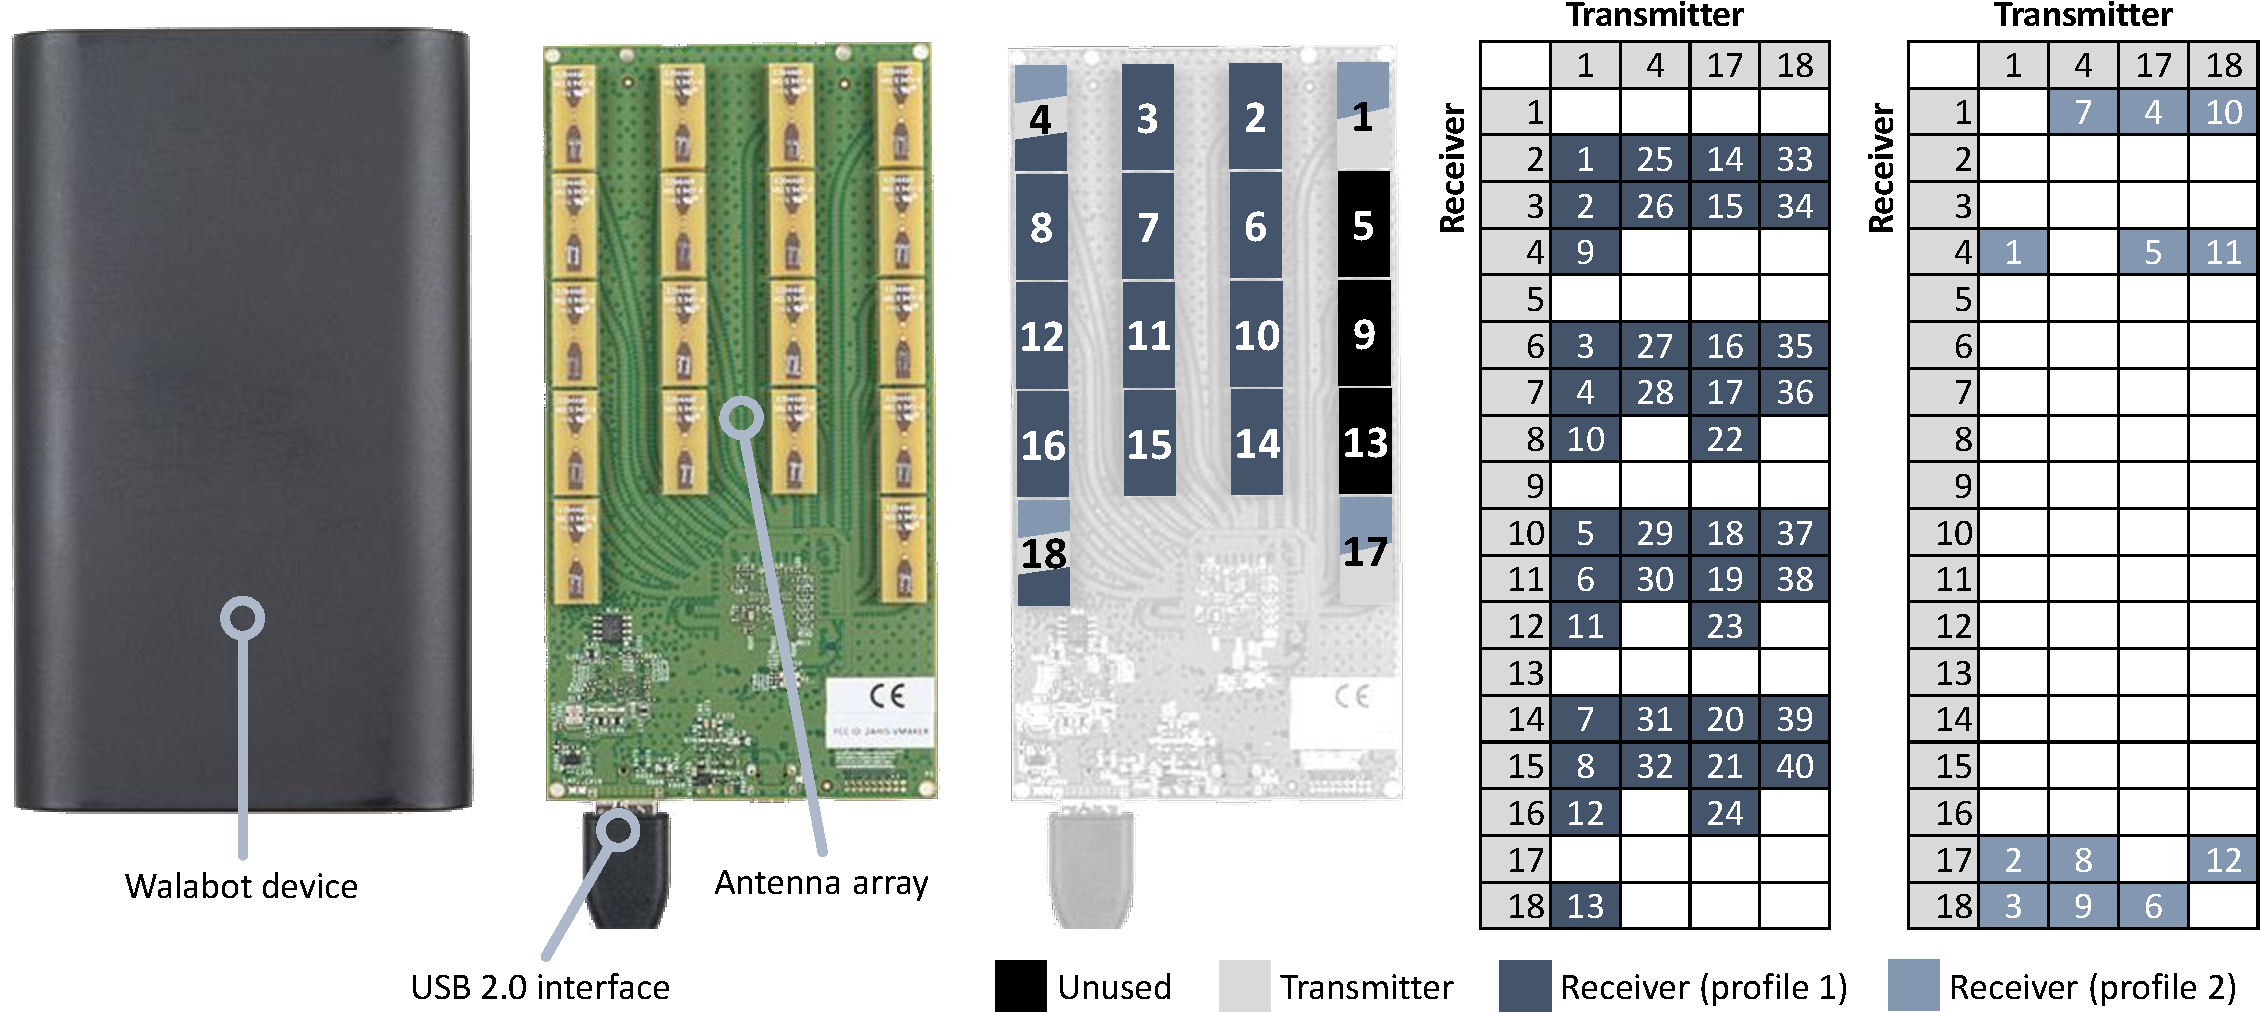
\includegraphics[width=\linewidth]{Figures/RadarExperiments/Sensors/walabot.pdf}
    \vspace{-16pt}
    \caption{Walabot enclosure and PCB, antennas IDs, and antenna pairs IDs (profiles 1 and 2).}
    \label{fig:radar-experiments:walabot}
\end{figure*}
\begin{itemize}
    \item Profile 1 (\custominlinecode{PROF_SENSOR}): 6.3-8 GHz range, 40 antenna pairs, 8192 fast-time samples/frame, \textasciitilde 20 fps.
    \item Profile 2 (\custominlinecode{PROF_SENSOR_NARROW}): 6.3-8 GHz range, 12 antenna pairs, 4096 fast-time samples/frame, \textasciitilde 41 fps.
    \item Profile 3 (\custominlinecode{PROF_WIDE_BAND}): 3.3-10 GHz range, 40 antenna pairs, 8192 fast time samples/frame, \textasciitilde 15 fps. This profile is only available with the US/FCC version of the Walabot.
\end{itemize}
The Walabot has been used in various application domains, including material identification~\cite{Agresti:2019}, activity recognition~\cite{Avrahami:2018, Zhu:2018}, and gesture recognition~\cite{Zhang:2021}.



\subsubsection{Custom Radar}
The ``horn'' (\fig~\ref{fig:radar-experiments:horn}) is a custom radar equipped with an antenna system consisting of a linearly polarized, double-ridged broadband horn antenna (BBHA 9120 A, Schwarzbeck Mess-Elektronik, Germany). The antenna dimensions are 22 cm (8.66 in.) long and 14$\times$24 cm$^2$ (5.51$\times$9.45 in.$^2$) aperture area. The antenna's nominal frequency range is 0.8 to 5 GHz, and its isotropic gain ranges from 6 to 18 dBi. The high directivity of the antenna (45\textdegree 3 dB beamwidth in the E-plane and 30\textdegree in the H-plane at 1 GHz) makes it suitable for gesture recognition.
This radar system provides very high range resolution, but low angular resolution as it features only one antenna.

\begin{figure}[!h]
    \centering
    \includegraphics[width=.35\linewidth,trim={2pt 2pt 2pt 2pt},clip]{Figures/RadarExperiments/Sensors/horn-antenna.pdf}
    % \vspace{-12pt}
    \caption{Custom radar.}
    \label{fig:radar-experiments:horn}
    % \vspace{-14pt}
\end{figure}


%--------------------------------------------------------------------------------%
\subsection{Datasets} \label{sec:radar-experiments:data-collection:datasets}
Three datasets were designed to evaluate the radar data processing strategy in different conditions (\tab~\ref{tab:radar-experiments:datasets-summary}). Their gestures are compiled in \fig~\ref{fig:radar-experiments:gestures-a},~\ref{fig:radar-experiments:gestures-b}, and~\ref{fig:radar-experiments:gestures-c}. Each gesture is classified according to Aigner \etal's taxonomy~\cite{Aigner:2012} and our taxonomy, inspired by Vatavu's iFad gestures~\cite{Vatavu:2023b} (\fig~\ref{fig:radar-experiments:taxonomy}).

\begin{table}[!b]
    \footnotesize
    \centering
    \begin{tabular}{lrrrp{4.6cm}}
        \toprule
        \textbf{Name} & \textbf{Classes} & \textbf{Users} & \textbf{Samples} & \textbf{Sensor(s)} \\
        \midrule
        Sensors comparison & 16 & 1 & 320 & Walabot, Custom radar, LMC\\
        20-gestures & 20 & 6 & 1200 & Walabot \\
        Through-materials & 9 & 20 & 2700 & Walabot with wood, PVC, and glass \\
        \bottomrule
    \end{tabular}
    \caption{Summary of the datasets used in the three experiments.}
    \label{tab:radar-experiments:datasets-summary}
\end{table}

\begin{figure}[b]
    \centering
    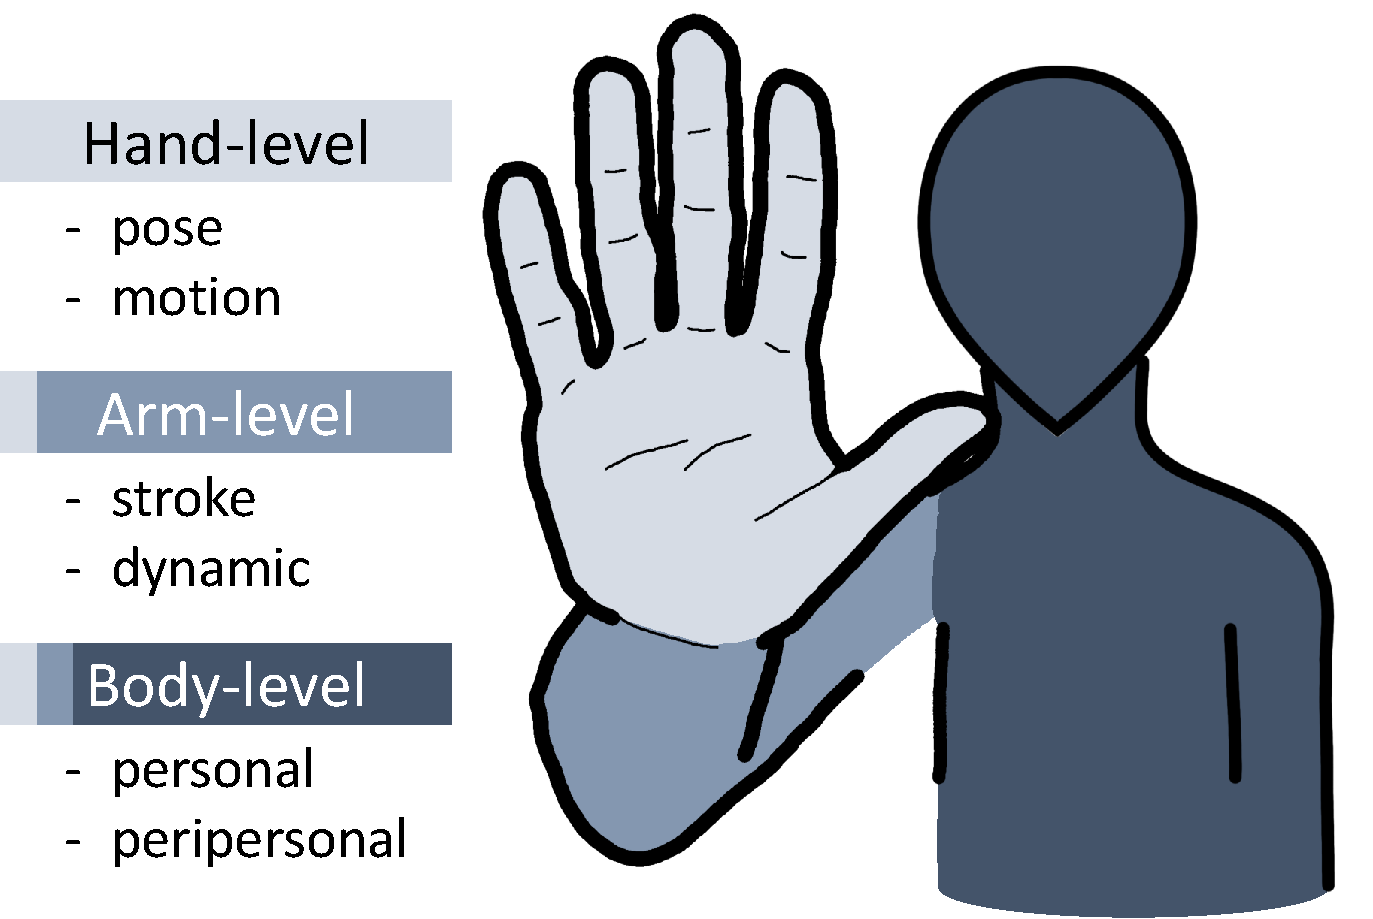
\includegraphics[width=.60\linewidth]{Figures/RadarExperiments/Datasets/20Gestures/gesture-taxonomy.pdf}
    \vspace{-2pt}
    \caption{Taxonomy inspired by Vatavu's iFAD gestures~\cite{Vatavu:2023b}.}
    \label{fig:radar-experiments:taxonomy}
    \vspace{-6pt}
\end{figure}

\begin{figure*}
    \centering
    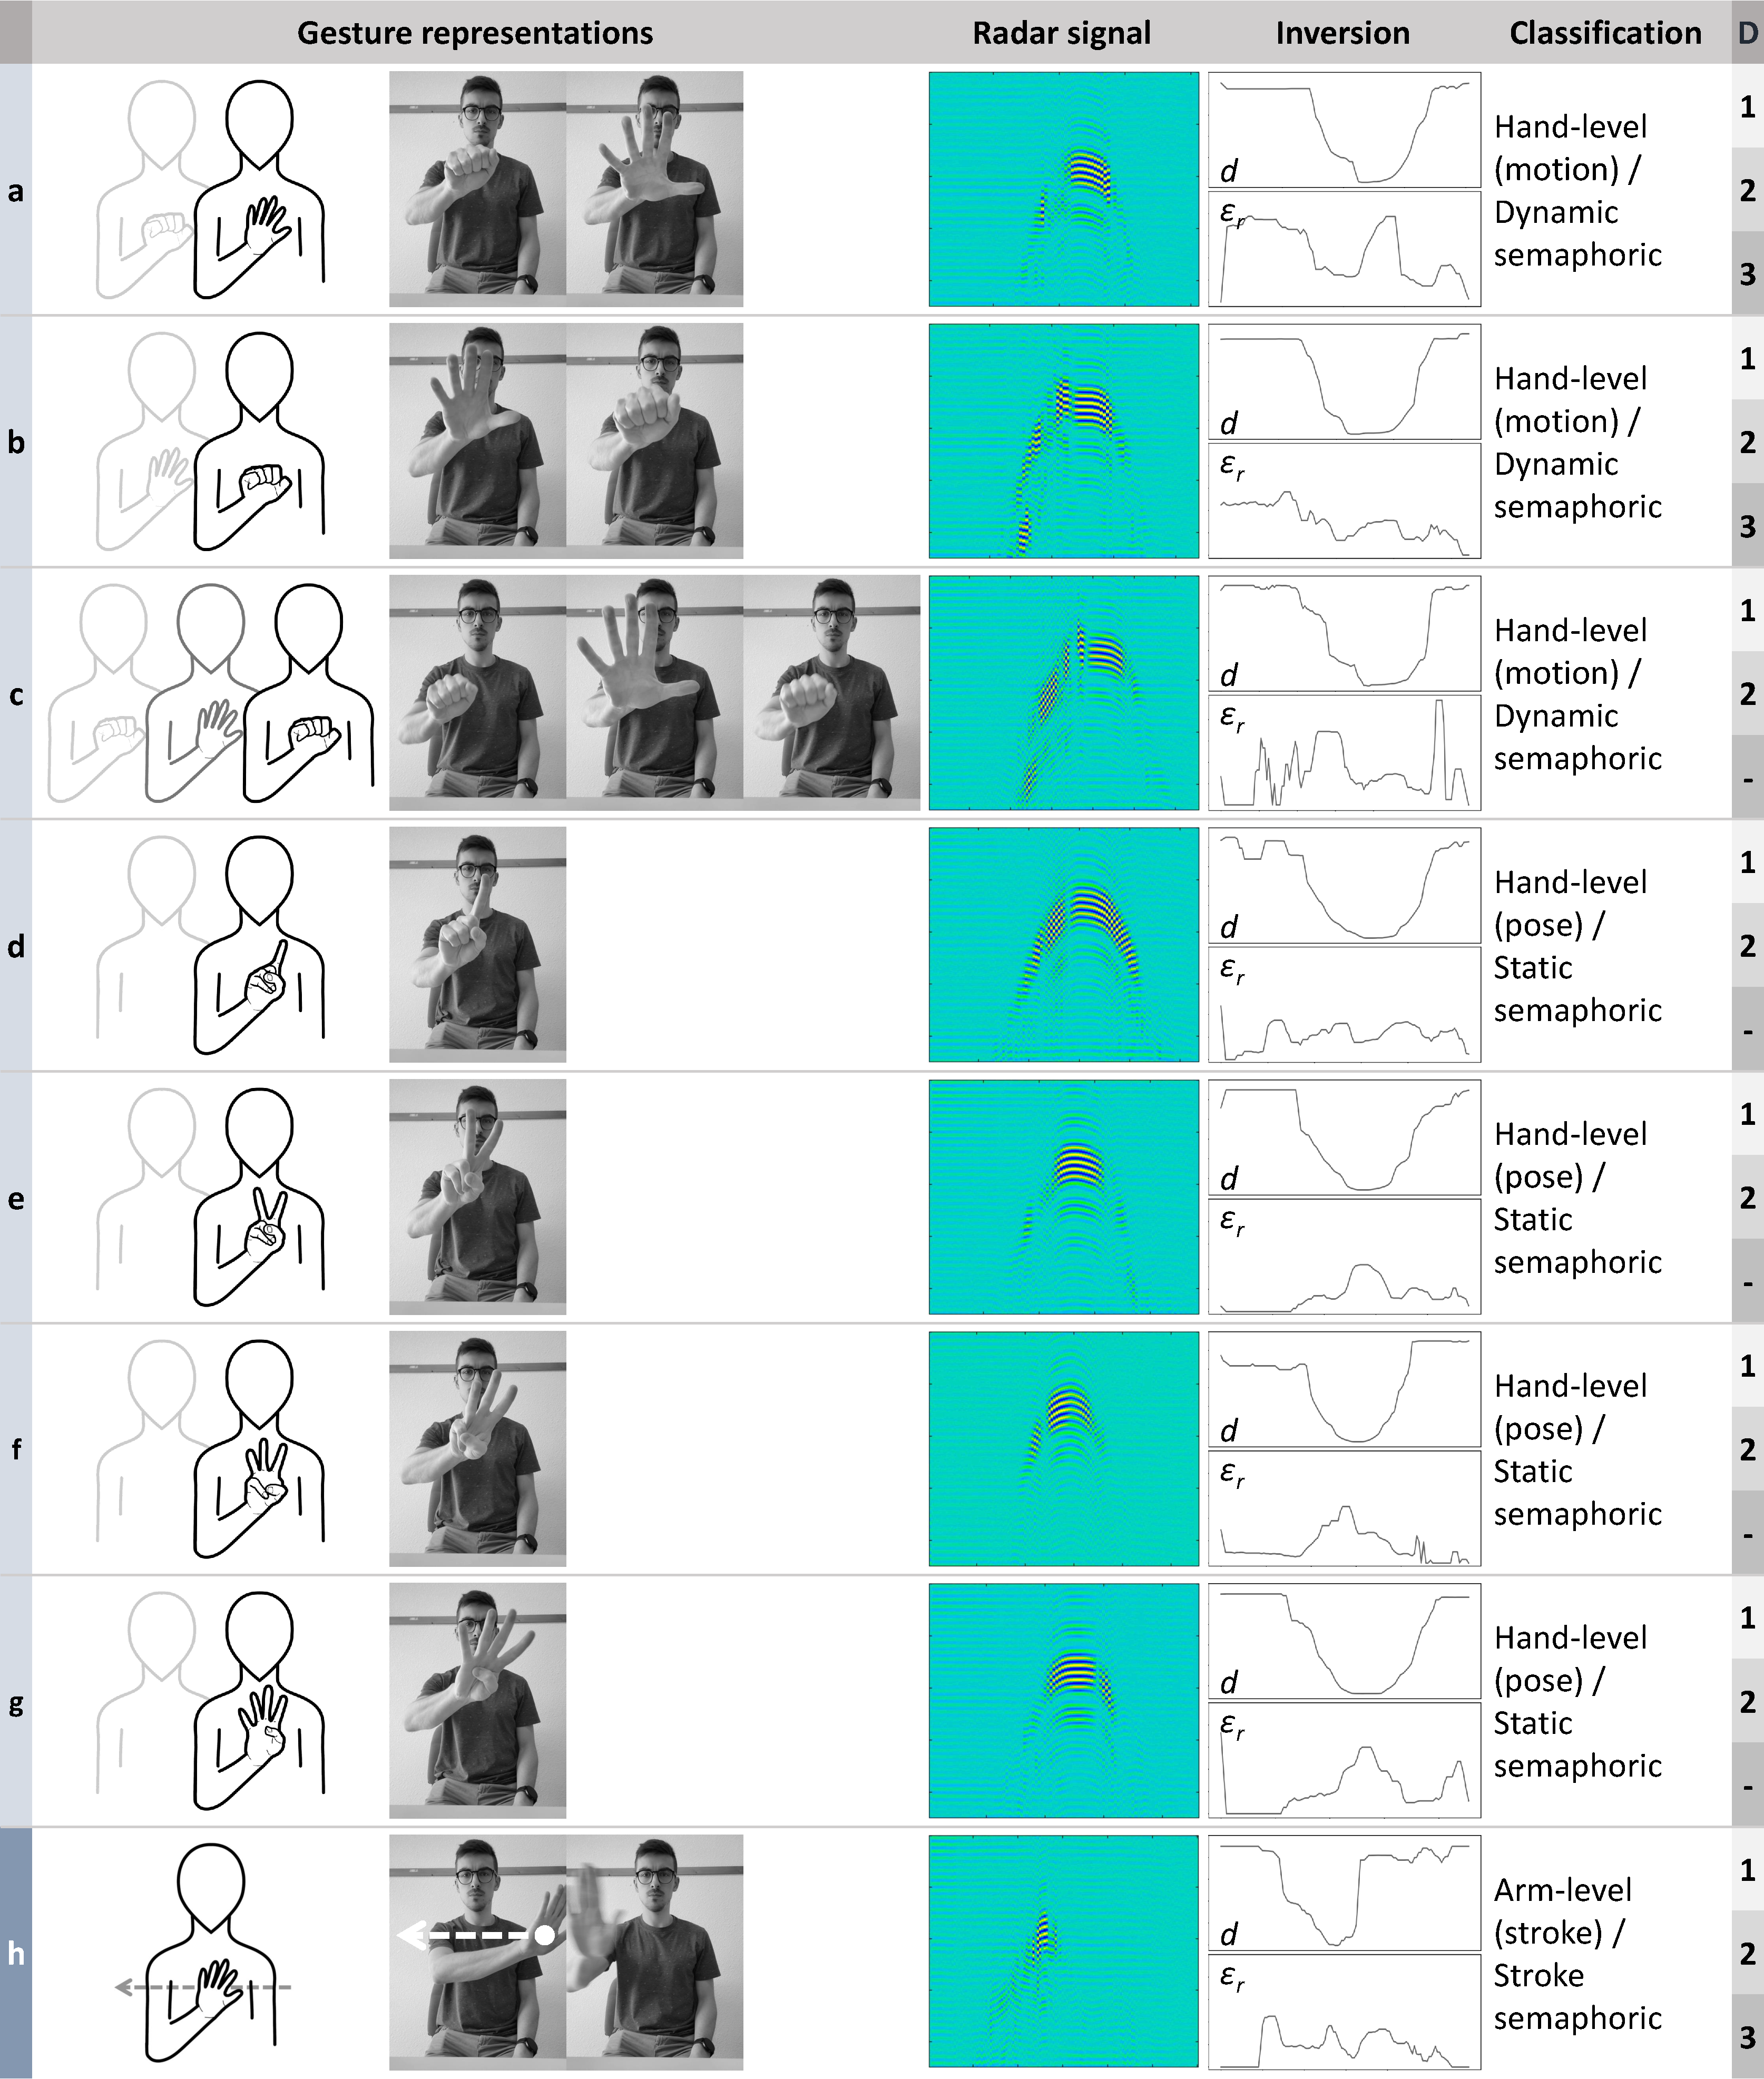
\includegraphics[width=\linewidth]{Figures/RadarExperiments/Datasets/gesture-table-new-1.pdf}
    % \vspace{-8pt}
    \caption{Consolidation of all gestures from the three radar datasets and their classification according to our gesture taxonomy (\fig~\ref{fig:radar-experiments:taxonomy}) and the taxonomy of Aigner \etal~\cite{Aigner:2012}.}
    \label{fig:radar-experiments:gestures-a}
    \vspace{-8pt}
\end{figure*}

\begin{figure*}
    \centering
    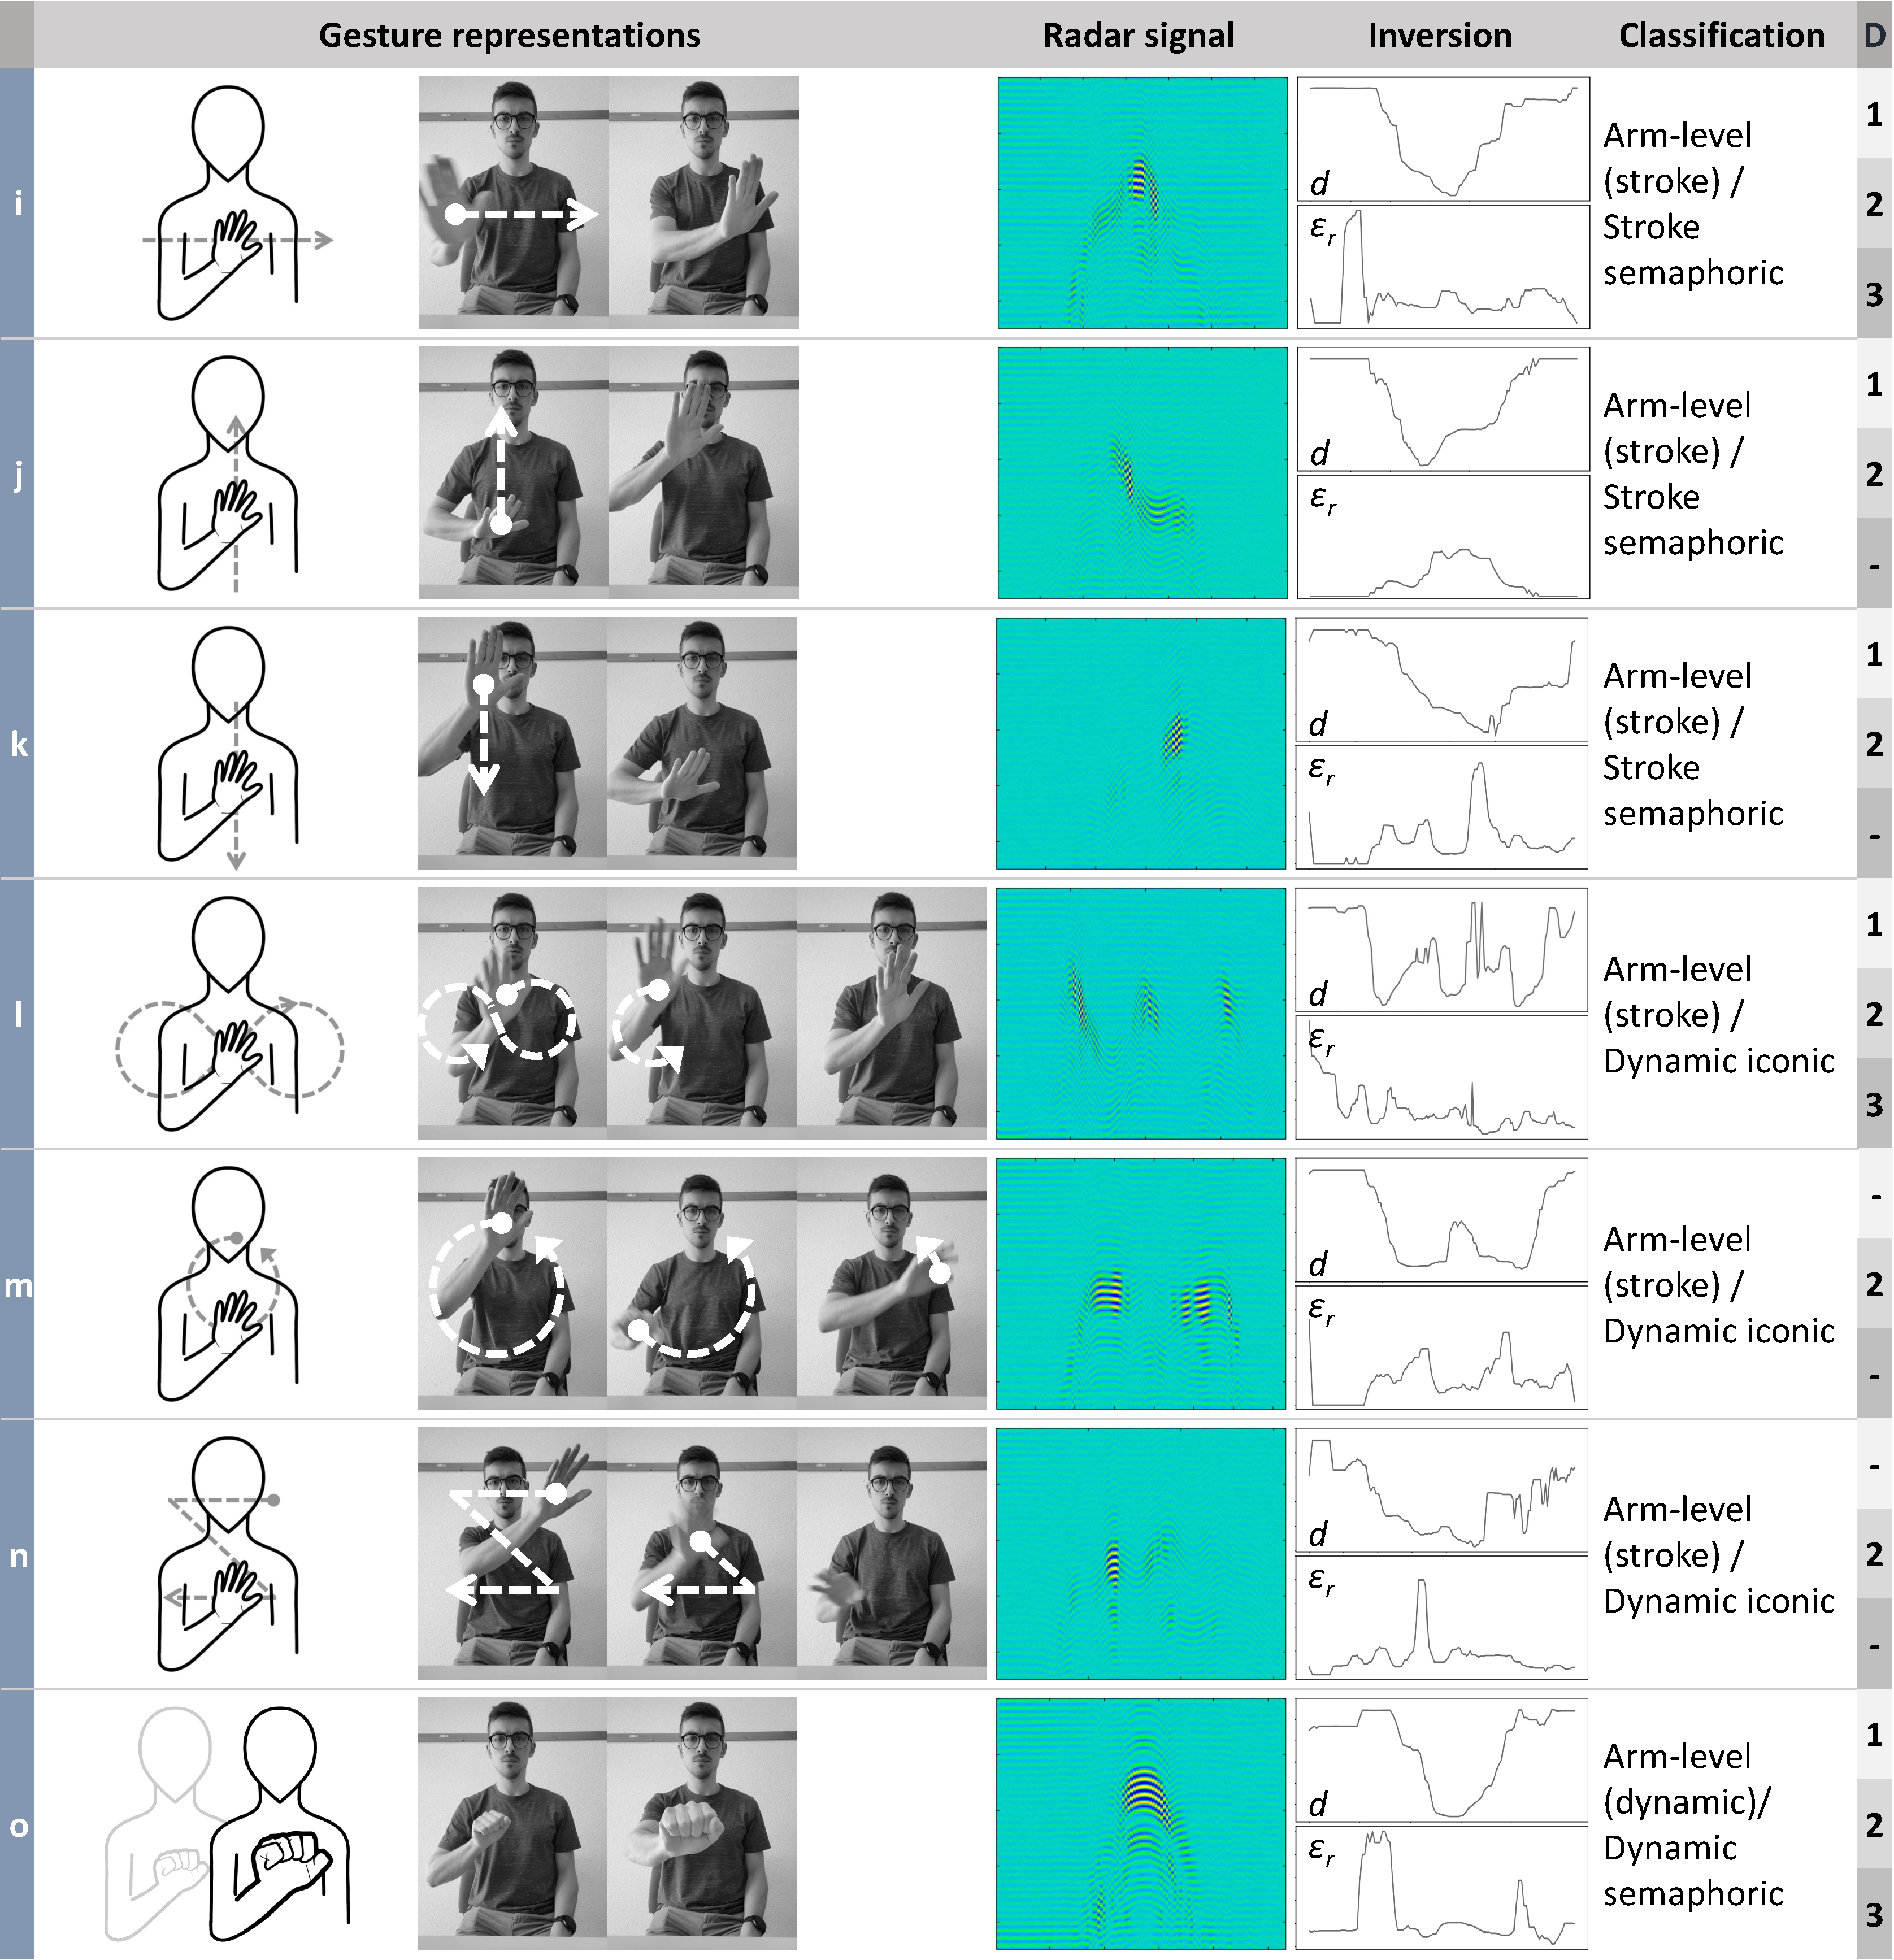
\includegraphics[width=\linewidth]{Figures/RadarExperiments/Datasets/gesture-table-new-2.pdf}
    % \vspace{-8pt}
    \caption{Consolidation of all gestures from the three radar datasets and their classification according to our gesture taxonomy (\fig~\ref{fig:radar-experiments:taxonomy}) and the taxonomy of Aigner \etal~\cite{Aigner:2012} (cont.).}
    \label{fig:radar-experiments:gestures-b}
    \vspace{-8pt}
\end{figure*}

\begin{figure*}
    \centering
    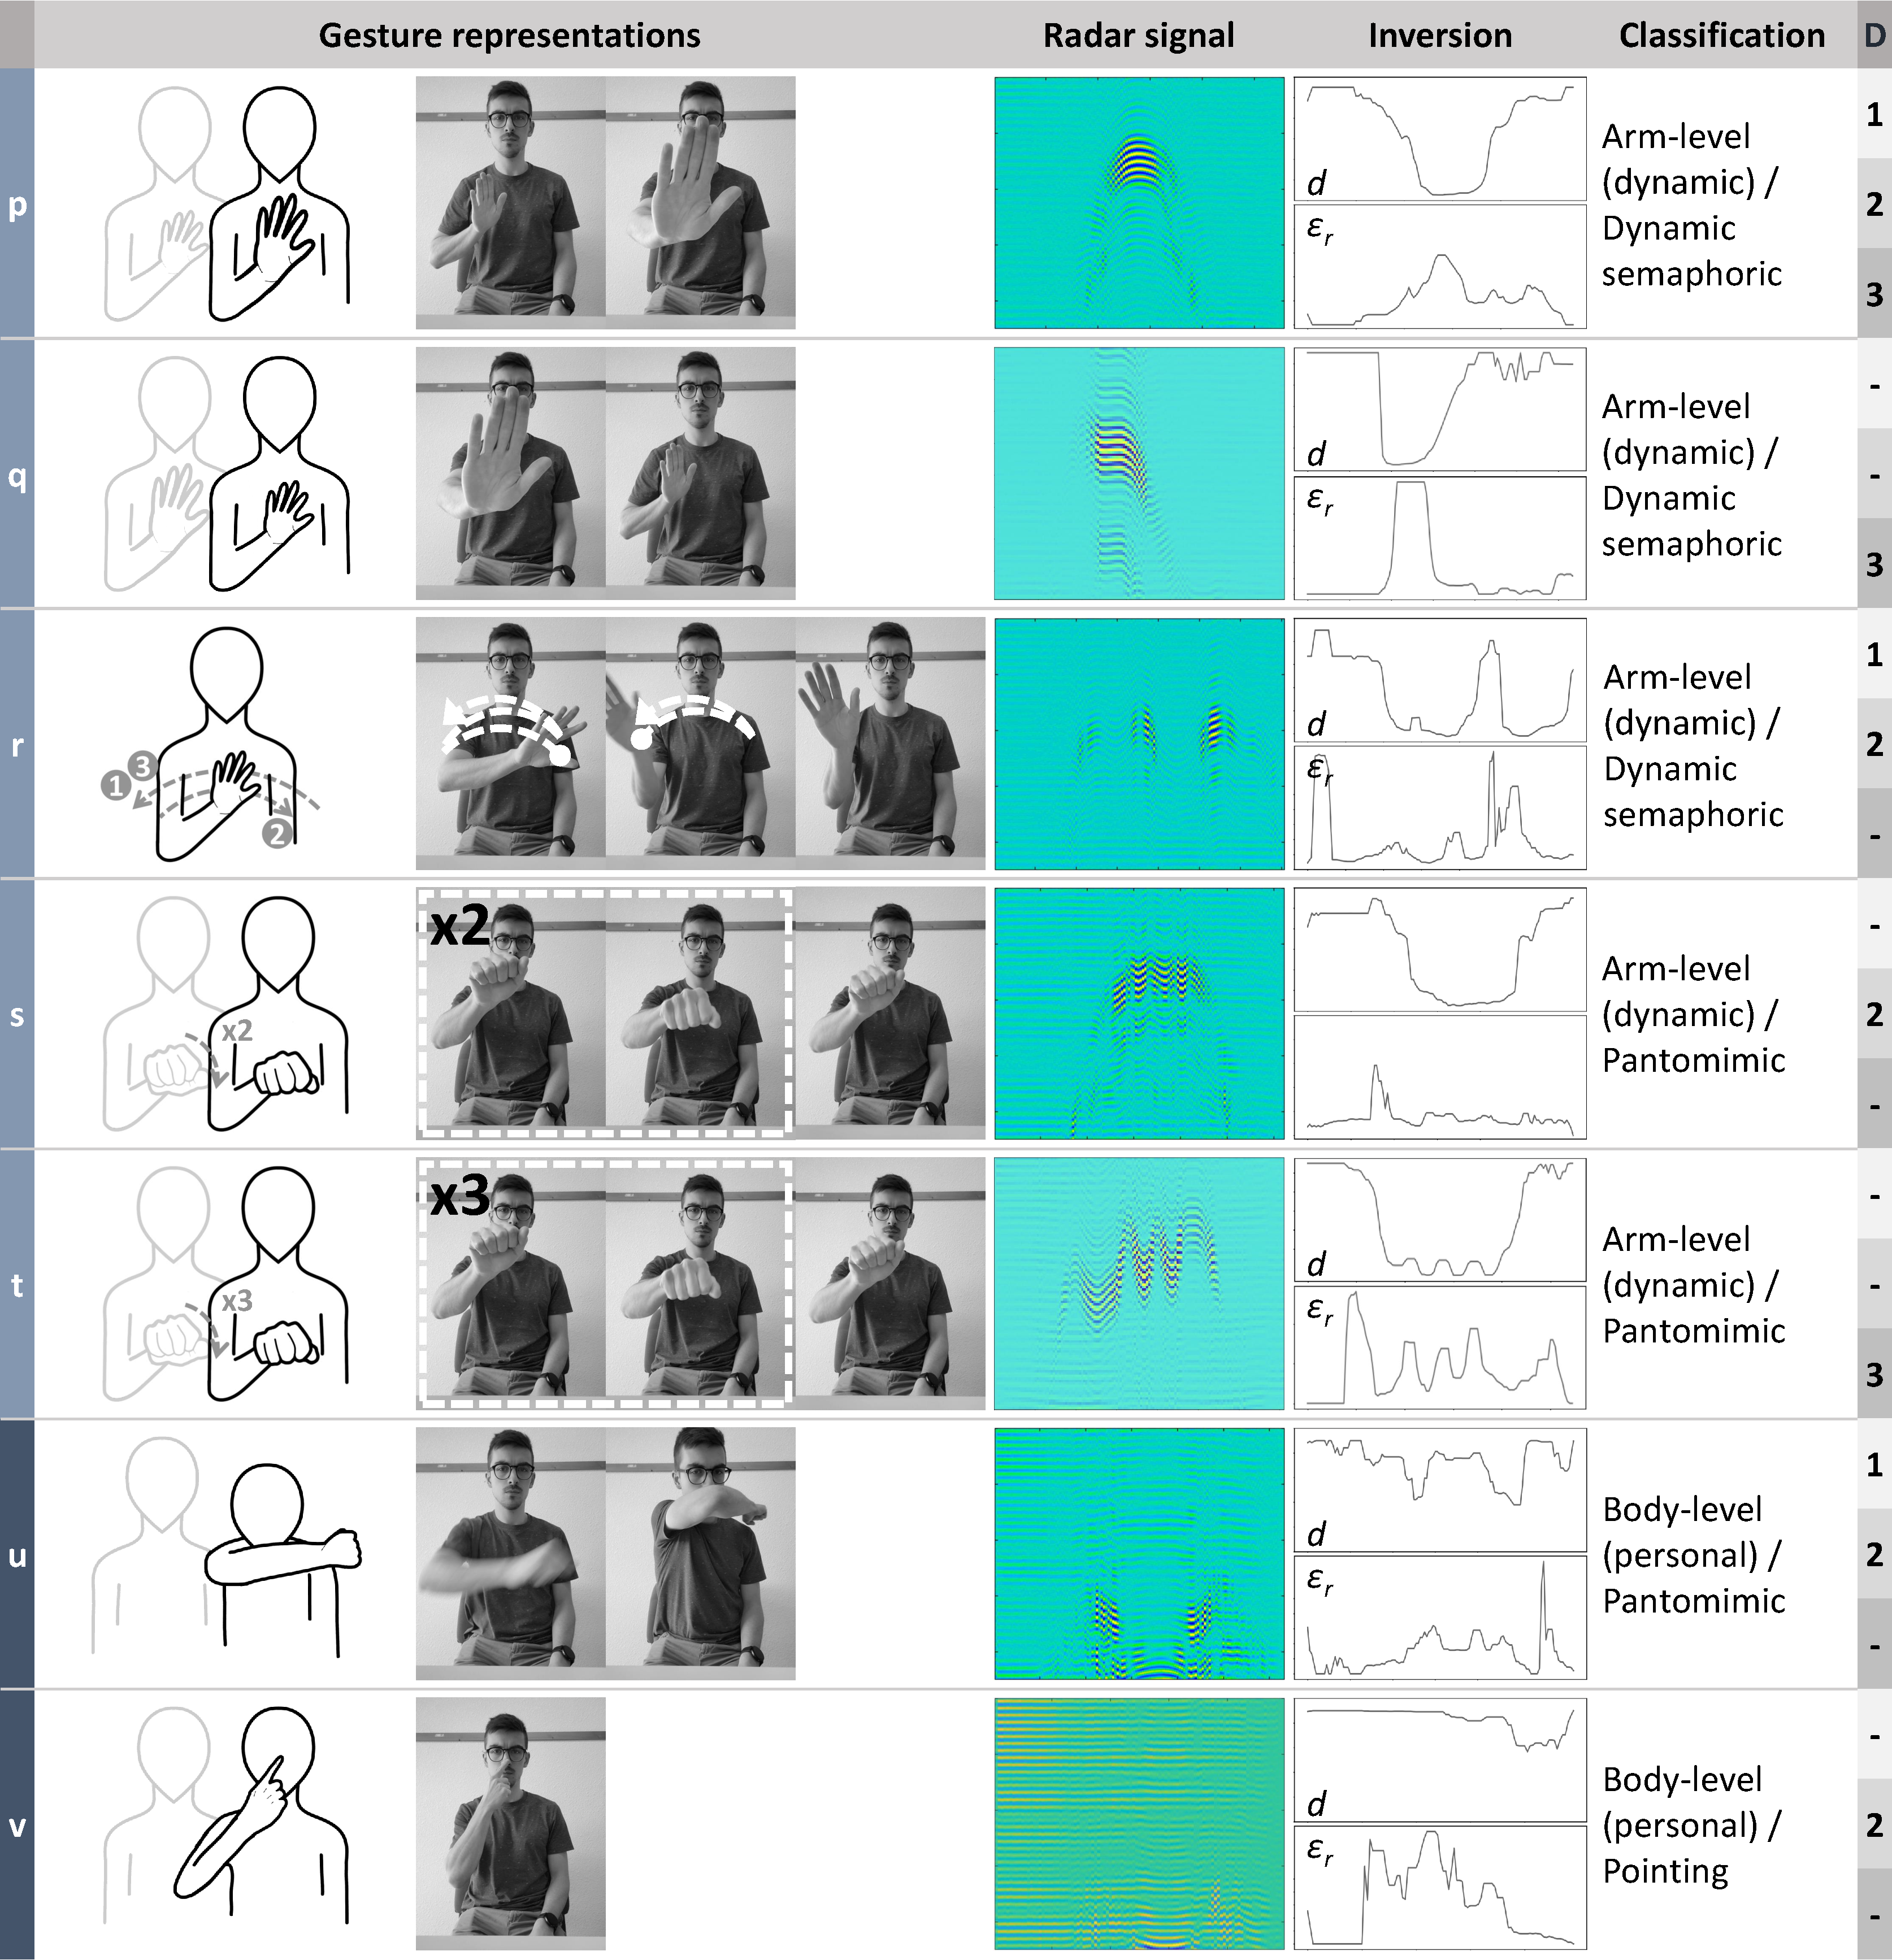
\includegraphics[width=\linewidth]{Figures/RadarExperiments/Datasets/gesture-table-new-3.pdf}
    % \vspace{-8pt}
    \caption{Consolidation of all gestures from the three radar datasets and their classification according to our gesture taxonomy (\fig~\ref{fig:radar-experiments:taxonomy}) and the taxonomy of Aigner \etal~\cite{Aigner:2012} (cont.).}
    \label{fig:radar-experiments:gestures-c}
    \vspace{-8pt}
\end{figure*}

\subsubsection{Sensors Comparison} \label{sec:radar-experiments:data-collection:datasets:sensors}
A set of 16 gestures was designed by consolidating results obtained in \cite{Palipana:2021,Hayashi:2021,Lien:2016} and in a GES: (a) open hand, (b) close hand, (c) open then close hand, (d) extend one finger, (e) extend two fingers, (f) extend three fingers, (g) extend four fingers, (h) swipe right, (i) swipe left, (j) swipe up, (k) swipe down, (l) draw infinity, (o) push fist, (p) push palm, (r) hello, and (u) barrier gesture.

Each gesture was performed by one right-handed participant (male, 55 years old, with no prior experience with radar gestures) and recorded with three different devices, namely an LMC, a Walabot, and a custom radar (horn). Because the overlap between the frequency ranges of the two radars risked producing interference, we decided to record the dataset in two sessions: (1) simultaneously with the LMC and the Walabot, and (2) simultaneously with the LMC and the custom radar. 
In both sessions, the radar was positioned at a distance of about 70 cm in front of the subject, enough to ensure that the far-field hypothesis of the antenna model was valid at all times (see Section~\ref{sec:radar-challenges:mathematical-theory:radar-model}). It was separated from the table by an empty cardboard box, a material relatively transparent to RF waves, with a height of 26 cm. The LMC was placed on the desk, under the participant's hand. The setup for both sessions is shown in \fig~\ref{fig:radar-experiments:setup-sensors-comparison:walabot-lmc} and~\ref{fig:radar-experiments:setup-sensors-comparison:horn-lmc}.

The participant produced five repetitions of each gesture type in a controlled environment, resulting in a total of 16 (gestures) $\times$ 1 (participant) $\times$ 5 (repetitions) $=$ 80 samples per sensor. 
The recording procedure was as follows (\fig~\ref{fig:radar-experiments:gestures-stages}): show the gesture to the participant, then, for each sample (1) the participant starts with their hands on their laps, (2) the recording is started, (3) the participant produces the gesture, (4) the participant places their hands back on their laps, (5) the recording is stopped and the data is saved to a text file. This sequence of actions was repeated for each repetition of each gesture and each sensor. LMC data was recorded simultaneously with the Walabot/custom radar data at around 100 frames per second using custom software.
The Walabot was configured to record with 12 antenna pairs at around 40 frames per second (\custominlinecode{PROF_SENSOR_NARROW} profile). It produced time-domain data that was truncated to keep only the first 1024 fast-time samples out of 4096 to maximize the recording framerate.
The custom radar produced frequency-domain data at about ten frames per second.

\begin{figure}[t]
    \centering
    \begin{subfigure}{.53\linewidth}
        \centering
        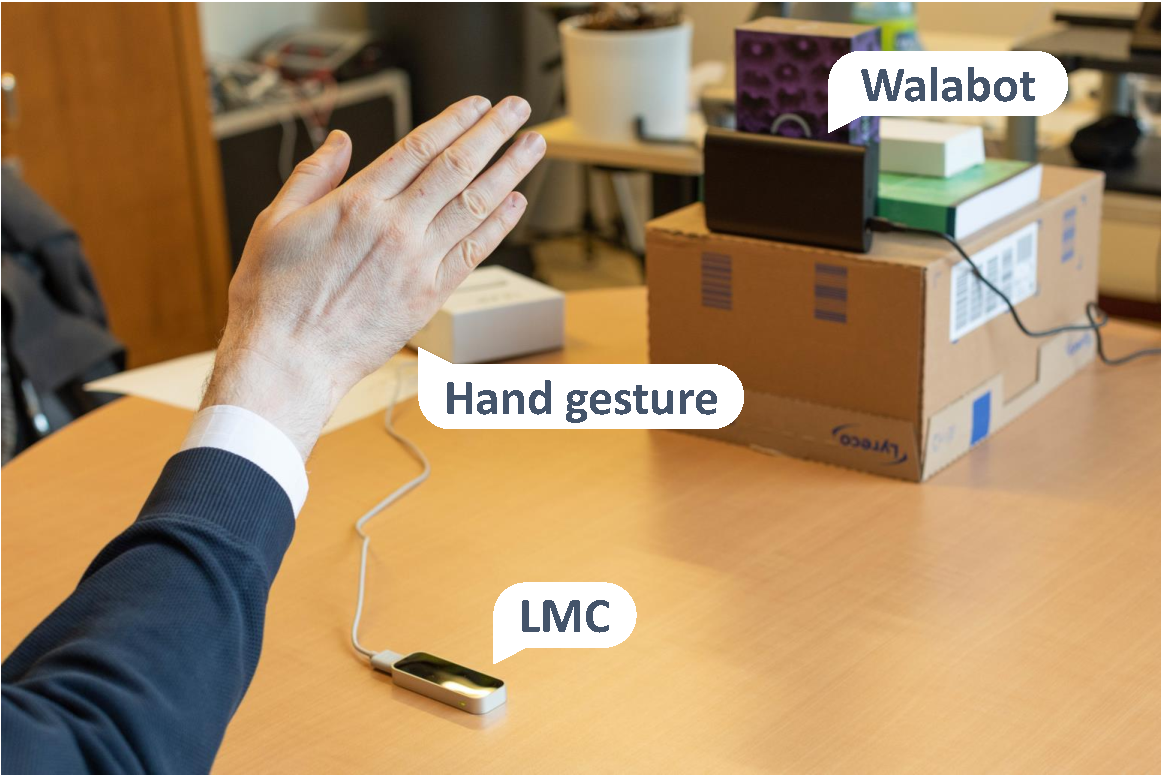
\includegraphics[width=\linewidth]{Figures/RadarExperiments/Datasets/SensorsComparison/setup-walabot-lmc.pdf}
        \captionsetup{width=.99\linewidth}
        \caption{Walabot and LMC.}
        \label{fig:radar-experiments:setup-sensors-comparison:walabot-lmc}
    \end{subfigure}
    \begin{subfigure}{.46\linewidth}
        \centering
        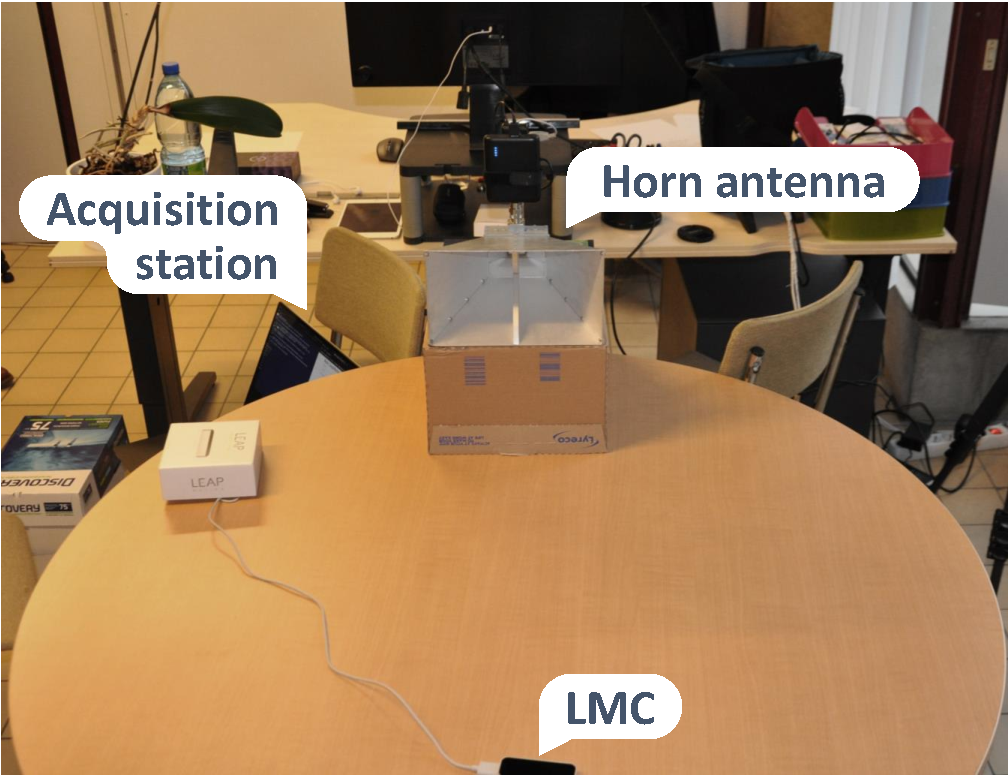
\includegraphics[width=\linewidth]{Figures/RadarExperiments/Datasets/SensorsComparison/setup-horn-lmc.pdf}
        \captionsetup{width=.99\linewidth}
        \caption{Custom radar and LMC.}
        \label{fig:radar-experiments:setup-sensors-comparison:horn-lmc}
    \end{subfigure}
    \vspace{-16pt}
    \caption{Setup used for acquiring the ``sensors comparison'' dataset.}
    \label{fig:radar-experiments:setup-sensors-comparison}
\end{figure}

\begin{figure*}[bt]
    \centering
    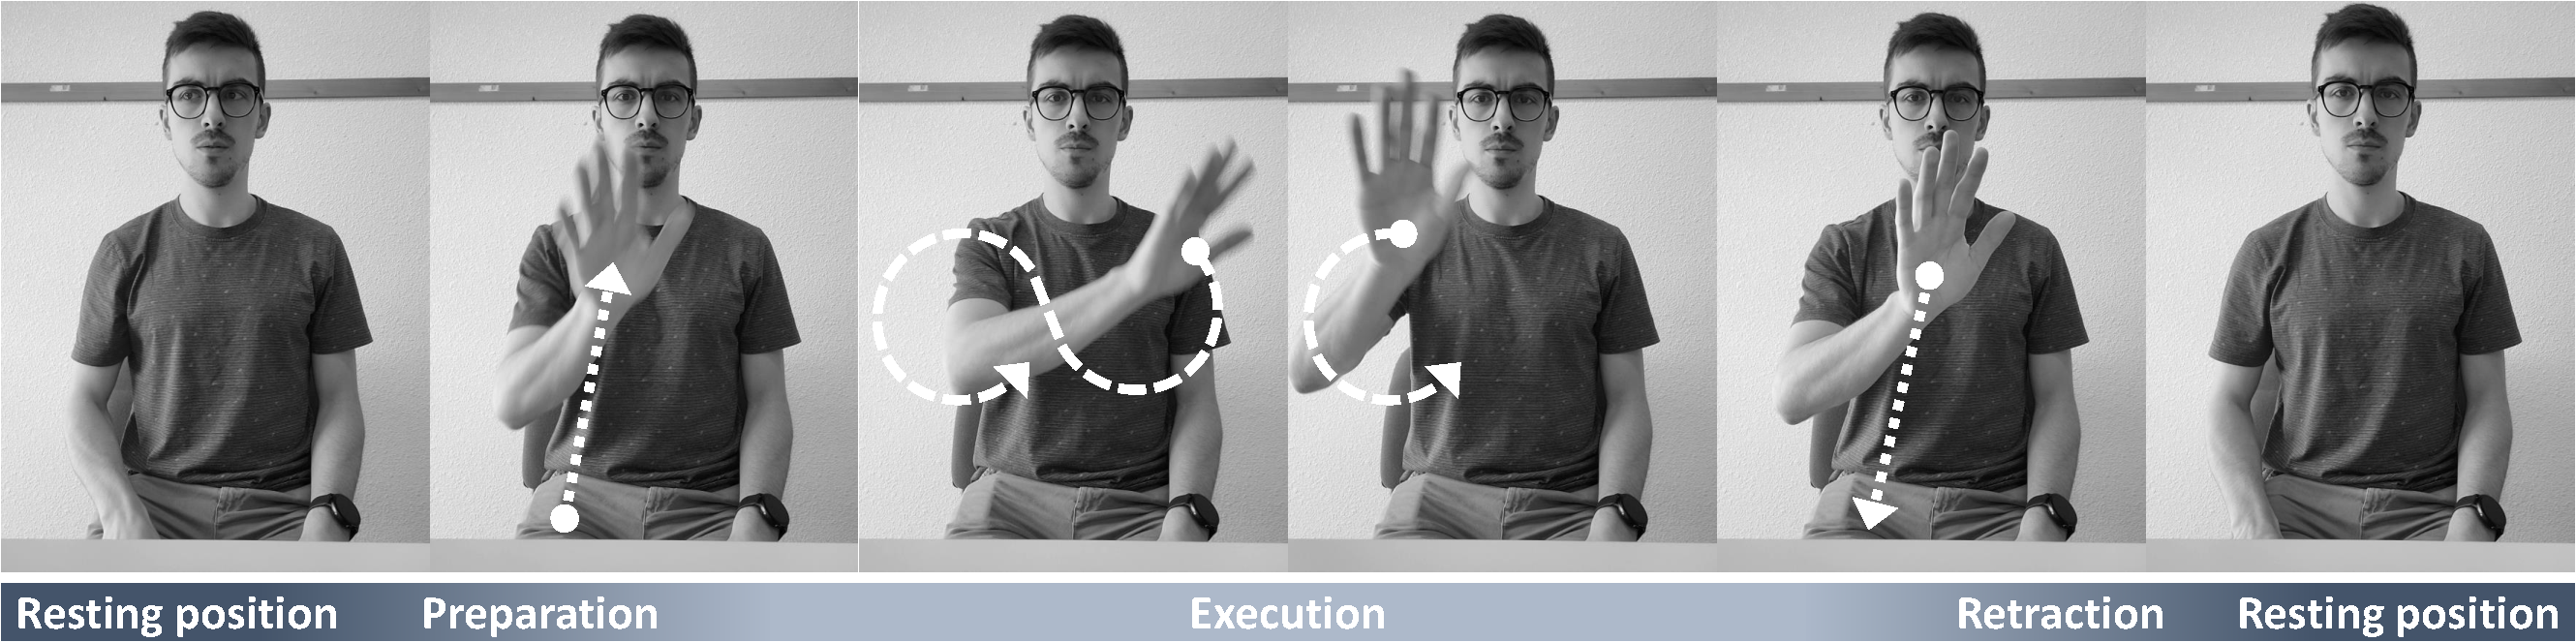
\includegraphics[width=\linewidth]{Figures/RadarExperiments/Datasets/20Gestures/gesture_stages.pdf}
    % \vspace{-8pt}
    \caption{The five phases of a gesture, based on \cite{Kendon:1980}.}
    \label{fig:radar-experiments:gestures-stages}
\end{figure*}


\subsubsection{20-gestures Dataset} \label{sec:radar-experiments:data-collection:datasets:20-gestures}
The second dataset is an extension of the previous dataset with four additional gestures, totaling 20 gestures: (a) open hand, (b) close hand, (c) open then close hand, (d) extend one finger, (e) extend two fingers, (f) extend three fingers, (g) extend four fingers, (h) swipe right, (i) swipe left, (j) swipe up, (k) swipe down, (l) draw infinity, (m) draw circle, (n) draw Z, (o) push fist, (p) push palm, (r) hello, (s) knock twice, (u) barrier gesture, and (v) touch nose.

\begin{figure}[hbt]
    \centering
    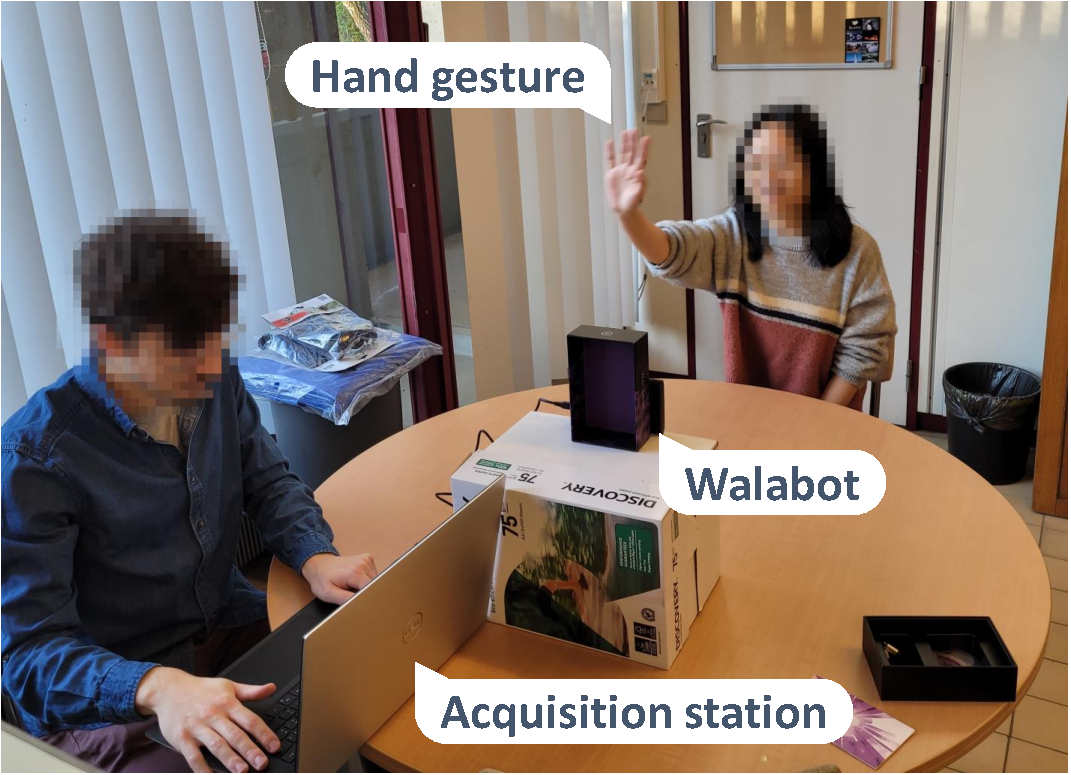
\includegraphics[width=.6\linewidth]{Figures/RadarExperiments/Datasets/20Gestures/setup-walabot-only.pdf}
    \caption{Setup used for acquiring the ``20-gestures'' dataset.}
    \label{fig:radar-experiments:setup:walabot-only}
\end{figure}

Each gesture was performed ten times by six participants in a controlled environment and recorded with a Walabot device, resulting in a total of 20 (gestures) $\times$ 6 (participants) $\times$ 10 (repetitions) ${=}$ 1200 samples. 
%
The setup (\fig~\ref{fig:radar-experiments:setup:walabot-only}) and recording procedure were similar to the first dataset, with the difference being that we only used a Walabot for recording.
On average, a recording session (\ie record ten samples for each of the 20 gestures) took around 30 minutes. 

\subsubsection{Through-materials} \label{sec:radar-experiments:data-collection:datasets:through-materials}
The third dataset consists of nine frequent gestures selected based on our experience with the previous datasets: (a) open hand, (b) close hand, (h) swipe right, (i) swipe left, (l) draw infinity, (o) push fist, (p) push palm, (q) pull palm, and (t) knock three times. 

All gestures were recorded with three Walabot devices, each attached to the back of a 1 m $\times$ 1 m plate of a different material (see Fig~\ref{fig:radar-experiments:setup-walabot-materials}): (1) wood (1.7 cm thick), (2) PVC (0.9 cm thick), and (3) glass (0.5 cm thick).
While not as extensive as in the work of Pucihar \etal~\cite{Pucihar:2022}, this set of materials covers a wide variety of real-world contexts of use and many potential scenarios in which hand gesture recognition could be deployed. For instance, all three materials are used in furniture and as construction materials while some toys are made of wood and PVC. 
Participants performed gestures while standing up in front of the material.
Each material was placed on an easel with its height adjusted so that the participant's right hand faced the Walabot with their arm extended. The distance between the participant's hand and the material was 20 cm. The Walabot configuration was the same as in the other two datasets.

\begin{figure}[t]
    \centering
    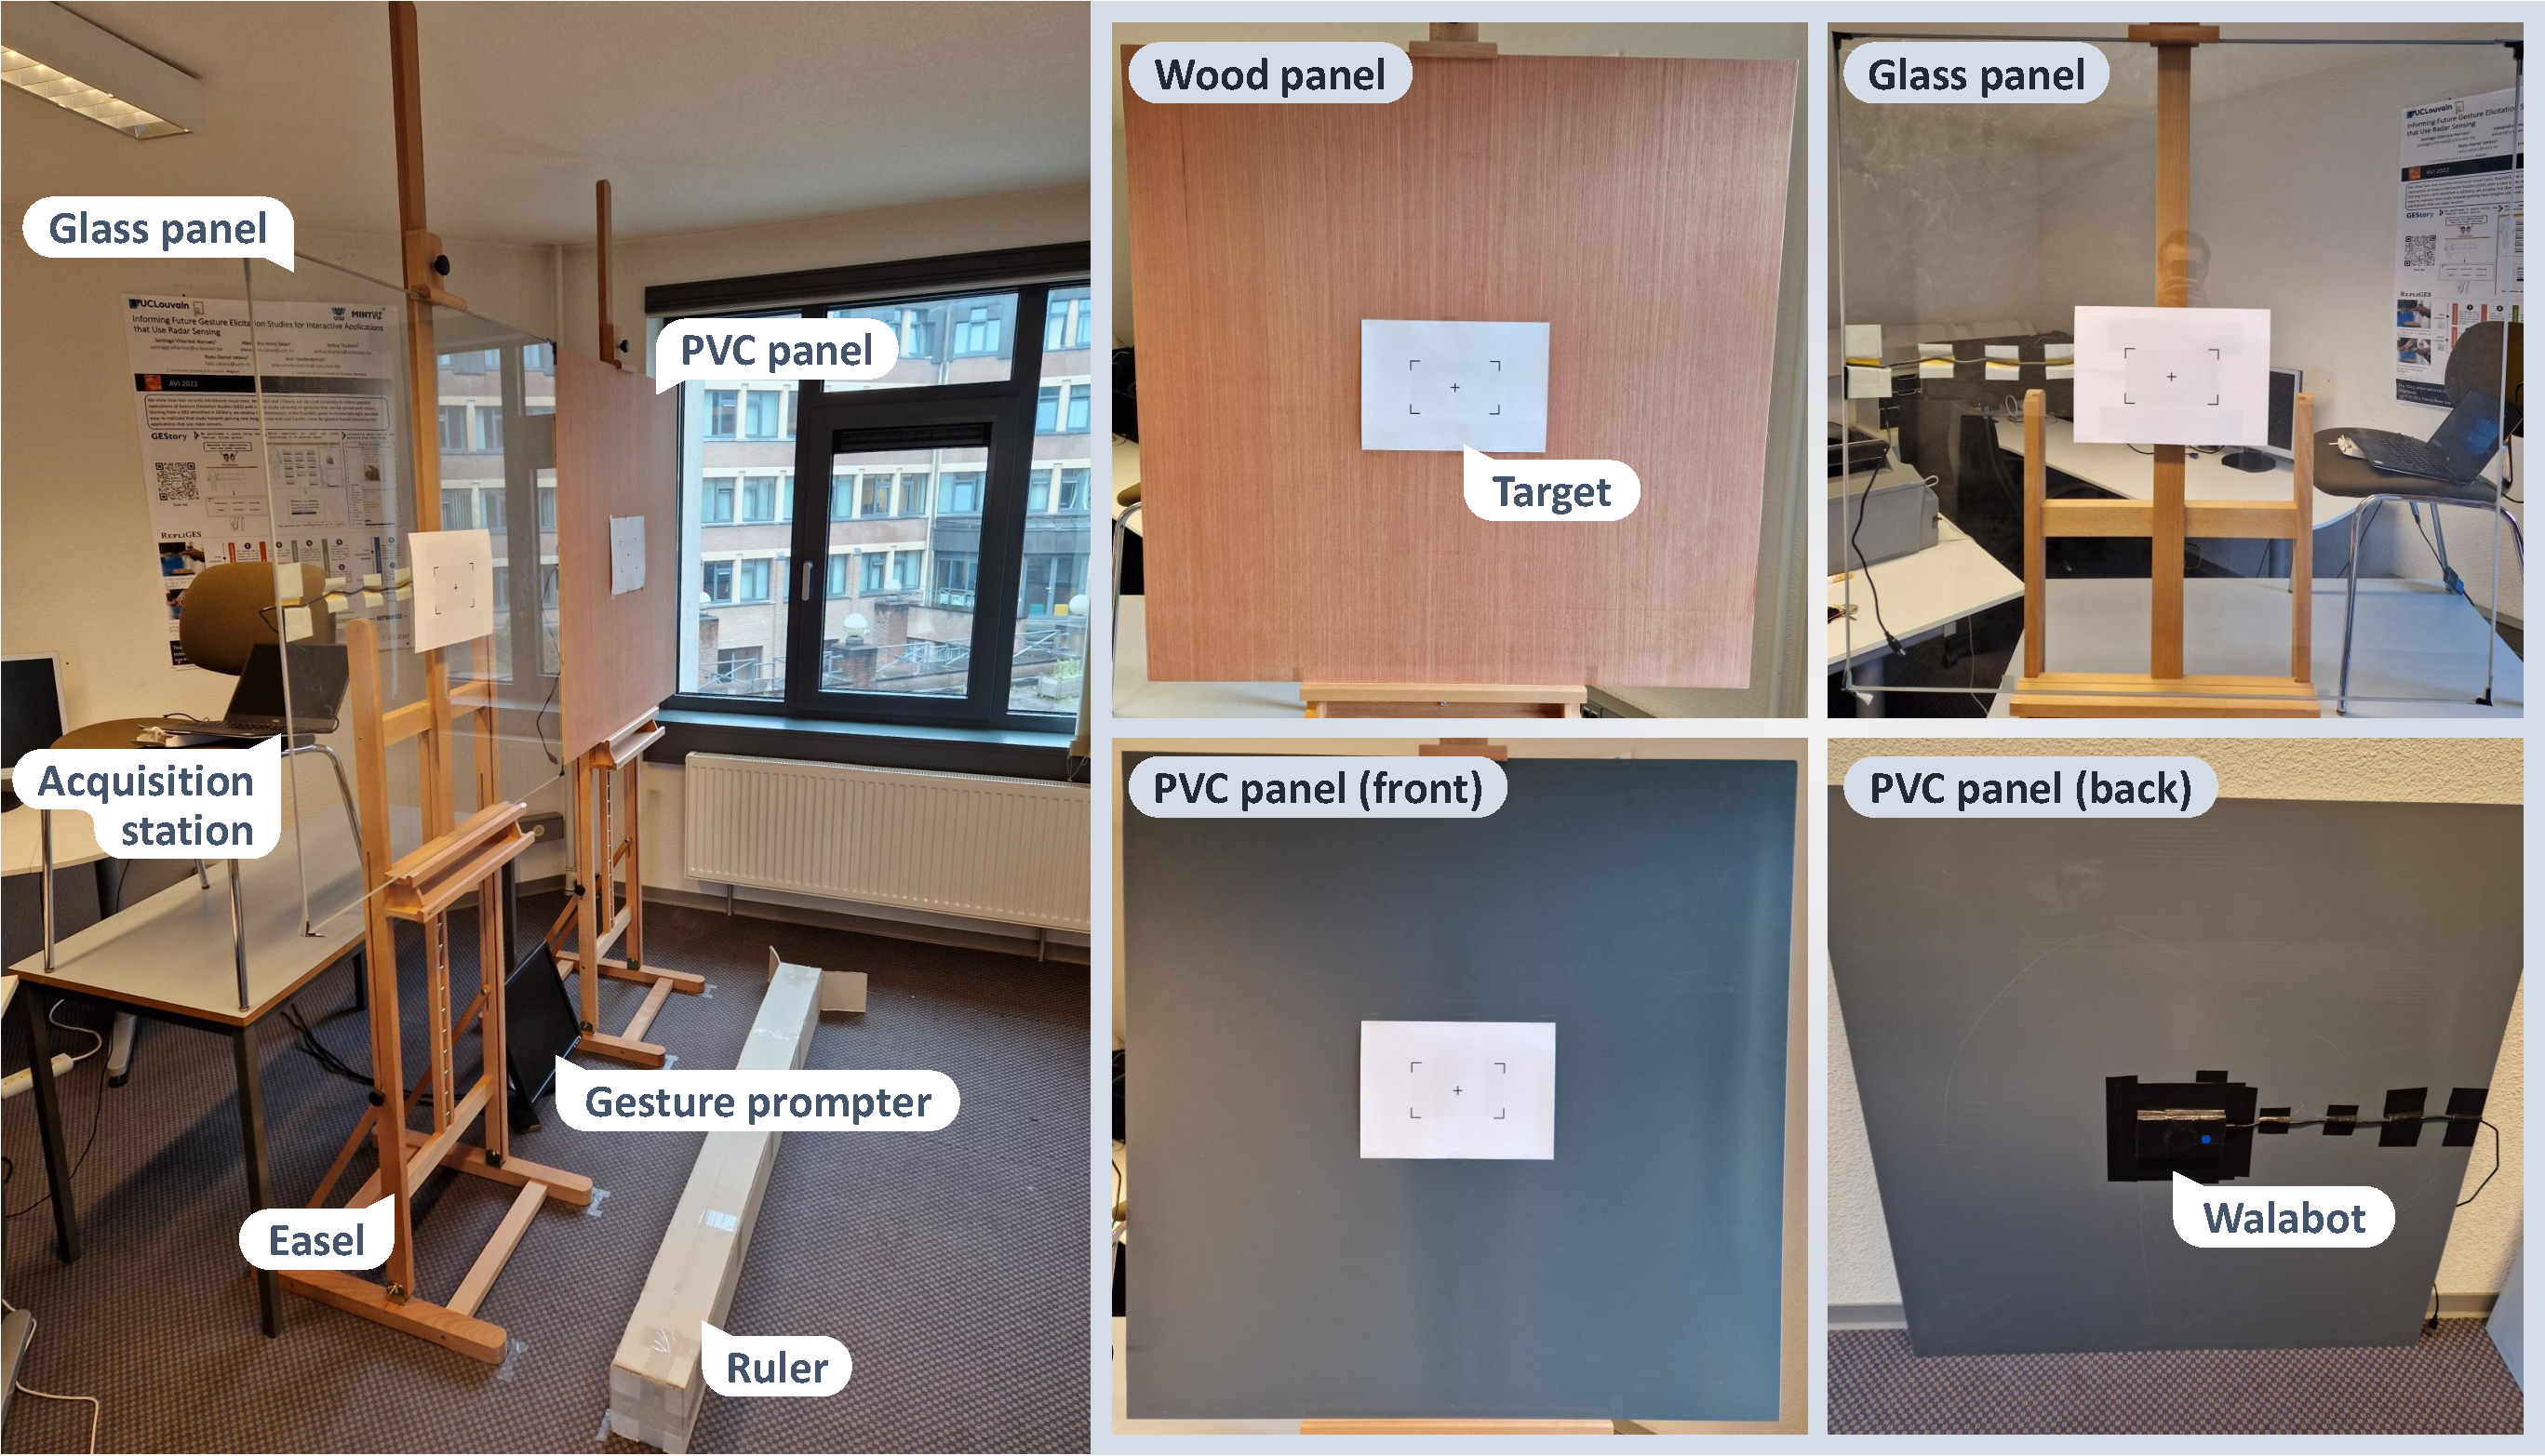
\includegraphics[width=\linewidth]{Figures/RadarExperiments/Datasets/ThroughMaterials/setup-walabot-materials.pdf}
    \vspace{-12pt}
    \caption{Setup used for acquiring the ``through-materials'' datasets.}
    \label{fig:radar-experiments:setup-walabot-materials}
    % \vspace{-8pt}
\end{figure}

Each gesture was performed five times by 20 participants in a controlled environment, resulting in a total of 9 (gestures) $\times$ 20 (participants) $\times$ 5 (repetitions) ${=}$ 900 samples per type of material. The recording procedure was as follows: show the gesture to the participant, then, for each sample, (1) the participant starts with their arms alongside their body, (2) the recording is started, (3) the participant produces the gesture, (4) the participant places their arms back alongside their body, (5) the recording is stopped and the data saved to a text file. This action sequence was repeated for each repetition of each gesture and each material. 

%--------------------------------------------------------------------------------%
\subsection{Data Pre-processing} \label{sec:radar-experiments:data-collection:pre-processing}

\subsubsection{Sensor Calibration}
All radar sensors, \ie the horn and the Walabot with and without material, were calibrated in the GPRLouvain facilities, featuring a 3D positioning system and a 3 m $\times$ 3 m copper plane specifically designed for radar calibration. Each radar system was placed in front of the copper plate and measurements were taken from at least five different distances to compute the characteristic functions of each emitter/receiver pair of antennas (see Section~\ref{sec:radar-challenges:mathematical-theory:characteristic-functions}). Using more than five distances results in an overdetermined system of equations, thus enhancing the calibration precision.
The custom radar and the Walabot were attached to the 3D positioning system to simplify accurate distance measurements (\fig~\ref{fig:radar-experiments:calibration:horn} and~\ref{fig:radar-experiments:calibration:walabot}). The Walabot with wood, PVC, and glass were moved manually as they were too heavy for the system (\fig~\ref{fig:radar-experiments:calibration:material}).
\begin{figure}[t]
    \centering
    \begin{subfigure}{.32\linewidth}
        \centering
        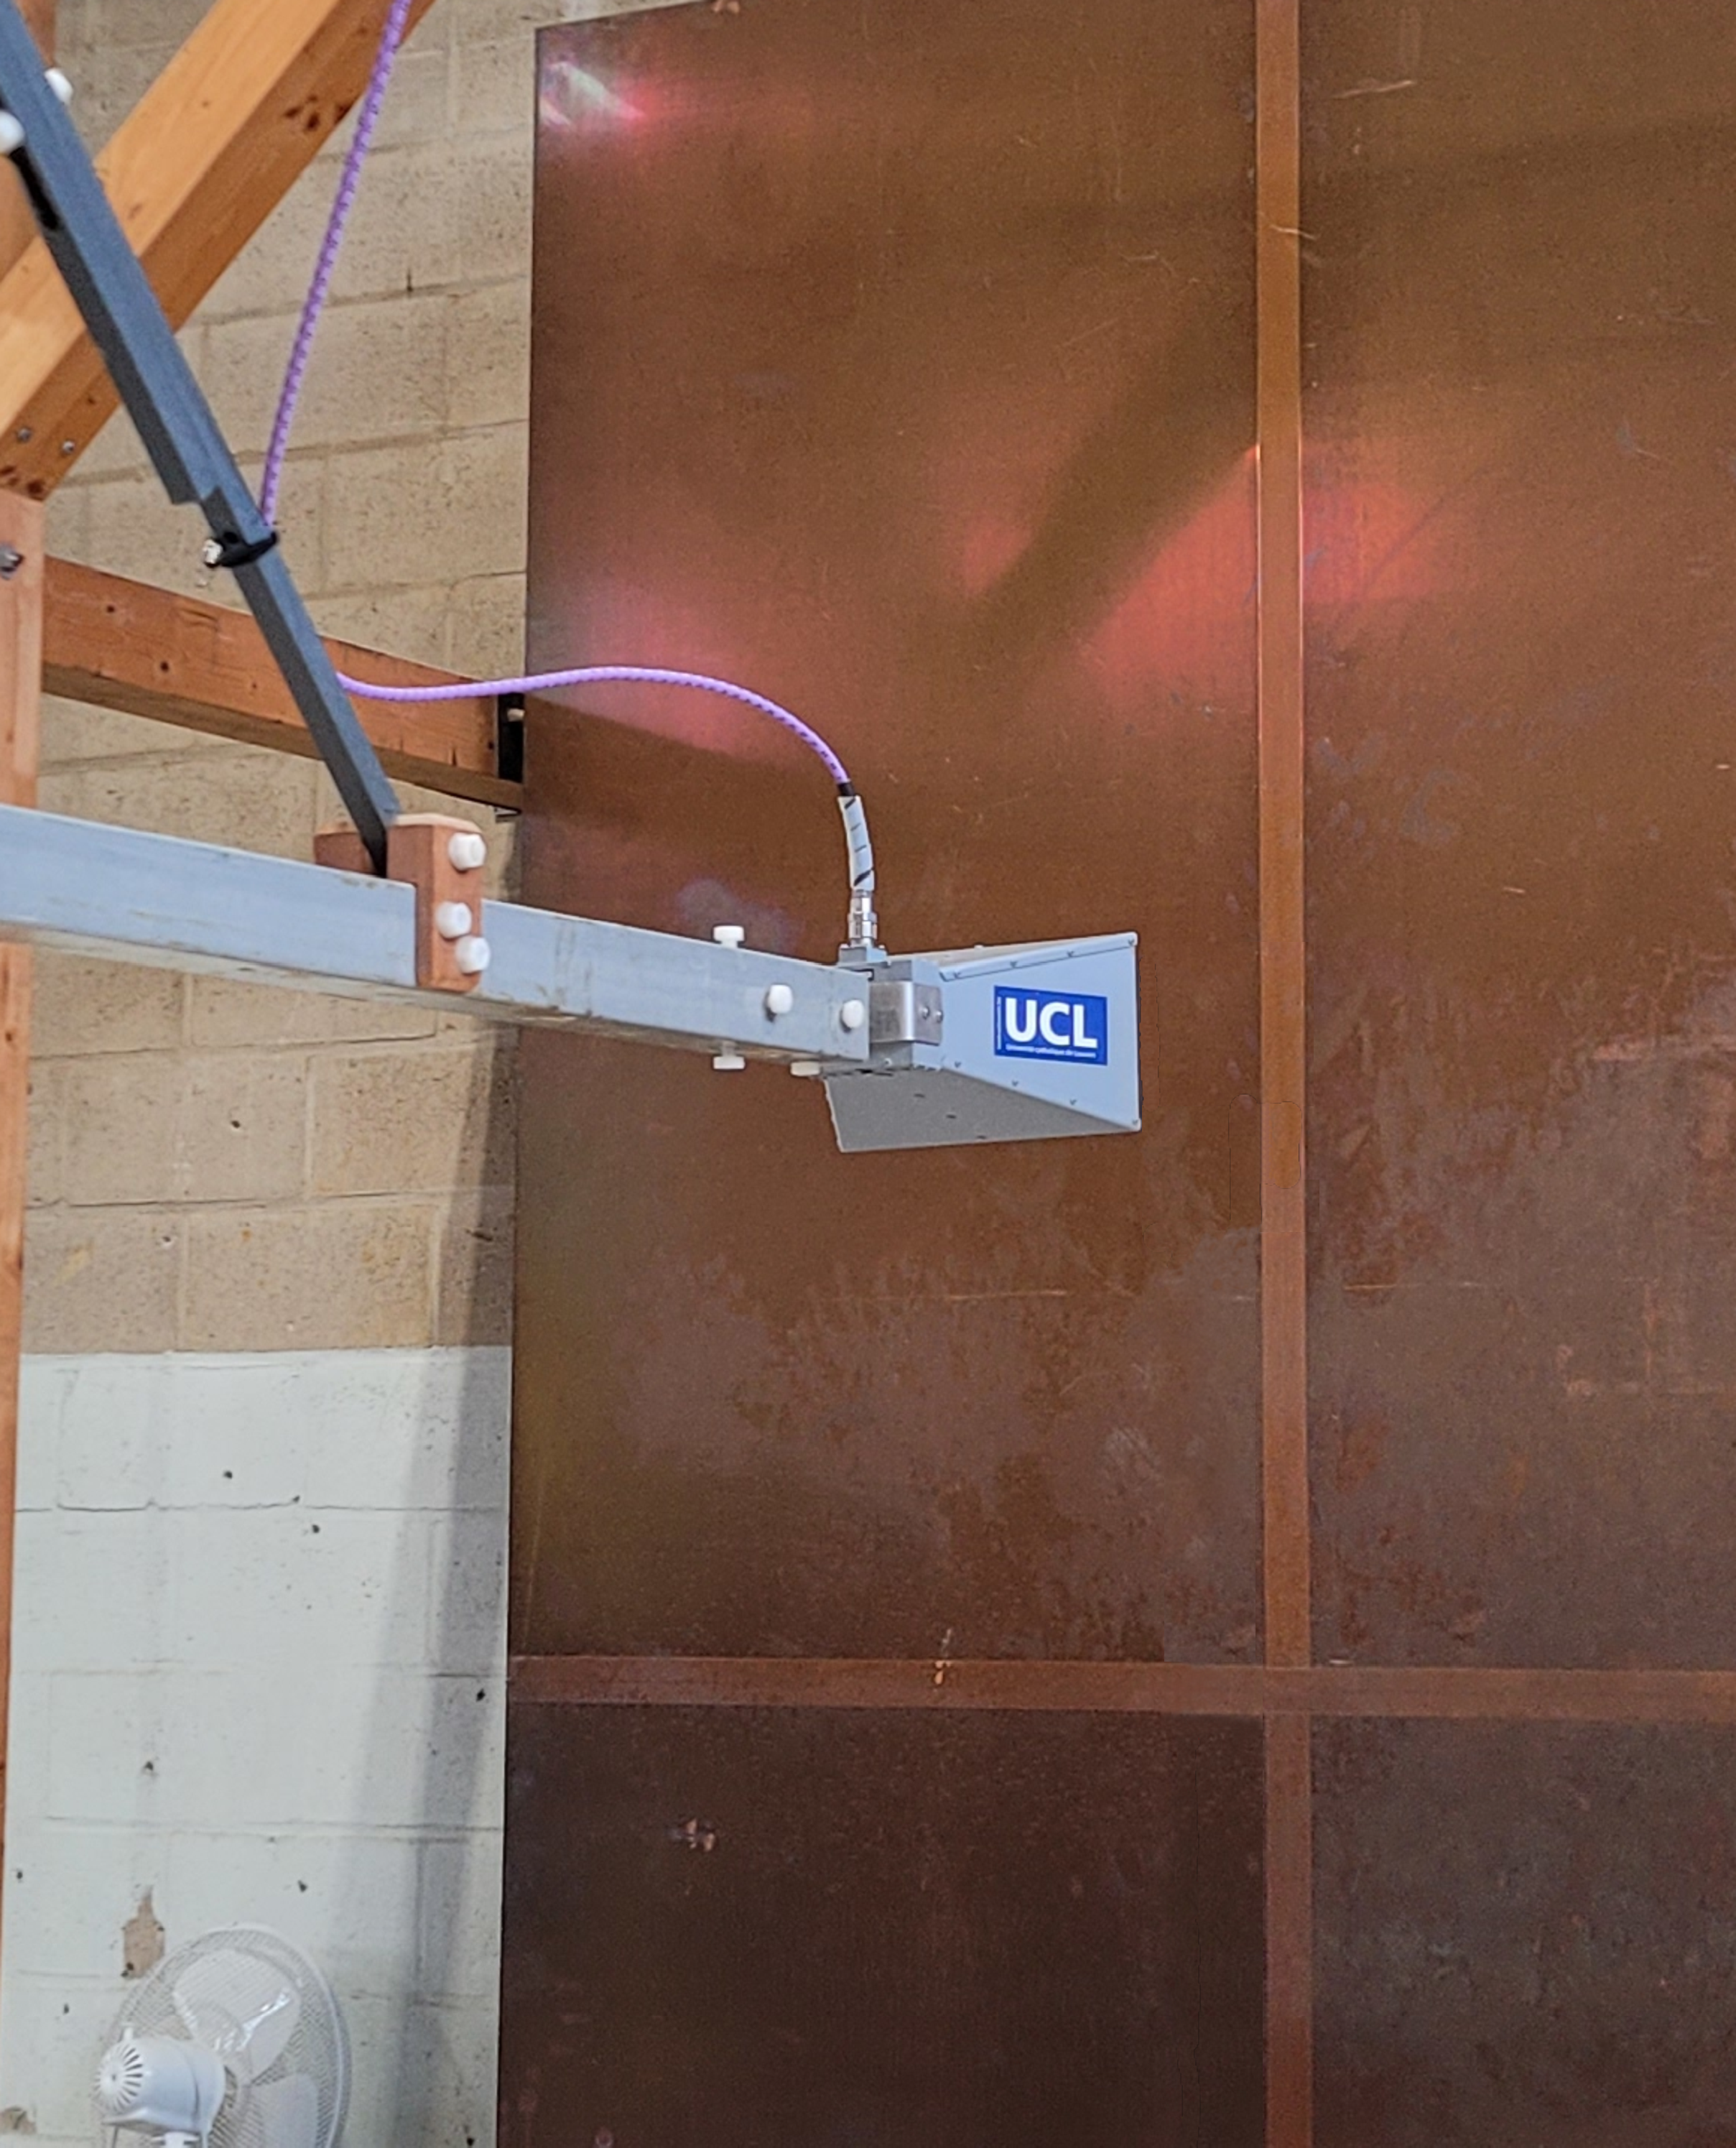
\includegraphics[width=\linewidth,trim={0 2.3cm 0 0},clip]{Figures/RadarExperiments/Calibration/horn-calibration.pdf}
        \captionsetup{width=.99\linewidth}
        \caption{Horn calibration.}
        \label{fig:radar-experiments:calibration:horn}
    \end{subfigure}
    \begin{subfigure}{.32\linewidth}
        \centering
        \includegraphics[width=\linewidth]{Figures/RadarExperiments/Calibration/walabot-calibration.pdf}
        \captionsetup{width=.99\linewidth}
        \caption{Walabot calibration.}
        \label{fig:radar-experiments:calibration:walabot}
    \end{subfigure}
    \begin{subfigure}{.33\linewidth}
        \centering
        \includegraphics[width=\linewidth,trim={0 0 0 0.85cm},clip]{Figures/RadarExperiments/Calibration/wood-calibration.pdf}
        \captionsetup{width=.99\linewidth}
        \caption{Walabot+wood calibration.}
        \label{fig:radar-experiments:calibration:material}
    \end{subfigure}

    \caption{Calibration process of the different radar systems.}
    \label{fig:radar-experiments:calibration}
\end{figure}

\subsubsection{Pipeline Stages}
We processed the radar signals from each dataset with our processing pipeline described in Chapter~\ref{chap:radar-challenges}, which we configured as follows: 
\begin{enumerate}[label=(\alph*)]
    \item \textit{Raw data capture}: all twelve antenna pairs of the Walabot recorded data at about 40 frames per second.
    \item \textit{Radar source \& antenna effects removal}: each antenna pair of the Walabot was calibrated as described in the previous section. The resulting model was applied to each antenna pair to remove the effects of the radar source and antennas.
    \item \textit{Background scene removal}: the second frame of each gesture was subtracted from its other frames.
    \item \textit{Time gating}: the pipeline ignored all reflections received more than 5 ns after the radar signal was emitted, corresponding to approximately 75 cm.
    \item \textit{Full-wave inversion}: the inversion process used a LUT containing 351 permittivity values (between 1 and 8) and 750 distance values (from 1 mm to 75 cm).
    \item \textit{Filtering}: distance and permittivity values were discarded and replaced with default values ($d$ = 75 cm, $\epsilon_{r,e}$=1.0) when the estimated permittivity was lower than 1.1, indicating a hand was not detected in front of the radar. A moving median filter was then applied to the resulting data with a window of size 8. Compared to a moving average, the moving median filter is less sensitive to outliers.
\end{enumerate}
Data from stages a, b, c, and d could be exported in the frequency and time domains.


%================================================================================%
\section{Experiment 1: Sensors and Antenna Subsets} \label{sec:radar-experiments:sensors}
%--------------------------------------------------------------------------------%
\subsection{Aims} \label{sec:radar-experiments:sensors:aims}
This first experiment investigates the performance of three sensors on the ``sensors comparison'' dataset (Section~\ref{sec:radar-experiments:data-collection:datasets:sensors}), a diverse set of 16 hand gestures produced by one participant. This experiment has three main goals:
\begin{enumerate}
    \item Compare the performance of the Walabot with the LMC, a popular vision-based sensor, and the horn, a custom high-end radar.
    \item Evaluate the efficacy of four stages from our signal-processing pipeline (Chapter~\ref{chap:radar-challenges}), namely raw data capture, background scene removal, full-wave inversion, and filtering.
    \item Identify the best-performing sets of pairs of Walabot antennas.
\end{enumerate}

%--------------------------------------------------------------------------------%
\subsection{Protocol} \label{sec:radar-experiments:sensors:protocol}
This experiment consisted of four studies, each following a similar protocol, albeit with slight variations.
%
The \ql testing tool (Chapter~\ref{chap:quantumleap-testing}) was configured with Taranta \etal's Jackknife~\cite{Taranta:2017}, a 1-NN gesture recognizer that can accommodate different data types, works with as few as one training template per class, and is fast to train and execute. We chose to work with an existing recognizer, as implementing the best-performing algorithm for (radar) gesture recognition was outside of the scope of this thesis. However, other algorithms (\eg deep-learning-based) could be used in conjunction with \ql and our data processing pipeline to achieve better performance. Jackknife was set up with its default settings for the inner product distance measure. 
%
The performance of Jackknife on data from each sensor was evaluated following a leave-one-out cross-validation (LOOCV) procedure in a user-dependent and single-dataset scenario (see \tab~\ref{tab:quantumleap-testing:testing-procedures} for a detailed description of the procedure). 
The total number of training templates per trial is 79 (four to five per gesture class), as one of the 80 templates is put aside for testing.
The \textit{recognition rate}, \textit{execution time}, and a \textit{confusion matrix} were computed by \ql for each combination of the studied variables (\eg the number of training templates).
All the tests were run on a laptop with an Intel i7-10875H CPU and 32GB of DDR4 RAM running Windows 10.

We conducted a similar experiment in a previous paper~\cite{Sluyters:2022:IUI} using a train-test-split (TTS) procedure. This experiment addresses some of the limitations of this paper, including the different recording procedures between the LMC+Walabot and LMC+Horn sessions and the fact that Walabot gestures were recorded with only half of the available antenna pairs.


\subsubsection{LMC} \label{sec:radar-experiments:sensors:protocol:lmc}
This first study evaluates the accuracy of Jackknife on the raw LMC data from the LMC+Horn and LMC+Walabot sessions, following the protocol described at the start of Section~\ref{sec:radar-experiments:sensors:protocol}. The study is within-factors with three independent variables:
\begin{enumerate}
    \item \custominlinehighlight{Recording Session}: nominal variable with two conditions, representing the recording session of the training data: LMC+Walabot, and LMC+Horn.
    % \item \custominlinehighlight{Number of Templates}: numerical variable with 3 conditions, representing the number of templates per gesture class used to train the recognizer: $T{=}\{1,2,4\}$.
    \item \custominlinehighlight{Number of Sampling Points}: numerical variable with 37 values representing the number of points per gesture template: $N{=}\{x\in\mathbb{N} \mid 4 \leq x \leq 40\}$.
    \item \custominlinehighlight{Number of Joints}: numerical variable with three conditions (\fig \ref{fig:radar-experiments:lmc-joints}), representing the number of joints used to train the recognizer: $J{\in}\{6,11,16\}$. 
\end{enumerate}
Each gesture sample consists of a sequence of frames, where each frame has two elements: a timestamp and a vector of length $3 \times J$ resulting from the concatenation of the 3D coordinates ($x$,$y$,$z$) of the selected joints. 

\begin{figure*}[tb]
    \centering
    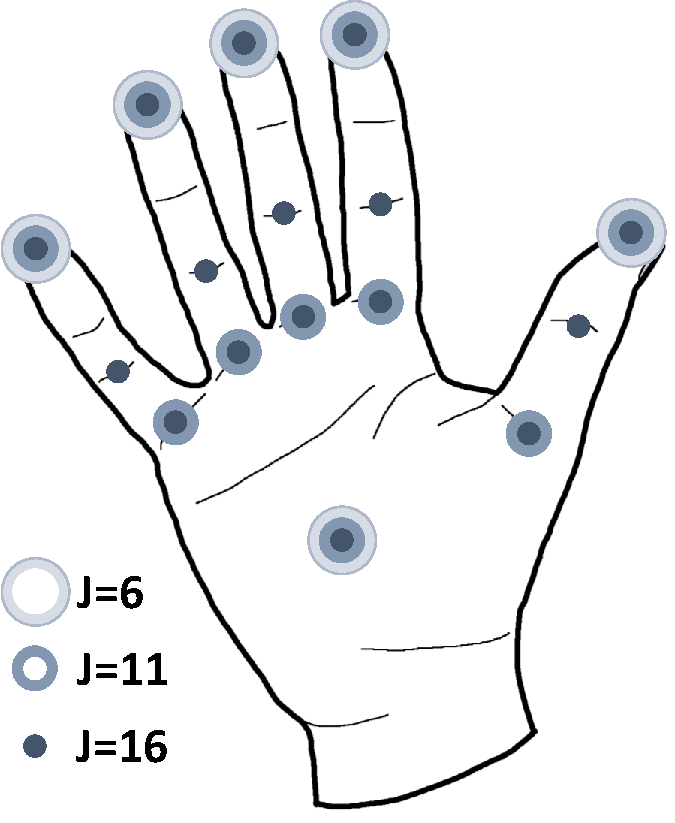
\includegraphics[width=.35\linewidth]{Figures/RadarExperiments/Sensors/lmc-joints.pdf}
    % \vspace{-12pt}
    \caption{Joints used in each condition $J{\in}\{6,11,16\}$.}
    \label{fig:radar-experiments:lmc-joints}
    % \vspace{-14pt}
\end{figure*}

\subsubsection{Horn} \label{sec:radar-experiments:sensors:protocol:horn}
This second study evaluates the accuracy of Jackknife on the Horn data from four stages of the radar data processing pipeline. The study is within-factors with two independent variables:
\begin{enumerate}
    \item \custominlinehighlight{Processing Stage}: nominal variable with four conditions, representing the processing stage of the training data: raw data capture, background scene removal, full-wave inversion, and filtering.
    % \item \custominlinehighlight{Number of Templates}: numerical variable with 3 conditions, representing the number of templates per gesture class used to train the recognizer: $T{=}\{1,2,4\}$.
    \item \custominlinehighlight{Number of Sampling Points}: same as the first study.
\end{enumerate}
Each gesture template consists of a sequence of frames, where each frame contains two elements: (1) a timestamp and (2) a vector containing the radar data at that instant. In the inversion and filtering stages, the vector contains two elements: the distance and apparent permittivity evaluated at that instant. In the other stages, the vector (length $2 \times 89$) contains the real and imaginary parts of the frequency-domain radar signal (89 frequencies). 


\subsubsection{Walabot} \label{sec:radar-experiments:sensors:protocol:walabot}
The last two studies were conducted on the Walabot data.
%
The third study evaluates the impact of the selected set of antenna pairs on the accuracy of Jackknife at four stages of the radar data processing pipeline. The number of sampling points is fixed to $N{=}16$. The study is within-factors with two independent variables:
\begin{enumerate}
    \item \custominlinehighlight{Processing Stage}: same as the second study.
    % \item \custominlinehighlight{Number of Templates}: numerical variable with 3 conditions, representing the number of templates per gesture class used to train the recognizer: $T{=}\{1, 2, 4\}$.
    \item \custominlinehighlight{Antenna Pairs}: nominal variable with 127 conditions, representing all the possible combinations of non-redundant antenna pairs (excluding the empty set) and the set of all antenna pairs: $\splitatcommas{AP=\{(1), (2), (3), (6), (8), (9), (1, 2), ..., (2, 3, 6, 8, 9), (1, 2, 3, 6, 8, 9)\} \cup \{(4), (5), (7), (10), (11), (12), (4, 5), ..., (5, 7, 10, 11, 12), (4, 5, 7, 10, 11, 12)\} \cup \{(1, 2, 3, 4, 5, 6, 7, 8, 9, 10, 11, 12)\}}$.
\end{enumerate}
%
The fourth study investigates the impact of the number of sampling points on the accuracy of Jackknife for the three best-performing sets of antenna pairs of each processing stage (determined in the previous study).
This study is also within-factors, with three independent variables:
\begin{enumerate}
    \item \custominlinehighlight{Processing Stage}: same as the first study.
    % \item \custominlinehighlight{Number of Templates}: same as the first study.
    \item \custominlinehighlight{Number of Sampling Points}: same as the first study.
    \item \custominlinehighlight{Antenna Pairs}: nominal variable with 18 conditions, representing the three best-performing sets of antenna pairs determined in the first study, all single antenna pairs, the two largest sets of non-redundant antenna pairs, and the set of all antenna pairs. For instance, for the ``filtering'' processing stage, $\splitatcommas{AP=\{(1, 2, 6, 8, 9), (1, 2, 8, 9), (4, 7, 10, 11, 12)\} \cup \{(1), (2), ..., (11), (12)\} \cup \{(1, 2, 3, 6, 8, 9), (4, 5, 7, 10, 11, 12), (1, 2, 3, 4, 5, 6, 7, 8, 9, 10, 11, 12)\}}$.    
    % best-performing combinations of antenna pairs determined in the first study. For instance, for the ``raw data capture'' processing stage, $\splitatcommas{AP=\{(4, 5, 7, 11), (4, 7, 11), (1, 2, 3, 4, 5, 6, 7, 8, 9, 10, 11, 12)\}}$.
\end{enumerate}
In both studies, a gesture template consists of a sequence of frames, each containing two elements: (1) a timestamp and (2) a vector with the radar data at that instant. In the inversion and filtering steps, the vector (length $2 \times AP$) is the concatenation of the distance and permittivity values retrieved from all the antenna pairs. In the other stages, the vector (length $2 \times 34 \times AP$) results from the concatenation of the real and imaginary parts of the frequency-domain radar signal (34 frequencies) from the selected pairs of antennas.


%--------------------------------------------------------------------------------%
\subsection{Results} \label{sec:radar-experiments:sensors:results}

\subsubsection{LMC} \label{sec:radar-experiments:sensors:results:lmc}
\fig~\ref{fig:radar-experiments:sensors:lmc-samples} depicts the evolution of accuracy with respect to the number of sampling points on data from the LMC+Horn and LMC+Walabot sessions.
%
The best configurations achieved 92.5\% accuracy for both the LMC+Horn ($N{=}10$, $J{=}6$) and LMC+Walabot ($N{=}27$, $J{=}11$) sessions.
Execution time was short at 0.3 and 0.8 ms, respectively, and stayed under 1 ms in most configurations. Overall, the execution time increased with the number of sampling points and joints.
%
In general, average accuracy dropped sharply with $N{<}7$ and plateaued around 90\% for higher values of $N$. However, accuracy was less stable with respect to $N$ for the LMC+Walabot session.

\begin{figure}[htbp]
    \begin{subfigure}{.49\textwidth}
        \centering
        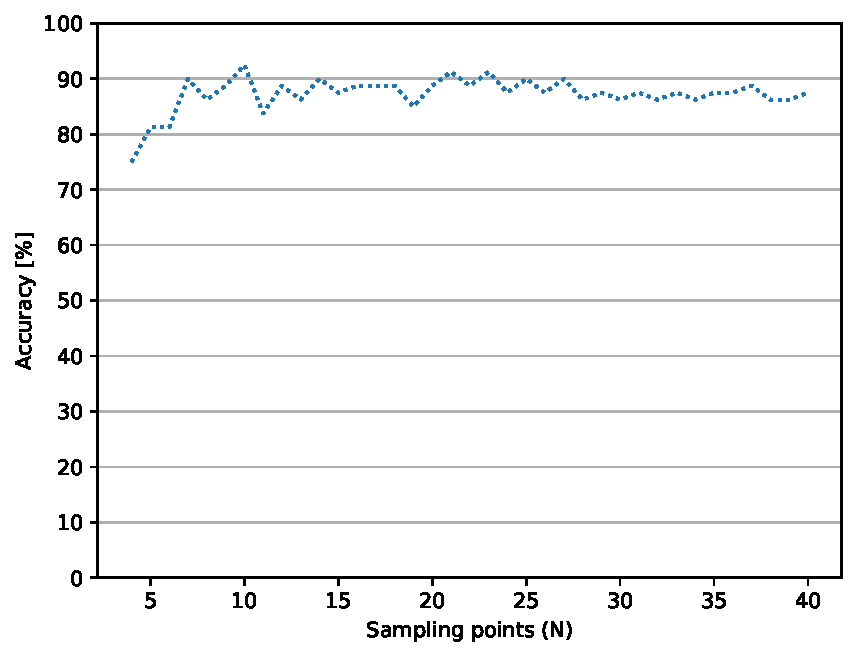
\includegraphics[width=.99\linewidth]{Figures/RadarExperiments/Datasets/SensorsComparison/LMC/LMC+Horn-samples-6.pdf}
        \vspace{-15pt}
        \captionsetup{width=.99\linewidth}
        \caption{6 joints (Horn).}
        \label{fig:radar-experiments:sensors:lmc-samples:horn-6}
    \end{subfigure}
    \begin{subfigure}{.49\textwidth}
        \centering
        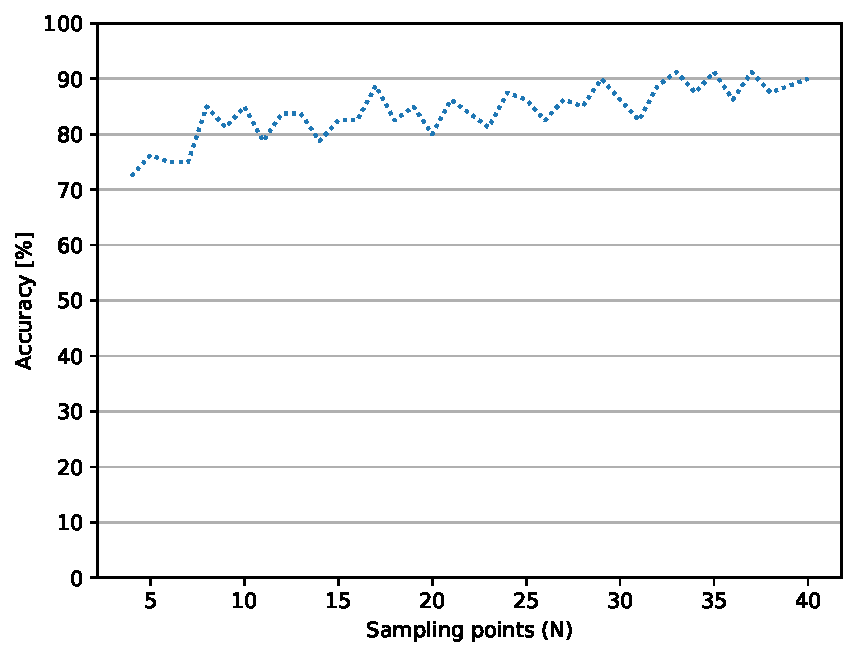
\includegraphics[width=.99\linewidth]{Figures/RadarExperiments/Datasets/SensorsComparison/LMC/LMC+Walabot-samples-6.pdf}
        \vspace{-15pt}
        \captionsetup{width=.99\linewidth}
        \caption{6 joints (Walabot).}
        \label{fig:radar-experiments:sensors:lmc-samples:walabot-6}
    \end{subfigure}

    \begin{subfigure}{.49\textwidth}
        \centering
        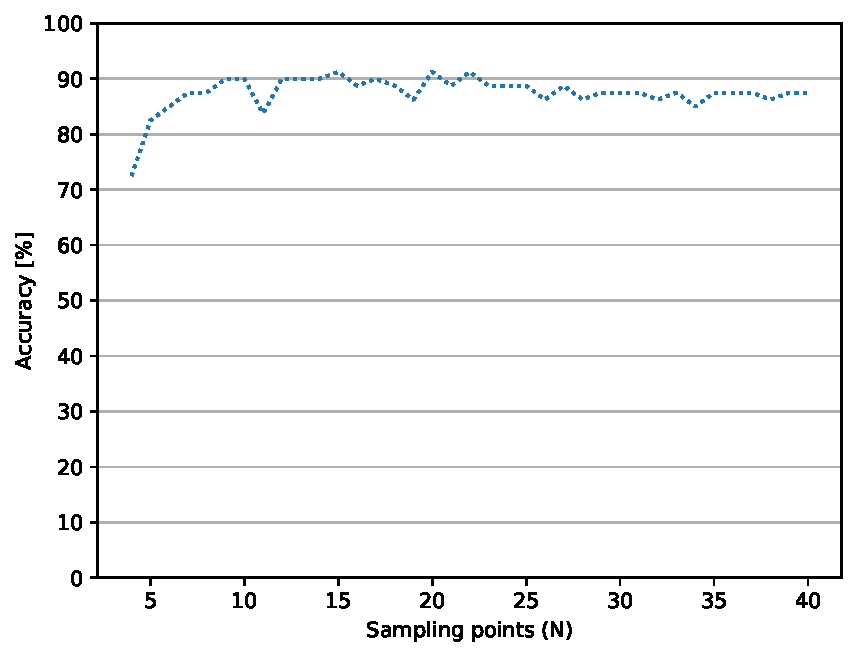
\includegraphics[width=.99\linewidth]{Figures/RadarExperiments/Datasets/SensorsComparison/LMC/LMC+Horn-samples-11.pdf}  
        \vspace{-15pt}
        \captionsetup{width=.99\linewidth}
        \caption{11 joints (Horn).}
        \label{fig:radar-experiments:sensors:lmc-samples:horn-11}
    \end{subfigure}
    \begin{subfigure}{.49\textwidth}
        \centering
        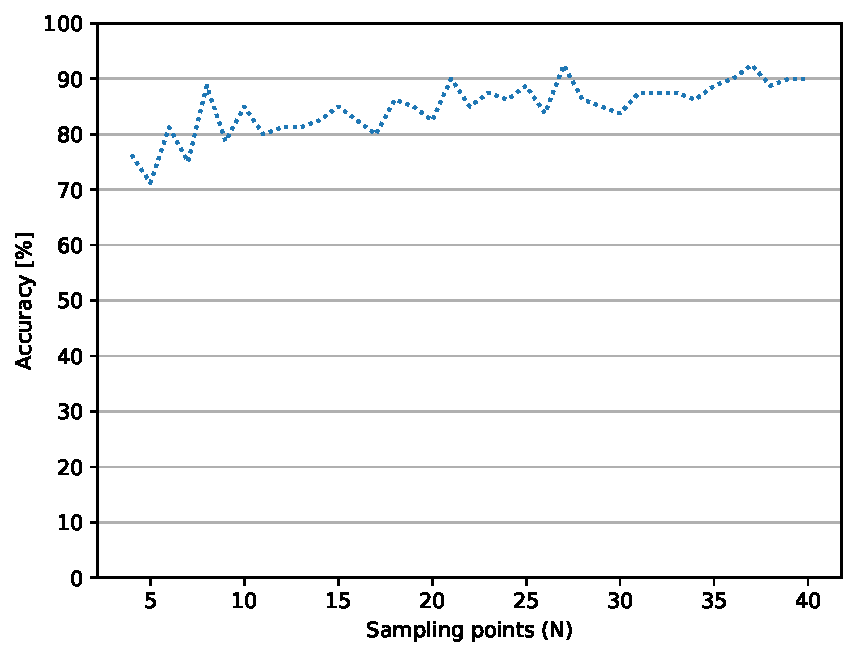
\includegraphics[width=.99\linewidth]{Figures/RadarExperiments/Datasets/SensorsComparison/LMC/LMC+Walabot-samples-11.pdf}  
        \vspace{-15pt}
        \captionsetup{width=.99\linewidth}
        \caption{11 joints (Walabot).}
        \label{fig:radar-experiments:sensors:lmc-samples:walabot-11}
    \end{subfigure}

    \begin{subfigure}{.49\textwidth}
        \centering
        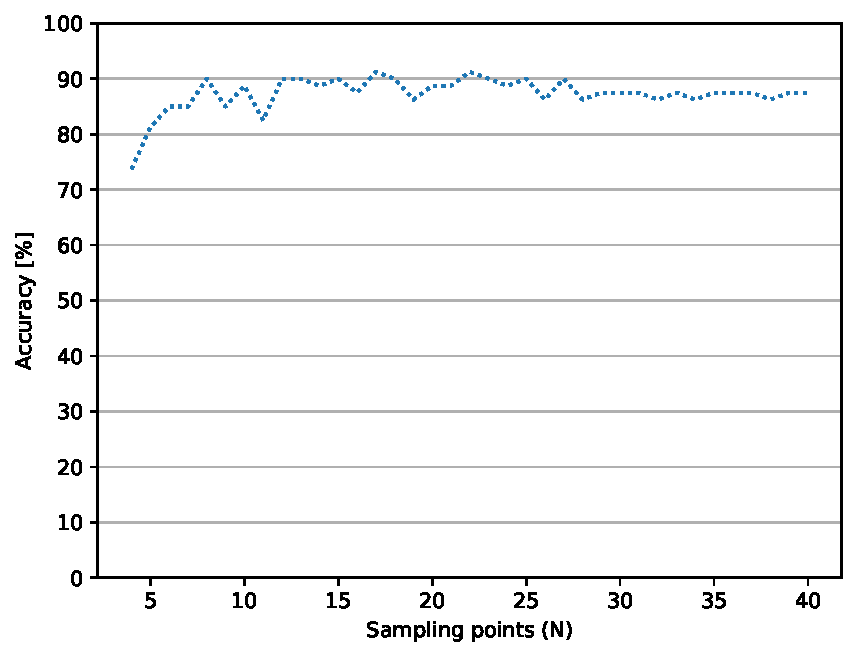
\includegraphics[width=.99\linewidth]{Figures/RadarExperiments/Datasets/SensorsComparison/LMC/LMC+Horn-samples-16.pdf}  
        \vspace{-15pt}
        \captionsetup{width=.99\linewidth}
        \caption{16 joints (Horn).}
        \label{fig:radar-experiments:sensors:lmc-samples:horn-16}
    \end{subfigure}
    \begin{subfigure}{.49\textwidth}
        \centering
        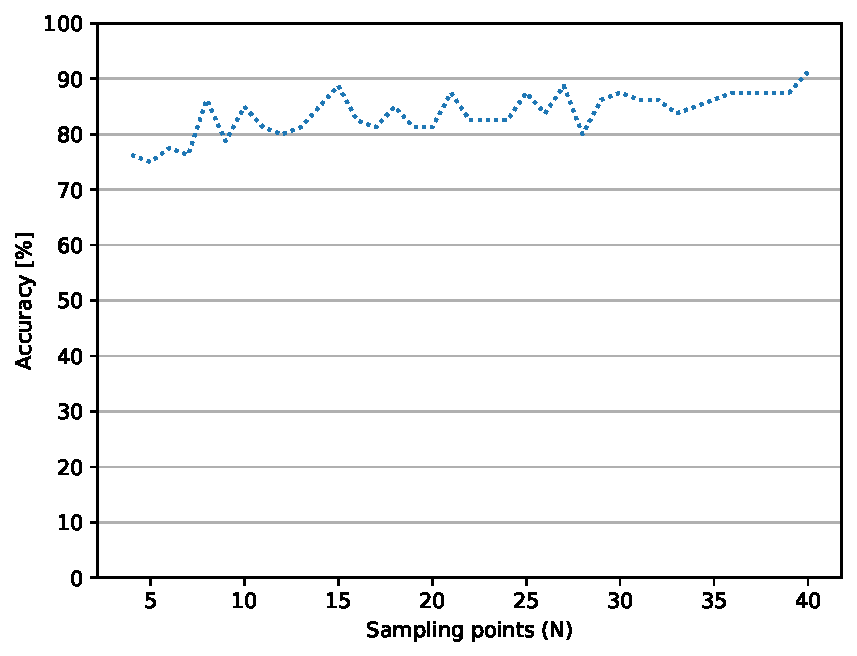
\includegraphics[width=.99\linewidth]{Figures/RadarExperiments/Datasets/SensorsComparison/LMC/LMC+Walabot-samples-16.pdf}  
        \vspace{-15pt}
        \captionsetup{width=.99\linewidth}
        \caption{16 joints (Walabot).}
        \label{fig:radar-experiments:sensors:lmc-samples:walabot-16}
    \end{subfigure}
    % \vspace{-8pt}
    \caption{The accuracy of Jackknife with respect to the number of sampling points on the LMC data of the LMC+Horn (left) and LMC+Walabot (right) sessions.}
    \label{fig:radar-experiments:sensors:lmc-samples}
\end{figure}


\fig~\ref{fig:radar-experiments:sensors:lmc-confusion} shows the confusion matrices for the best configurations of Jackknife on data from the LMC+Horn and LMC+Walabot sessions. 
%
In general, smaller-scale hand gestures, including ``extend one/two/three/four fingers'' (gestures d, e, f, g) were less accurately identified by the LMC, which could have been caused by self-occlusion, where some part of the hand (\eg the fingers) was occluded by another part of the hand (\eg the hand palm). The placement of the LMC on a desk under the participant's hands meant that it could not always correctly identify the exact position of the fingers, thus causing confusion between these gestures.
%
We also observed some confusion between the ``swipe left'' and ``barrier'' gestures (gestures i and u), between ``open hand'' and ``push palm'' (gestures a and p), and between ``extend four fingers'' and ``swipe down'' (gestures g and k). Confusion in all of these cases can be explained by some similarity in the motion of the gestures. For instance, the end of ``extend four fingers'' looks similar to swiping down.
%
Compared to a similar experiment described in our previous paper~\cite{Sluyters:2022:IUI}, we did not observe confusion between the ``open hand'', ``close hand'', and ``open then close hand'' gestures from the LMC+Walabot session, which seems to confirm our hypothesis that the confusion was caused by the fixed length of the recordings.

% % Horn
% 92.5\%, 0.3ms ($N{=}10$, $J{=}6$)
% 91.3\%, 0.5ms ($N{=}15$, $J{=}11$)
% 91.3\%, 0.7ms ($N{=}17$, $J{=}16$)

% % Walabot
% 91.3\%, 0.9ms ($N{=}33$, $J{=}6$)
% 92.5\%, 0.8ms ($N{=}27$, $J{=}11$)
% 91.3\%, 1.5ms ($N{=}40$, $J{=}16$)

\begin{figure}[t]
    \begin{subfigure}{.49\textwidth}
        \centering
        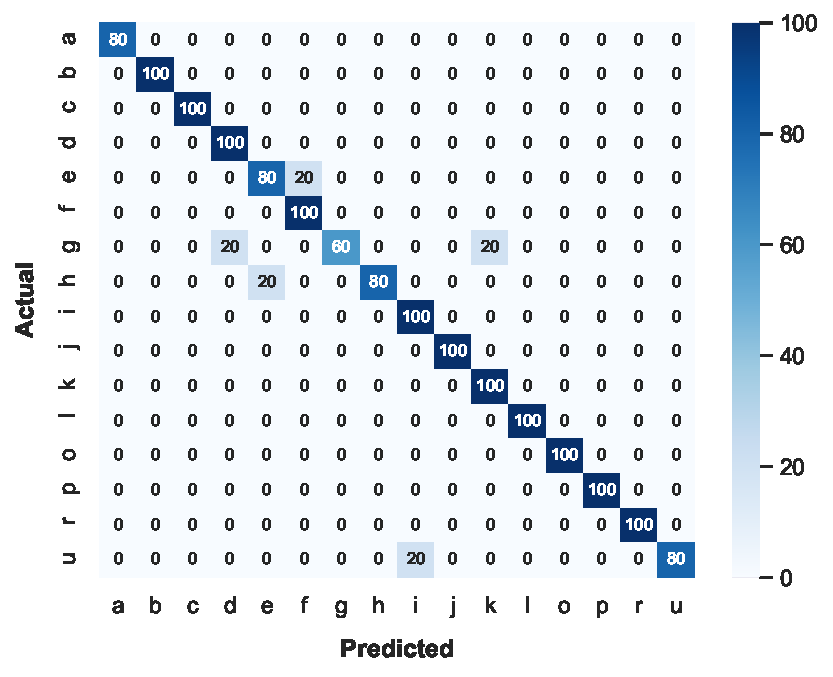
\includegraphics[width=.99\linewidth]{Figures/RadarExperiments/Datasets/SensorsComparison/LMC/LMC+Horn-confusion-6.pdf}  
        \vspace{-16pt}
        \captionsetup{width=.99\linewidth}
        \caption{LMC+Horn session ($N{=}10$, $J{=}6$).}
        \label{fig:radar-experiments:sensors:lmc-confusion:horn}
    \end{subfigure}
    \begin{subfigure}{.49\textwidth}
        \centering
        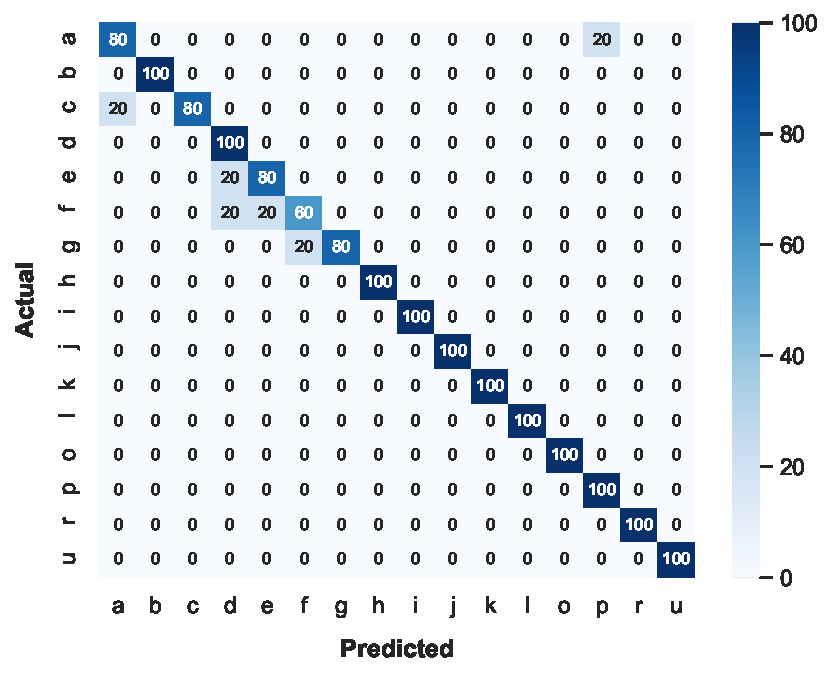
\includegraphics[width=.99\linewidth]{Figures/RadarExperiments/Datasets/SensorsComparison/LMC/LMC+Walabot-confusion-11.pdf}
        \vspace{-16pt}
        \captionsetup{width=.99\linewidth}
        \caption{LMC+Walabot session ($N{=}27$, $J{=}11$).}
        \label{fig:radar-experiments:sensors:lmc-confusion:walabot}
    \end{subfigure}
    \caption{Normalized confusion matrices for the best configuration with LMC data on the LMC+Horn and LMC+Walabot sessions. The values are represented as percentages.}
    \label{fig:radar-experiments:sensors:lmc-confusion}
\end{figure}


\subsubsection{Horn} \label{sec:radar-experiments:sensors:results:horn}
\fig~\ref{fig:radar-experiments:sensors:horn-samples} shows, for the four processing stages, the accuracy of Jackknife with respect to the number of sampling points and training templates. In addition, \fig~\ref{fig:radar-experiments:sensors:horn-confusion} shows the confusion matrix of the best-performing configuration for each stage.


% Raw data
% 93.8\%, 6.0ms ($N{=}28$)
\paragraph{Raw data capture.}
The average accuracy on the raw radar data was already very high and hovered around 90\% with $N{\ge}12$ sampling points, reaching up to 93.8\% for $N{=}28$ (\fig~\ref{fig:radar-experiments:sensors:horn-samples:raw}), with an average execution time of 6.0 ms. Overall, the execution time increased with the number of sampling points. 
%
The corresponding confusion matrix (\fig~\ref{fig:radar-experiments:sensors:horn-confusion:raw}) shows that 11 of the 16 gesture classes were correctly recognized 100\% of the time. The remaining gestures were ``extend three fingers'', ``swipe right'', ``swipe up'', ``draw infinity'', and ``barrier gesture'' (f, h, j, l, u). 
%
In particular, gestures j and l were confused with gesture k (swipe down). They all featured similar hand poses with different trajectories in the plane orthogonal to the direction of the emitted radar signal, which can be difficult to distinguish from a single radar antenna. In that respect, an antenna array such as the Walabot, may be preferable.
%
Similarly, gesture h may have been confused with gesture c (open then close hand) because an open hand positioned off-center from the radar antenna reflects less of the signal and can thus be interpreted as a closed fist right in front of the radar.
%
Finally, the confusion between gestures f and g (extend four fingers) is probably caused by their similar radar cross-sections.

\begin{figure}[tbp]
    \begin{subfigure}{.49\textwidth}
        \centering
        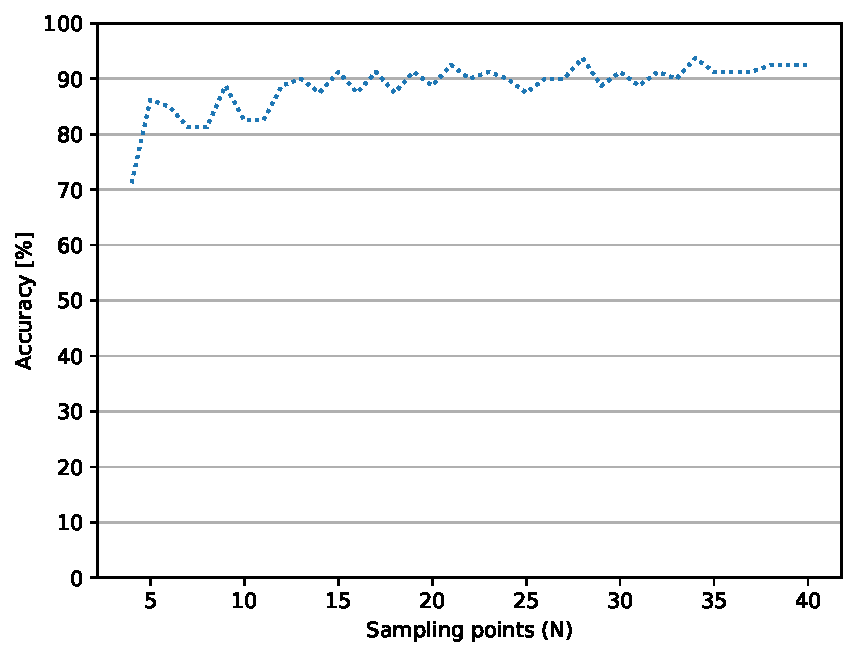
\includegraphics[width=.99\linewidth]{Figures/RadarExperiments/Datasets/SensorsComparison/Horn/samples-raw.pdf}
        \vspace{-15pt}
        \captionsetup{width=.99\linewidth}
        \caption{Raw data capture.}
        \label{fig:radar-experiments:sensors:horn-samples:raw}
    \end{subfigure}
    \begin{subfigure}{.49\textwidth}
        \centering
        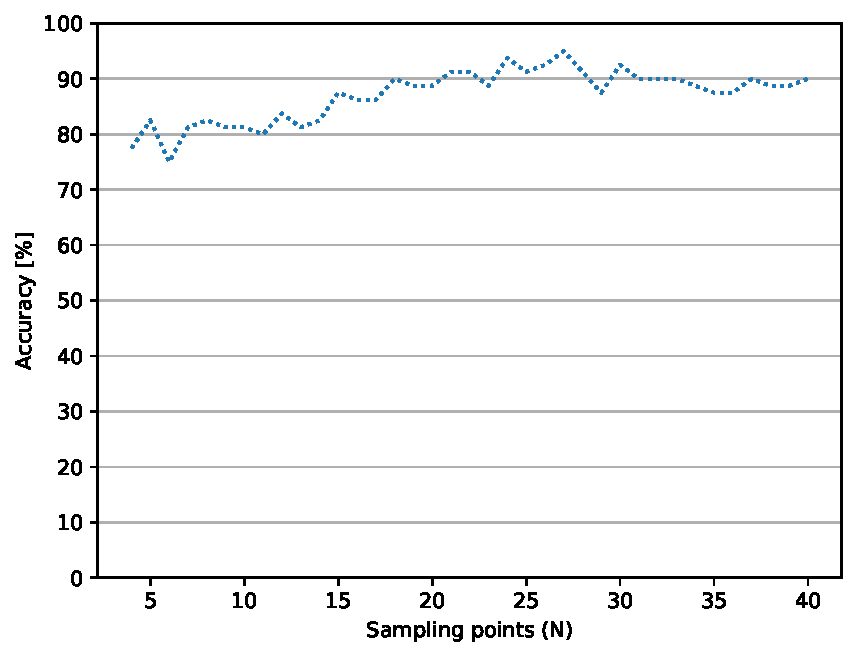
\includegraphics[width=.99\linewidth]{Figures/RadarExperiments/Datasets/SensorsComparison/Horn/samples-bgsub.pdf}  
        \vspace{-15pt}
        \captionsetup{width=.99\linewidth}
        \caption{Background scene removal.}
        \label{fig:radar-experiments:sensors:horn-samples:bgsub}
    \end{subfigure}
    
    \begin{subfigure}{.49\textwidth}
        \centering
        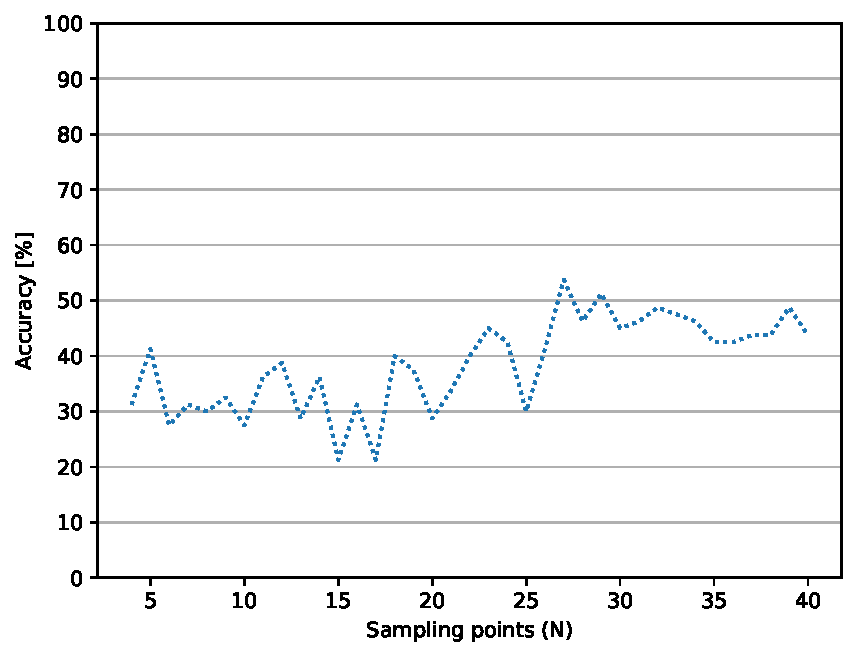
\includegraphics[width=.99\linewidth]{Figures/RadarExperiments/Datasets/SensorsComparison/Horn/samples-inversion.pdf}
        \vspace{-15pt}
        \captionsetup{width=.99\linewidth}
        \caption{Inversion.}
        \label{fig:radar-experiments:sensors:horn-samples:inversion}
    \end{subfigure}
    \begin{subfigure}{.49\textwidth}
        \centering
        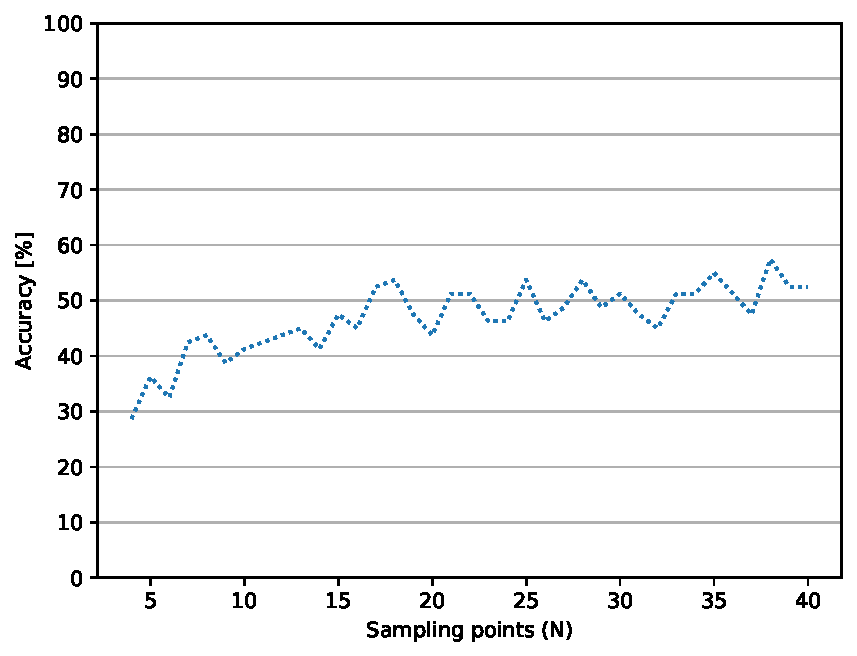
\includegraphics[width=.99\linewidth]{Figures/RadarExperiments/Datasets/SensorsComparison/Horn/samples-filtering.pdf}
        \vspace{-15pt}
        \captionsetup{width=.99\linewidth}
        \caption{Filtering.}
        \label{fig:radar-experiments:sensors:horn-samples:filtering}
    \end{subfigure}
    
    \vspace{-6pt}
    \caption{The accuracy of Jackknife with respect to the number of sampling points with data acquired from the Horn at four different stages of the pipeline.}
    \label{fig:radar-experiments:sensors:horn-samples}
\end{figure}

% Background scene removal
% 95.0\%, 5.8ms ($N{=}27$)
\paragraph{Background scene removal.}
The removal of antenna effects and background subtraction enabled even higher recognition rates, reaching 95.0\% for $N{=}27$ (\fig~\ref{fig:radar-experiments:sensors:horn-samples:bgsub}), with an average execution time of 5.8 ms. The resulting confusion matrix (\fig~\ref{fig:radar-experiments:sensors:horn-confusion:bgsub}) is similar to the confusion matrix obtained on the raw data, with some minor differences that can be explained in the same way. 100\% recognition rate was achieved for 12 of the 16 gesture classes, with the four other gestures being ``extend one finger'', ``swipe right'', ``swipe up'', and ``barrier gesture'' (d, h, j, u).

\begin{figure}[tbp]
    \begin{subfigure}{.49\textwidth}
        \centering
        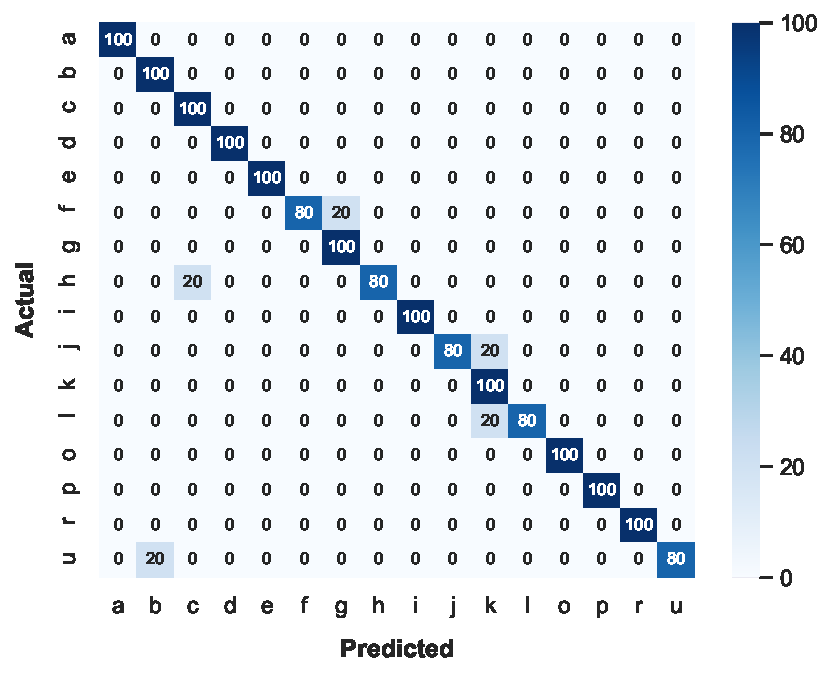
\includegraphics[width=.99\linewidth]{Figures/RadarExperiments/Datasets/SensorsComparison/Horn/confusion-raw.pdf}
        \vspace{-18pt}
        \captionsetup{width=.99\linewidth}
        \caption{Raw data capture ($N{=}28$).}
        \label{fig:radar-experiments:sensors:horn-confusion:raw}
    \end{subfigure}
    \begin{subfigure}{.49\textwidth}
        \centering
        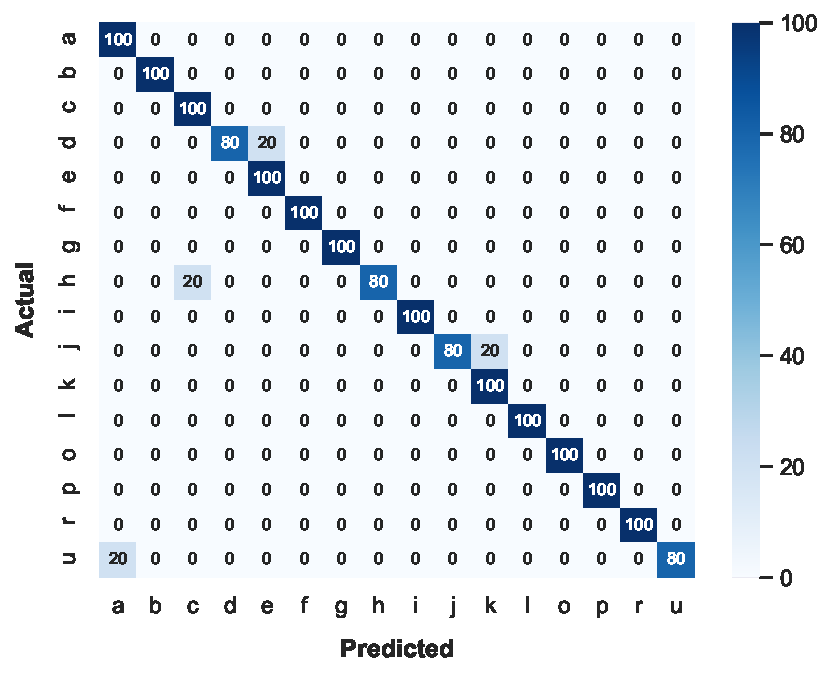
\includegraphics[width=.99\linewidth]{Figures/RadarExperiments/Datasets/SensorsComparison/Horn/confusion-bgsub.pdf}  
        \vspace{-18pt}
        \captionsetup{width=.99\linewidth}
        \caption{Background scene removal ($N{=}27$).}
        \label{fig:radar-experiments:sensors:horn-confusion:bgsub}
    \end{subfigure}
    
    \begin{subfigure}{.49\textwidth}
        \centering
        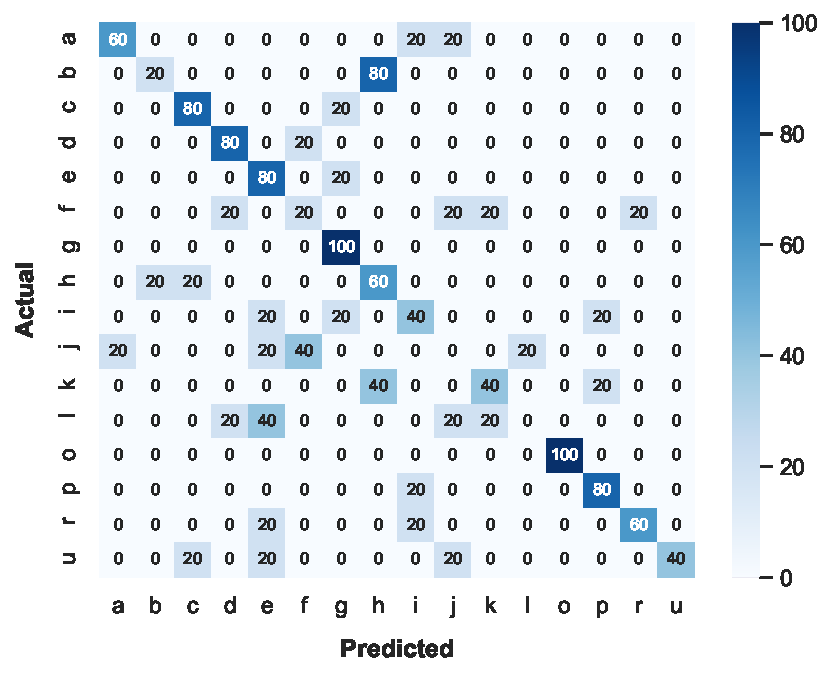
\includegraphics[width=.99\linewidth]{Figures/RadarExperiments/Datasets/SensorsComparison/Horn/confusion-inversion.pdf}
        \vspace{-18pt}
        \captionsetup{width=.99\linewidth}
        \caption{Inversion ($N{=}27$).}
        \label{fig:radar-experiments:sensors:horn-confusion:inversion}
    \end{subfigure}
    \begin{subfigure}{.49\textwidth}
        \centering
        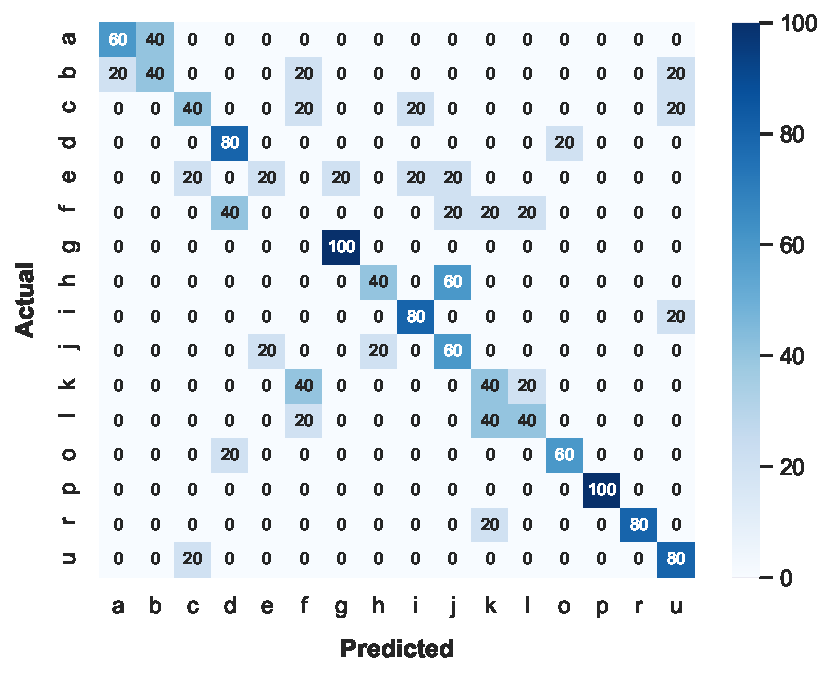
\includegraphics[width=.99\linewidth]{Figures/RadarExperiments/Datasets/SensorsComparison/Horn/confusion-filtering.pdf}
        \vspace{-18pt}
        \captionsetup{width=.99\linewidth}
        \caption{Filtering ($N{=}38$).}
        \label{fig:radar-experiments:sensors:horn-confusion:filtering}
    \end{subfigure}
    
    \vspace{-6pt}
    \caption{Normalized confusion matrices for the best configuration with data acquired from the Horn at four different stages of the pipeline. The values in each cell are represented as percentages.}
    \label{fig:radar-experiments:sensors:horn-confusion}
\end{figure}

% Full-wave inversion
% 53.8\%, 0.5ms ($N{=}27$)
\paragraph{Full-wave inversion.}
The recognition rate decreased significantly after the inversion stage, and reached a maximum of 53.8\% for $N{=}27$ (\fig~\ref{fig:radar-experiments:sensors:horn-samples:inversion}). Average execution time was very short at 0.5 ms. Such a drop was expected, as the size of each frame was divided by 89 compared to the background scene removal stage. 
%
We observed that the recognition rate did not steadily increase with the number of sampling points and could change by more than 10\% between two consecutive values of $N$. This behavior may have been caused by errors in the inversion process, where the distance and apparent permittivity values corresponding to one frame were incorrectly estimated due to the low quality of the radar data (\eg if the received signal was barely above noise level). The filtering stage should help alleviate this problem.
%
\fig~\ref{fig:radar-experiments:sensors:horn-confusion:inversion} shows an average accuracy equal to or higher than 80\% for only six gestures: ``open, then close hand'',  ``extend one/two/four finger(s)'', and ``push fist/palm'' (c, d, e, g, o, p). 
The high accuracy for some of these gestures can be explained by the nature of the permittivity and distance metrics. 
%
The estimated permittivity increases when the hand opens (larger radar cross-section) and decreases when it closes (smaller radar cross-section), which helped distinguish between gestures c, d, e, and g, as they mostly differed in their hand pose.
%
Gestures o and p (push fist/palm) were easy to differentiate from other gestures using the distance metric and the permittivity measure allowed to distinguish between the two.
%
As in the previous stages, the ``swipe'' and ``draw infinity'' gestures (h, i, j, k, l) were more difficult to recognize due to our reliance on data from a single radar antenna.

% Filtering
% 57.5\%, 0.4ms ($N{=}38$)
\paragraph{Filtering.}
As expected, the recognition rate was more stable with respect to the number of sampling points after filtering. However, the best configuration still only reached 57.5\% accuracy for $N{=}30$ (\fig~\ref{fig:radar-experiments:sensors:horn-samples:filtering}), far too low for accurate gesture recognition. 
Execution time was still very short at 0.4 ms. 
The confusion matrix for this configuration (\fig~\ref{fig:radar-experiments:sensors:horn-confusion:filtering}) shows that the recognition rate exceeded 80\% for only six gestures: ``extend one/four fingers'', ``swipe left'', ``push palm'', ``wave hand'', and ``barrier gesture'' (d, g, i, p, r, u). 
%
Some gestures were recognized less accurately after filtering, including ``push fist'' (gesture o), which the recognizer sometimes even failed to match with any other gesture. This could indicate that we applied too much filtering, thus erasing some relevant information from the signal in the process.






\subsubsection{Walabot} \label{sec:radar-experiments:sensors:results:walabot}


% Raw data
\paragraph{Raw data capture.}
% First study - Best antenna pairs
% 88.8\%, 3.6ms ($\splitatcommas{AP{=}(4, 5, 7, 11)}$)
% 86.3\%, 2.8ms ($\splitatcommas{AP{=}(4, 7, 11)}$)
% 86.3\%, 10.5ms ($\splitatcommas{AP{=}(1, 2, 3, 4, 5, 6, 7, 8, 9, 10, 11, 12)}$)
The recognition rate differed widely depending on the set of antenna pairs used for gesture recognition, with larger sets usually achieving better accuracy (\tab~\ref{tab:radar-experiments:sensors:walabot}). 

In the third study, the three best configurations all achieved ${>}86\%$ accuracy on the raw Walabot data: 88.8\% with $\splitatcommas{AP{=}(4, 5, 7, 11)}$, 86.3\% with $\splitatcommas{AP{=}(4, 7, 11)}$, and 86.3\% with $\splitatcommas{AP{=}(1,2,3,4,5,6,7,8,9,10,11,12)}$. Execution time increased with the number of antenna pairs and reached up to 10.5 ms with the set of all antenna pairs. 

\begin{figure}[!t]
    \begin{subfigure}{.49\textwidth}
        \centering
        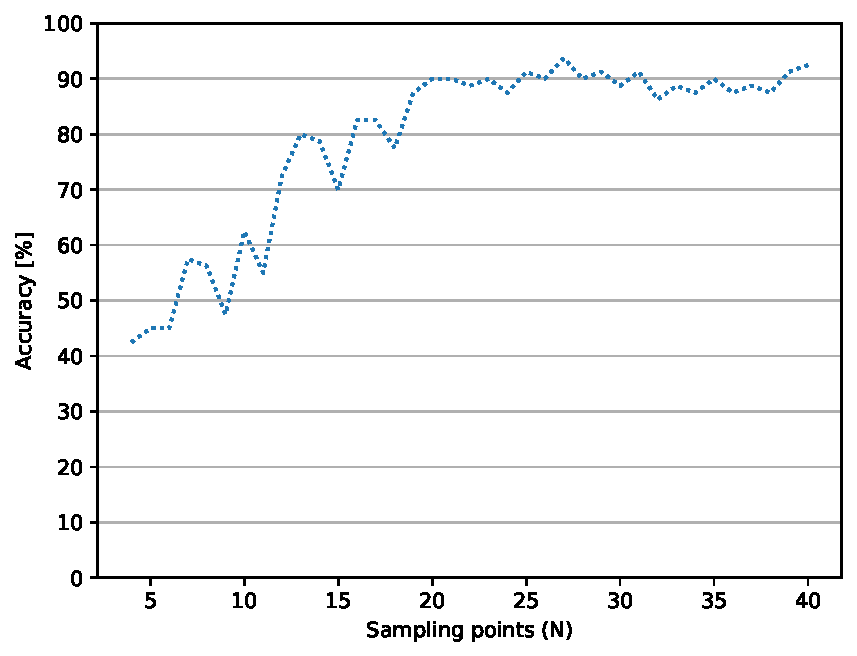
\includegraphics[width=.99\linewidth]{Figures/RadarExperiments/Datasets/SensorsComparison/Walabot/samples-raw.pdf}
        \vspace{-18pt}
        \captionsetup{width=.99\linewidth}
        \caption{Raw data capture \\ $\splitatcommas{AP{=}(1,2,3,6,8,9)}$.}
        \label{fig:radar-experiments:sensors:walabot-samples:raw}
    \end{subfigure}
    \begin{subfigure}{.49\textwidth}
        \centering
        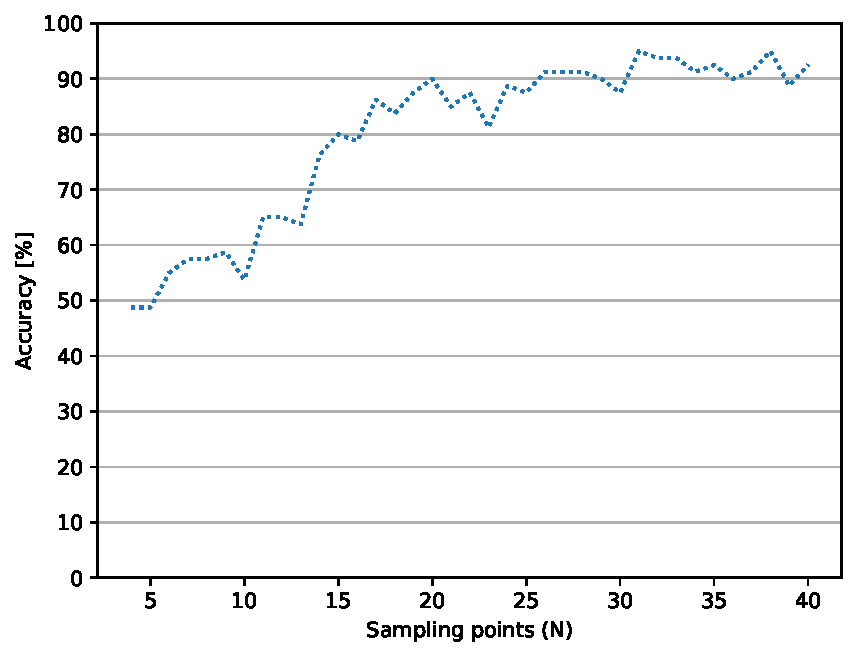
\includegraphics[width=.99\linewidth]{Figures/RadarExperiments/Datasets/SensorsComparison/Walabot/samples-bgsub.pdf}  
        \vspace{-18pt}
        \captionsetup{width=.99\linewidth}
        \caption{Background scene removal \\ $\splitatcommas{AP{=}(4,5,7,10,11,12)}$.}
        \label{fig:radar-experiments:sensors:walabot-samples:bgsub}
    \end{subfigure}
    
    \begin{subfigure}{.49\textwidth}
        \centering
        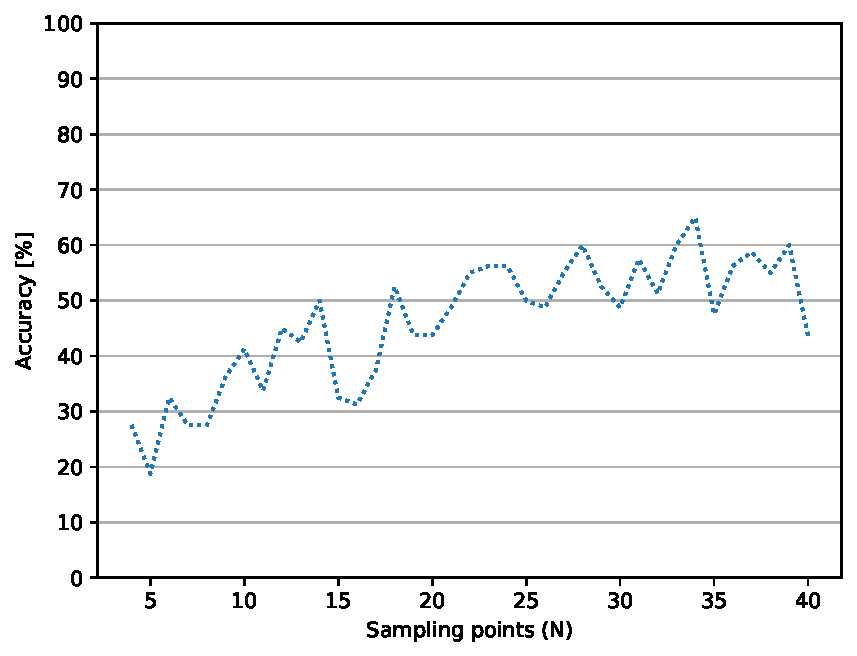
\includegraphics[width=.99\linewidth]{Figures/RadarExperiments/Datasets/SensorsComparison/Walabot/samples-inversion.pdf}
        \vspace{-18pt}
        \captionsetup{width=.99\linewidth}
        \caption{Inversion \\ $\splitatcommas{AP{=}(1,2,3,4,5,6,7,8,9,10,11,12)}$.}
        \label{fig:radar-experiments:sensors:walabot-samples:inversion}
    \end{subfigure}
    \begin{subfigure}{.49\textwidth}
        \centering
        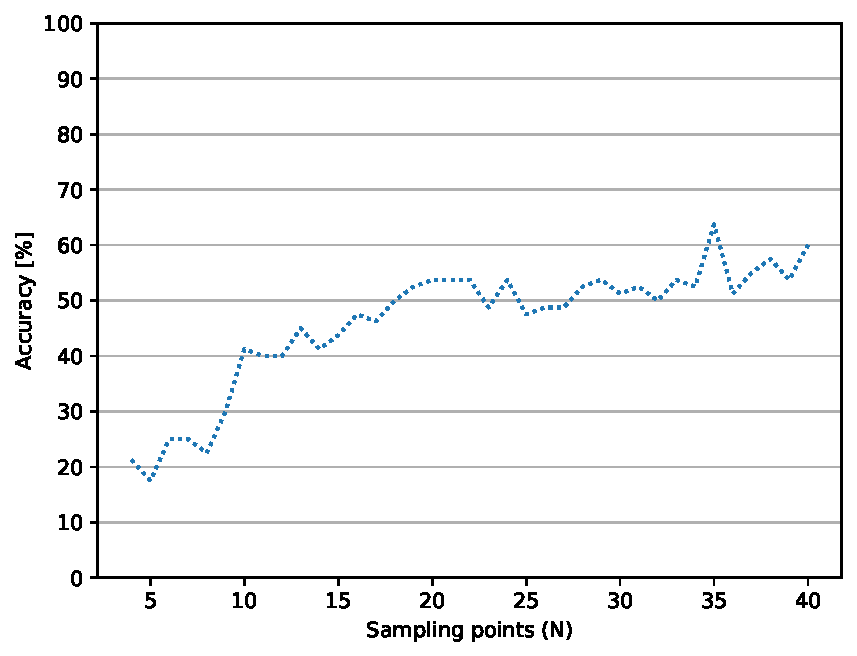
\includegraphics[width=.99\linewidth]{Figures/RadarExperiments/Datasets/SensorsComparison/Walabot/samples-filtering.pdf}
        \vspace{-18pt}
        \captionsetup{width=.99\linewidth}
        \caption{Filtering \\ $\splitatcommas{AP{=}(1,2,3,6,8,9)}$.}
        \label{fig:radar-experiments:sensors:walabot-samples:filtering}
    \end{subfigure}
    
    \vspace{-6pt}
    \caption{The accuracy of Jackknife with respect to the number of sampling points for the best-performing set of antenna pairs with data acquired from the Walabot at four different stages of the pipeline.}
    \label{fig:radar-experiments:sensors:walabot-samples}
\end{figure}


% Second study - Sampling points
% 92.5\%, 5.6ms ($N{=}22$, $\splitatcommas{AP{=}(4, 5, 7, 11)}$)
% 90.0\%, 5.2ms ($N{=}27$, $\splitatcommas{AP{=}(4, 7, 11)}$)
% 93.8\%, 16.7ms ($N{=}23$, $\splitatcommas{AP{=}(1, 2, 3, 4, 5, 6, 7, 8, 9, 10, 11, 12)}$)
% 93.8\%, 10.1ms ($N{=}27$, $\splitatcommas{AP{=}(1, 2, 3, 6, 8, 9)}$)
The three best-performing antenna pairs of the third study were selected for the fourth study and tested along with other sets of antennas. 
%
\fig~\ref{fig:radar-experiments:sensors:walabot-samples:raw} plots the evolution of accuracy with respect to the number of sampling points and for the best-performing set of antenna pairs ($\splitatcommas{AP{=}(1, 2, 3, 6, 8, 9)}$). 
%
Accuracy generally increased with the number of sampling points and reached up to 93.8\% for $N{=}27$, similar to results from the horn session, but slightly higher than the best configuration on the corresponding LMC data. The average execution time for this configuration was 10.1 ms.
%
Other sets of antennas performed worse, with single pairs of antennas achieving between 76.3\% ($N{=}28$, $AP{=}(5)$) and 88.8\% accuracy ($N{=}37$, $AP{=}(9)$).
%
The confusion matrix for the best configuration (\fig~\ref{fig:radar-experiments:sensors:walabot-confusion:raw}) shows that 12 of the 16 gesture classes were correctly recognized 100\% of the time. The remaining gestures were ``close hand'', ``open then close hand'', ``extend two fingers'', and ``swipe down'' (b, c, e, k). Our observations are similar to those we made for the horn data from the LMC+Horn session.
%
In particular, the confusion between gestures e and f (extend three fingers) was likely caused by their similar radar cross-section. 
%
The confusion between gestures k and a (open hand), as well as between gestures b, c, and h (swipe right), is similar to what we observed with the Horn. This suggests that the spacing between Walabot antennas may be too small to accurately distinguish between moving the hand in the plane orthogonal to the radar beam and changing its radar cross-section (\eg fist \vs palm).


% Background scene removal
\paragraph{Background scene removal.}
% Best antenna pairs
% 90.0\%, 3.0ms ($\splitatcommas{AP{=}(4, 7, 11)}$)
% 88.8\%, 3.7ms ($\splitatcommas{AP{=}(4, 7, 11, 12)}$)
% 86.3\%, 3.6ms ($\splitatcommas{AP{=}(4, 5, 7, 11)}$)
Similarly to the Horn, the removal of antenna effects and background subtraction enabled higher recognition rates, with top three configurations achieving ${>}86\%$ accuracy: 90.0\% with $\splitatcommas{AP{=}(4, 7, 11)}$, 88.8\% with $\splitatcommas{AP{=}(4, 7, 11, 12)}$, and 86.3\% with $\splitatcommas{AP{=}(4, 5, 7, 11)}$. Execution time increased with the number of antenna pairs and reached up to 10.6 ms with the set of all antenna pairs. 

% Sampling points
% 91.3\%, 6.1ms ($N{=}28$, $\splitatcommas{AP{=}(4, 7, 11)}$)
% 93.8\%, 7.1ms ($N{=}28$, $\splitatcommas{AP{=}(4, 7, 11, 12)}$)
% 92.5\%, 10.5ms ($N{=}40$, $\splitatcommas{AP{=}(4, 5, 7, 11)}$)
The three best-performing antenna pairs of the third study were selected for the fourth study and tested along with other sets of antennas. 
%
\fig~\ref{fig:radar-experiments:sensors:walabot-samples:bgsub} plots the evolution of accuracy with respect to the number of sampling points and for the best-performing set of antenna pairs ($\splitatcommas{AP{=}(4,5,7,10,11,12)}$). 
%
Accuracy also increased with the number of sampling points, reaching up to 95.0\% for $N{=}31$, which is higher than the raw data and better than the LMC. The average execution time for this configuration was 11.0 ms.
%
The resulting confusion matrix (\fig~\ref{fig:radar-experiments:sensors:walabot-confusion:bgsub}) is extremely similar to the confusion matrix obtained on the raw data. Only four gestures were not correctly recognized 100\% of the time: ``close hand'', ``open then close hand'', ``extend two fingers'', and ``swipe down'' (b, c, e, k).

\begin{figure}[!tb]
    \begin{subfigure}{.49\textwidth}
        \centering
        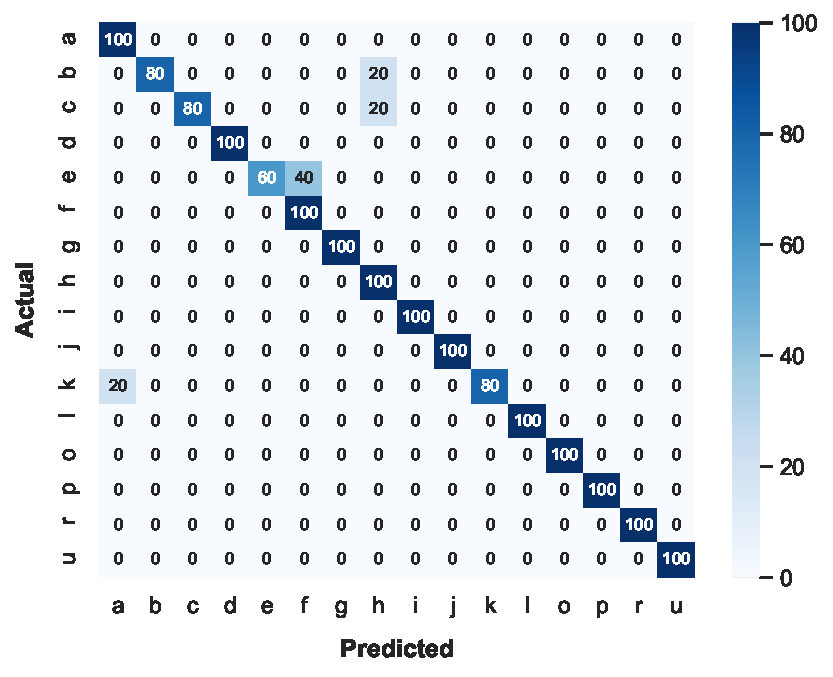
\includegraphics[width=.99\linewidth]{Figures/RadarExperiments/Datasets/SensorsComparison/Walabot/confusion-raw.pdf}
        \vspace{-18pt}
        \captionsetup{width=.95\linewidth}
        \caption{Raw data capture $N{=}27$, \\ $\splitatcommas{AP{=}(1, 2, 3, 6, 8, 9)}$.}
        \label{fig:radar-experiments:sensors:walabot-confusion:raw}
    \end{subfigure}
    \begin{subfigure}{.49\textwidth}
        \centering
        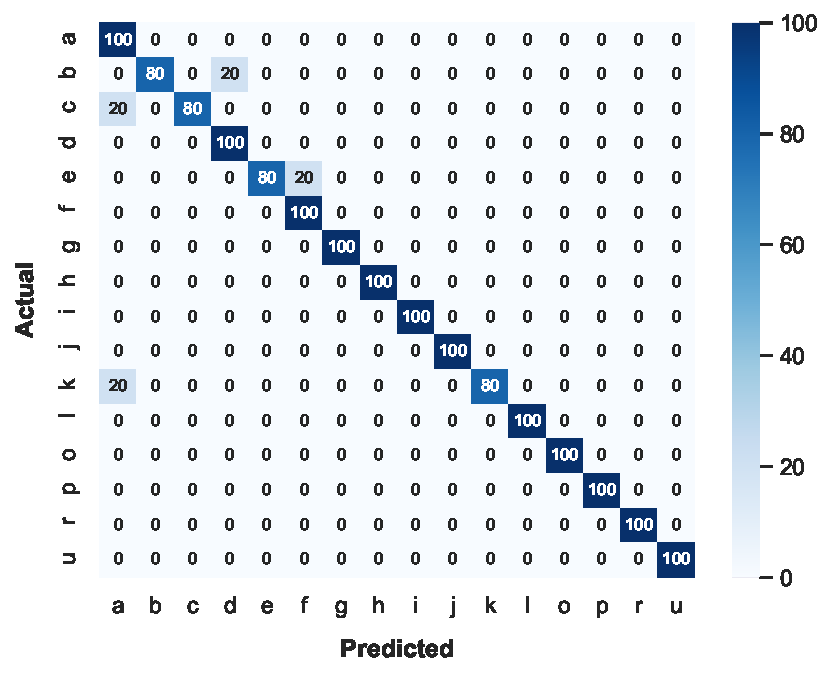
\includegraphics[width=.99\linewidth]{Figures/RadarExperiments/Datasets/SensorsComparison/Walabot/confusion-bgsub.pdf}  
        \vspace{-18pt}
        \captionsetup{width=.95\linewidth}
        \caption{Background scene removal $N{=}31$, \\ $\splitatcommas{AP{=}(4, 5, 7, 10, 11, 12)}$.}
        \label{fig:radar-experiments:sensors:walabot-confusion:bgsub}
    \end{subfigure}
    
    \begin{subfigure}{.49\textwidth}
        \centering
        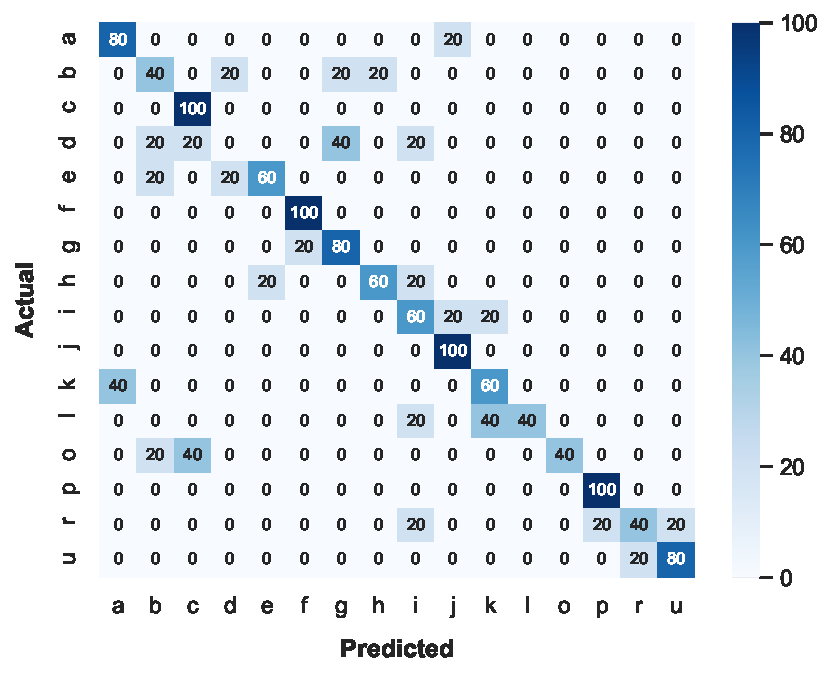
\includegraphics[width=.99\linewidth]{Figures/RadarExperiments/Datasets/SensorsComparison/Walabot/confusion-inversion.pdf}
        \vspace{-18pt}
        \captionsetup{width=.95\linewidth}
        \caption{Inversion $N{=}34$, \\ $\splitatcommas{AP{=}(1,2,3,4,5,6,7,8,9,10,11,12)}$.}
        \label{fig:radar-experiments:sensors:walabot-confusion:inversion}
    \end{subfigure}
    \begin{subfigure}{.49\textwidth}
        \centering
        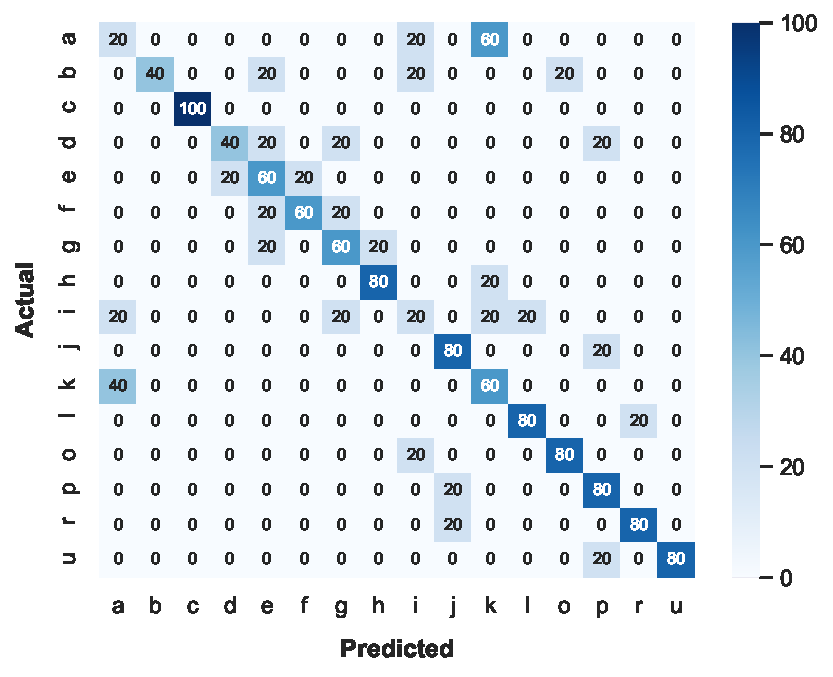
\includegraphics[width=.99\linewidth]{Figures/RadarExperiments/Datasets/SensorsComparison/Walabot/confusion-filtering.pdf}
        \vspace{-18pt}
        \captionsetup{width=.95\linewidth}
        \caption{Filtering $N{=}35$, \\ $\splitatcommas{AP{=}(1, 2, 3, 6, 8, 9)}$.}
        \label{fig:radar-experiments:sensors:walabot-confusion:filtering}
    \end{subfigure}
    
    \vspace{-6pt}
    \caption{Normalized confusion matrices for the best configuration with data acquired from the Walabot at four different stages of the pipeline. The values in each cell are represented as percentages.}
    \label{fig:radar-experiments:sensors:walabot-confusion}
\end{figure}


% Full-wave inversion
\paragraph{Full-wave inversion.}
% Best antenna pairs
% 45.0\%, 0.3ms ($\splitatcommas{AP{=}(4, 7, 10, 11, 12)}$)
% 45.0\%, 0.3ms ($\splitatcommas{AP{=}(2, 3, 8, 9)}$)
% 43.8\%, 0.3ms ($\splitatcommas{AP{=}(1, 2, 3, 6, 8)}$)
The recognition rate for all sets of antenna pairs after the inversion stage was noticeably lower than after the first two stages (\tab~\ref{tab:radar-experiments:sensors:walabot}). Such a drop was expected, as the size of each frame was divided by 34 compared to the first two processing stages. 
%
The best-performing combinations of antenna pairs were: $AP{=}(4, 7, 10, 11, 12)$ with 45.0\% accuracy, $AP{=}(2, 3, 8, 9)$ with 45.0\% accuracy, and $AP{=}(1, 2, 3, 6, 8)$ with 43.8\% accuracy. The average execution time was very short but increased with the number of antenna pairs, reaching up to 0.5 ms with the set of all antenna pairs. 

% Sampling points
% 53.8\%, 0.5ms ($N{=}23$, $\splitatcommas{AP{=}(4, 7, 10, 11, 12)}$)
% 47.5\%, 0.8ms ($N{=}35$, $\splitatcommas{AP{=}(2, 3, 8, 9)}$)
% 53.8\%, 0.9ms ($N{=}38$, $\splitatcommas{AP{=}(1, 2, 3, 6, 8)}$)
As previously, the three best antenna pairs were selected for the fourth study. The accuracy reached 65.0\% with the set of all antenna pairs for $N{=}34$. The execution time was very short, at about 1.3 ms. 
Similar to the Horn, accuracy did not steadily increase with the number of sampling points and could change by nearly 20\% between two consecutive values of $N$. This may be caused by errors in the inversion process and amplified by the lower signal-to-noise ratio of the Walabot.
%
\fig~\ref{fig:radar-experiments:sensors:walabot-confusion:inversion} shows that the recognition rate is higher than 80\% for only seven gestures: ``open hand'', ``open then close hand'', ``extend three/four fingers'', ``swipe up'', ``push palm'', and ``barrier gesture'' (a, c, f, g, j, p, u). 
%
Gestures h, i, j, k, and l (swipe right/left/up/down and draw infinity) were better recognized than with the Horn, indicating that the array of antennas of the Walabot managed to pick up more information to accurately differentiate these similar gestures.

\begin{table}[bt]
    \resizebox{\linewidth}{!}{
    \renewcommand{\arraystretch}{1.1}
    \begin{tabular}{l|rrr|rrr|rrr|rrr}
        \toprule
        & \multicolumn{3}{c|}{\textbf{Raw data}} & \multicolumn{3}{c|}{\textbf{Background subtraction}} & \multicolumn{3}{c|}{\textbf{Full-wave inversion}} & \multicolumn{3}{c}{\textbf{Filtering}}\\
        \cmidrule{2-13}
        \textbf{AP} & \makecell{\textbf{RR} \\{} M (SD) [\%]} & \makecell{\textbf{ET}\\{} [ms]} & \textbf{N} & 
        \makecell{\textbf{RR} \\{} M (SD) [\%]} & \makecell{\textbf{ET}\\{} [ms]} & \textbf{N} & 
        \makecell{\textbf{RR} \\{} M (SD) [\%]} & \makecell{\textbf{ET}\\{} [ms]} & \textbf{N} & 
        \makecell{\textbf{RR} \\{} M (SD) [\%]} & \makecell{\textbf{ET}\\{} [ms]} & \textbf{N} \\
        \midrule
        % Best sets of antenna pairs
        1st best & 92.5 (17.7) & 5.6 & 22 &
        91.3 (14.6) & 6.1 & 28 &
        53.8 (34.0) & 0.5 & 23 &
        56.3 (29.4) & 0.4 & 19 \\

        2nd best & 90.0 (16.3) & 5.2 & 27 &
        93.8 (12.0) & 7.1 & 28 &
        47.5 (27.2) & 0.8 & 35 &
        50.0 (29.2) & 0.3 & 16 \\

        3rd best & \cellcolor{highlightcolor} 93.8 (14.1) & 16.7 & 23 &
        92.5 (12.4) & 10.5 & 40 &
        53.8 (28.0) & 0.9 & 38 &
        60.0 (25.3) & 0.6 & 29 \\

        % Single antenna pairs
        1 & 82.5 (20.5) & 3.4 & 38 &
        77.5 (27.2) & 2.8 & 34 &
        30.0 (23.1) & 0.3 & 22 &
        28.8 (31.0) & 0.0 & 4 \\
        
        2 & 77.5 (20.5) & 3.4 & 37 &
        76.3 (24.5) & 1.7 & 24 &
        18.8 (22.5) & 0.9 & 39 &
        26.3 (30.7) & 0.3 & 36 \\
        
        3 & 81.3 (18.5) & 2.7 & 33 &
        78.8 (21.3) & 2.9 & 39 &
        26.3 (23.9) & 0.9 & 40 &
        30.0 (24.2) & 0.1 & 10 \\
        
        4 & 76.3 (22.2) & 3.1 & 35 &
        81.3 (18.6) & 2.8 & 37 &
        20.0 (14.6) & 0.6 & 35 &
        22.5 (23.0) & 0.1 & 8 \\
        
        5 & 76.3 (18.2) & 2.1 & 28 &
        75.0 (27.8) & 3.1 & 40 &
        21.3 (22.5) & 0.2 & 16 &
        25.0 (29.7) & 0.0 & 4 \\
        
        6 & 81.3 (15.4) & 2.2 & 29 &
        82.5 (19.2) & 2.6 & 32 &
        28.8 (25.3) & 0.7 & 37 &
        31.3 (23.1) & 0.3 & 27 \\
        
        7 & 78.8 (28.7) & 3.1 & 40 &
        80.0 (25.3) & 3.2 & 40 &
        33.8 (26.0) & 0.2 & 16 &
        30.0 (28.3) & 0.2 & 16 \\
        
        8 & 81.3 (20.0) & 2.3 & 26 &
        80.0 (27.3) & 3.1 & 36 &
        27.5 (25.3) & 0.4 & 29 &
        26.3 (28.0) & 0.2 & 17 \\
        
        9 & 88.8 (17.8) & 2.9 & 37 &
        87.5 (16.1) & 2.7 & 31 &
        22.5 (25.2) & 0.0 & 4 &
        30.0 (24.2) & 0.3 & 26 \\
        
        10 & 83.8 (22.2) & 2.6 & 33 &
        80.0 (20.7) & 3.1 & 34 &
        23.8 (22.2) & 0.5 & 28 &
        32.5 (33.4) & 0.0 & 4 \\
        
        11 & 86.3 (21.6) & 3.0 & 37 &
        87.5 (23.0) & 2.9 & 31 &
        23.8 (22.2) & 0.1 & 13 &
        23.8 (20.9) & 0.1 & 7 \\
        
        12 & 77.5 (17.7) & 2.2 & 29 &
        80.0 (19.3) & 2.7 & 31 &
        28.8 (30.1) & 0.5 & 36 &
        31.3 (27.3) & 0.3 & 26 \\
        
        % Largest sets of antenna pairs
        1, 2, 3, 6, 8, 9 & \cellcolor{highlightcolor} 93.8 (12.0) & 10.1 & 27 &
        93.8 (9.6) & 9.6 & 26 &
        61.3 (31.4) & 0.8 & 39 &
        \cellcolor{highlightcolor} 63.8 (23.4) & 0.8 & 35 \\
        
        4, 5, 7, 10, 11, 12 & 92.5 (12.4) & 14.4 & 38 &
        \cellcolor{highlightcolor} 95.0 (8.9) & 11.0 & 31 &
        51.3 (31.0) & 0.6 & 23 &
        56.3 (31.2) & 0.4 & 15 \\
        
        All 12 pairs & \cellcolor{highlightcolor} 93.8 (14.1) & 16.7 & 23 &
        93.8 (12.0) & 28.7 & 38 &
        \cellcolor{highlightcolor} 65.0 (28.8) & 1.3 & 34 &
        58.8 (32.2) & 0.5 & 18 \\
        \bottomrule
    \end{tabular}
    }
    \caption{Recognition rates and execution times obtained for the Walabot data at four steps of the processing pipeline for the first, second, and third best sets of antenna pairs in the third study, all single antenna pairs, the two largest sets of non-redundant antenna pairs, and the set of all antenna pairs. AP=antenna pairs, RR=recognition rate [\%], ET=execution time [ms], N=number of sampling points. The best-performing sets of antenna pairs are highlighted in blue.}
    \label{tab:radar-experiments:sensors:walabot}
    %\vspace{-14pt}
\end{table}

% Filtering
\paragraph{Filtering.}
% Best antenna pairs
% 51.3\%, 0.3ms ($\splitatcommas{AP{=}(1, 2, 6, 8, 9)}$)
% 50.0\%, 0.3ms ($\splitatcommas{AP{=}(1, 2, 8, 9)}$)
% 50.0\%, 0.3ms ($\splitatcommas{AP{=}(4, 7, 10, 11, 12)}$)
The best-performing combinations of antenna pairs after filtering were: 51.3\% with $AP{=}(1, 2, 6, 8, 9)$, 50.0\% with $AP{=}(1, 2, 8, 9)$, and 50.0\% with $AP{=}(4, 7, 10, 11, 12)$.

% Sampling points
% 56.3\%, 0.4ms ($N{=}19$, $\splitatcommas{AP{=}(1, 2, 6, 8, 9)}$)
% 50.0\%, 0.3ms ($N{=}16$, $\splitatcommas{AP{=}(1, 2, 8, 9)}$)
% 60.0\%, 0.6ms ($N{=}29$, $\splitatcommas{AP{=}(4, 7, 10, 11, 12)}$)
The three best antenna pairs were selected for the fourth study. 
The accuracy reached 63.8\% with $AP{=}(1, 2, 3, 6, 8, 9)$ and $N{=}35$. While it is slightly lower than before filtering, the recognition rate was also more stable with respect to the number of sampling points (\fig~\ref{fig:radar-experiments:sensors:walabot-samples:filtering}).
The execution time is still extremely fast at 0.8 ms. 
%
The confusion matrix in \fig~\ref{fig:radar-experiments:sensors:walabot-confusion:filtering} shows that eight gestures were correctly recognized more than 80\% of the time, with only one being correctly recognized 100\% of the time: ``open then close hand'', ``swipe right/up'', ``draw infinity'', ``push fist/palm'', ``wave hand'', and ``barrier gesture'' (c, h, j, l, o, p, r, u).
%
The low signal-to-noise ratio of the Walabot compared to the Horn caused some confusion between gestures d, e, f, g (extend one/two/three/four finger(s)) as they all feature small variations in radar cross-section.
%
Similarly to the previous stage, gestures h, j, k, l, and r (swipe right/up/down, draw infinity, wave hand) were recognized relatively accurately, thanks to the antenna array of the Walabot.
%
However, the spacing between the Walabot antennas is too small to prevent confusion between gesture i (swipe left) and gestures a and b (open/close hand).

%--------------------------------------------------------------------------------%
\subsection{Summary}  \label{sec:radar-experiments:sensors:discussion}
% Summary
Removing the antenna effect and background scene provided minor gains in accuracy compared to relying on the raw radar data. We could see more meaningful gains when using the data from different radars for training and testing.
%
Conversely, the average accuracy dropped after the full-wave inversion stage, reaching a maximum of 65\%, too low for use in actual gesture-based interfaces. 
%
The best performance was achieved with the set of all antenna pairs ($\splitatcommas{AP{=}(1, 2, 3, 4, 5, 6, 7, 8, 9, 10, 11, 12)}$) and the two largest sets of non-redundant antenna pairs ($\splitatcommas{AP{=}(1, 2, 3, 6, 8, 9)}$ and $\splitatcommas{AP{=}(4, 5, 7, 10, 11, 12)}$). The next experiments will thus not evaluate other sets of antenna pairs.
% LMC vs. Walabot vs. Horn
Overall, the Walabot achieved better accuracy than the LMC and the Horn, indicating that inexpensive radars could be used successfully for gesture interaction, at least in a controlled environment. 
% Antennas
The twelve antenna pairs of the Walabot gave it an edge on the Horn's single antenna, despite their lower quality. However, more spaced-out antennas could achieve even better angular resolution, which would benefit some types of gestures, such as ``swipe right/left/up/down'', ``wave hand'', and ``draw infinity''.
%
Using three or more spread-out antennas could also enable us to use trilateration to identify the 3D position of the hand based on data from the full-wave inversion and filtering stages. This could improve the recognition of 3D hand trajectories and be used to display a cursor indicating the position of the user's hand in an application.
%
Finally, sensor fusion techniques such as Kalman filters (Section~\ref{sec:state_of_the_art:overview:challenges:sensors-limitations}) could be leveraged to combine the strengths of radar and vision-based sensors, thus improving gesture recognition accuracy and robustness in challenging environmental conditions.



%================================================================================%
\section{Experiment 2: Gestures Subsets} \label{sec:radar-experiments:gesture-subsets}
%--------------------------------------------------------------------------------%
\subsection{Aims} \label{sec:radar-experiments:gesture-subsets:aims}
This second experiment evaluates the performance of the Walabot on the ``20-gestures'' dataset, a set of 20 hand gestures produced by six participants (Section~\ref{sec:radar-experiments:data-collection:datasets:20-gestures}). It has two main goals:
\begin{enumerate}
    \item Evaluate the efficacy of our signal-processing pipeline on a large set of gestures from multiple users in user-dependent, user-independent, and mixed scenarios.
    \item Explore how smaller, highly differentiable subsets of the gesture set affect the performance of our approach in a user-dependent scenario.
\end{enumerate}

%--------------------------------------------------------------------------------%
\subsection{Protocol} \label{sec:radar-experiments:gesture-subsets:protocol}
This experiment was divided into two studies, both following a similar protocol to the first experiment (Section~\ref{sec:radar-experiments:sensors:protocol}). The \ql testing tool ran on the same computer and used the Jackknife recognizer with the same default settings. The performance of Jackknife was evaluated following a leave-one-out cross-validation (LOOCV) procedure in three user scenarios (see \tab~\ref{tab:quantumleap-testing:testing-procedures} for a detailed description). 
Both studies used the same format for gesture templates as the Walabot studies in the first experiment (Section~\ref{sec:radar-experiments:sensors:protocol:walabot}).
% Each gesture template consists of a sequence of frames, where each frame contains two elements: (1) a timestamp and (2) a vector containing the radar data at that instant. In the inversion and filtering stages, the vector contains two elements: the distance and apparent permittivity evaluated at that instant. In the other stages, the vector (length $2 \times 89$) contains the real and imaginary parts of the frequency-domain radar signal (89 frequencies). 

% All gestures to identify best gesture subsets
\subsubsection{All Gestures} \label{sec:radar-experiments:gesture-subsets:protocol:all-gestures}
The first study of this experiment evaluates the accuracy of Jackknife on the whole dataset at two stages of the radar data processing pipeline in three user scenarios. The study is within-factors with four independent variables:
\begin{enumerate}
    \item \custominlinehighlight{Processing Stage}: nominal variable with two conditions, representing the processing stage of the training data: time gating, filtering.
    \item \custominlinehighlight{User Scenario}: nominal variable with three conditions, representing the type of user scenario: user-dependent, user-independent, mixed.
    \item \custominlinehighlight{Number of Sampling Points}: numerical variable with 37 values representing the number of points per gesture template: $N{=}\{x\in\mathbb{N} \mid 4 \leq x \leq 40\}$.
    \item \custominlinehighlight{Antenna Pairs}: nominal variable with three conditions, representing the selected combination of antenna pairs: $\splitatcommas{AP=\{(1, 2, 3, 6, 8, 9), (4, 5, 7, 10, 11, 12), (1, 2, 3, 4, 5, 6, 7, 8, 9, 10, 11, 12)\}}$.
\end{enumerate}
The total number of training templates per trial is 199 (nine to ten per gesture class) in the user-dependent scenario, 1000 (50 per gesture class) in the user-independent scenario, and 1199 (59 to 60 per gesture class) in the mixed scenario.

\subsubsection{Gesture Subsets} \label{sec:radar-experiments:gesture-subsets:protocol:gesture-subsets}
This second study evaluates the accuracy of Jackknife on subsets of our ``20-gestures'' dataset at two stages of the radar data processing pipeline in a user-dependent scenario. Three of those subsets were created based on our taxonomy (\fig~\ref{fig:radar-experiments:taxonomy}): hand-level, arm-level, and body-level gestures. The other subsets, consisting of highly differentiable gesture classes, were created as follows: (1) identify all subsets with zero (resp. one) confusion between pairs of gesture classes in the results from the previous user-dependent testing, (2) order them by number of gesture classes and total number of confusions, (3) select the largest subset(s) with zero (resp. one) confusion between pairs of gesture classes. We thus have both larger subsets with low confusion between gesture classes and smaller subsets with little to no confusion.  The study is within-factors with four independent variables:
\begin{enumerate}
    \item \custominlinehighlight{Processing Stage}: same as the first study.
    \item \custominlinehighlight{Number of Sampling Points}: same as the first study.
    \item \custominlinehighlight{Antenna Pairs}: same as the first study.
    \item \custominlinehighlight{Gesture Subset}: nominal variable with nine conditions, representing the gesture subset used for training and testing (see \tab~\ref{tab:radar-experiments:subsets}).
\end{enumerate}
The selected subsets are summarized in \tab~\ref{tab:radar-experiments:subsets} and highlighted in \fig~\ref{fig:radar-experiments:confusion-exp1-UD}. 
The time-gating subsets (S6 to S9) consist mostly of arm-level gesture classes, with only two hand-level gesture classes per subset. This indicates that the larger motion of arm-level gestures was easier to differentiate than the smaller-scale hand-level gestures. The filtering subsets (S4 and S5) contain fewer gesture classes than the time-gating subsets, which reflects the high confusion between gesture classes when using data from the filtering stage.
The total number of training templates per trial varies based on the size of the gesture subset but the training sets always feature nine or ten templates per gesture class.

\begin{table}
    \centering
    \footnotesize
    \definecolor{bodylevelcolor}{RGB}{68,84,106}
    \definecolor{armlevelcolor}{RGB}{132,151,176}
    \definecolor{handlevelcolor}{RGB}{214,220,229}
    \begin{tabular}{l|l|l}
        \toprule
        Id & Description & Gestures \\
        \midrule
        S1 & Hand-level & {\circled[black]{a}{handlevelcolor}\circled[black]{b}{handlevelcolor}\circled[black]{c}{handlevelcolor}\circled[black]{d}{handlevelcolor}\circled[black]{e}{handlevelcolor}\circled[black]{f}{handlevelcolor}\circled[black]{g}{handlevelcolor}}\\
        S2  & Arm-level & \circled{h}{armlevelcolor}\circled{i}{armlevelcolor}\circled{j}{armlevelcolor}\circled{k}{armlevelcolor}\circled{l}{armlevelcolor}\circled{m}{armlevelcolor}\circled{n}{armlevelcolor}\circled{o}{armlevelcolor}\circled{p}{armlevelcolor}\circled{r}{armlevelcolor}\circled{s}{armlevelcolor}\\
        S3  & Body-level & \circled{u}{bodylevelcolor}\circled{v}{bodylevelcolor}\\
        \midrule
        S4 & Filtering, C=0 & \circled[black]{b}{handlevelcolor}\circled[black]{g}{handlevelcolor}\circled{l}{armlevelcolor}\\ % 2, 11, 16
        S5 & Filtering, C=1 & \circled[black]{b}{handlevelcolor}\circled[black]{g}{handlevelcolor}\circled{h}{armlevelcolor}\circled{l}{armlevelcolor}\\ % 2, 4, 11, 16
        S6 & Time gating, C=0 (a) & \circled[black]{a}{handlevelcolor}\circled[black]{e}{handlevelcolor}\circled{h}{armlevelcolor}\circled{k}{armlevelcolor}\circled{m}{armlevelcolor}\circled{n}{armlevelcolor}\circled{o}{armlevelcolor}\circled{r}{armlevelcolor}\\ % 1, 4, 7, 8, 10, 14, 18, 19
        S7 & Time gating, C=0 (b) & \circled[black]{a}{handlevelcolor}\circled[black]{e}{handlevelcolor}\circled{h}{armlevelcolor}\circled{k}{armlevelcolor}\circled{n}{armlevelcolor}\circled{o}{armlevelcolor}\circled{r}{armlevelcolor}\circled{v}{bodylevelcolor}\\ % 1, 4, 7, 8, 10, 14, 19, 20
        S8 & Time gating, C=1 (a) & \circled[black]{b}{handlevelcolor}\circled[black]{f}{handlevelcolor}\circled{h}{armlevelcolor}\circled{i}{armlevelcolor}\circled{j}{armlevelcolor}\circled{l}{armlevelcolor}\circled{m}{armlevelcolor}\circled{n}{armlevelcolor}\circled{p}{armlevelcolor}\circled{r}{armlevelcolor}\circled{s}{armlevelcolor}\circled{v}{bodylevelcolor}\\ % 2, 4, 5, 6, 9, 10, 11, 15, 17, 18, 19, 20
        S9 & Time gating, C=1 (b) & \circled[black]{b}{handlevelcolor}\circled[black]{f}{handlevelcolor}\circled{h}{armlevelcolor}\circled{i}{armlevelcolor}\circled{k}{armlevelcolor}\circled{l}{armlevelcolor}\circled{m}{armlevelcolor}\circled{n}{armlevelcolor}\circled{p}{armlevelcolor}\circled{r}{armlevelcolor}\circled{s}{armlevelcolor}\circled{v}{bodylevelcolor}\\ % 2, 4, 5, 7, 9, 10, 11, 15, 17, 18, 19, 20
        \bottomrule
    \end{tabular}
    \caption{The nine selected subsets of gestures. C represents the maximum number of confusion between pairs of gestures. Gestures are colored based on the taxonomy in \fig~\ref{fig:radar-experiments:taxonomy}.}
    \label{tab:radar-experiments:subsets}
    % \vspace{-14pt}
\end{table}

%--------------------------------------------------------------------------------%
\subsection{Results} \label{sec:radar-experiments:gesture-subsets:results}

\subsubsection{All Gestures} \label{sec:radar-experiments:gesture-subsets:results:all-gestures}
% User-dependent
Accuracy reaches 90.6\% over the whole dataset in the user-dependent scenario using data from the time gating stage, with an average execution time of 34ms ($N{=}38$, $\splitatcommas{AP{=}(4, 5, 7, 10, 11, 12)}$). 
We observe more confusion between gesture classes d, e, f, g, and p (extend one/two/three/four finger(s), push palm), most of which fall under 90\% accuracy. These gestures feature small changes in hand pose (and thus, slight variations in the amplitude of the reflected signal) and similar trajectories, making them tricky to differentiate. Some confusion is also observed between gestures j and k (swipe up and down), whose opposite trajectories result in very similar radar signatures. Conversely, seven gesture classes reach over 95\% accuracy, including one hand-level gesture (j - swipe up), five arm-level gestures (h, i, l, m, and n - swipe right/left, draw infinity/circle/Z), and one body-level gesture (v - barrier gesture). 
% Gesture class l is even recognized correctly 100\% of the time.
%
Accuracy drops to 45.2\% with data from the filtering stage ($N{=}26$, $\splitatcommas{AP{=}(1, 2, 3, 4, 5, 6, 7, 8, 9, 10, 11, 12)}$), with a much shorter execution time at 2ms.
Only seven gesture classes are recognized with more than 50\% accuracy, namely b, k, l, m, n, p, and s (close hand, swipe down, draw infinity/circle/Z, push palm, knock twice). All but two of these classes (b and s) feature different motions in space with similar hand poses. The distance measurement is thus crucial for distinguishing between these gesture classes, while the relative permittivity is less relevant.
%such, the distance measure should be These gestures differ in their trajectory, rather than their hand pose, and should thus rely more on the distance measurement than the permittivity measure.
We also observe some confusion between gesture classes d, e, f, g, o, and p (extend one/two/three/four finger(s), push fist/palm), which feature different hand poses but similar trajectories. In particular, gestures d and o are recognized with less than 30\% accuracy. The relative permittivity is more relevant than the distance measure to identify hand poses. As such, the permittivity measures may lack the required precision to accurately distinguish between these slight variations in hand poses, thus explaining the lower accuracy on these gesture classes. In this context, it is noteworthy to mention that the obtained permittivity values exhibit high sensitivity to minor shifts in hand orientation, rendering them susceptible to recognition inaccuracies.
%
\fig~\ref{fig:radar-experiments:confusion-exp1-UD} shows the confusion matrices corresponding to these two configurations. 

% User-independent
Accuracy decreased sharply in the user-independent scenario, dropping to 24.6\% using data from the time gating stage ($N{=}38$, $\splitatcommas{AP{=}(1, 2, 3, 6, 8, 9)}$).
Looking at the performance for each gesture class shows similar patterns to the user-dependent scenario, albeit with much lower accuracy. There was a lot of confusion between gesture classes a, b, c, d, e, f, g, and p (open/close hand, open then close hand, extend one/two/three/four finger(s), push palm). Only five gesture classes reached more than 30\% accuracy, namely k, m, p, u, and v (swipe down, draw circle, push palm, barrier gesture, touch nose). In particular, class k, which had a very different radar signature than most other gestures, was accurately recognized 77\% of the time.
%
Accuracy was only 15.8\% with data from the filtering stage ($N{=}29$, $\splitatcommas{AP{=}(1, 2, 3, 4, 5, 6, 7, 8, 9, 10, 11, 12)}$). Patterns are very hard to distinguish in this scenario because of the very low accuracy. Only two gesture classes reached 30\% accuracy, namely, classes m and n (draw circle/Z). Some form of normalization of the signal with respect to the users could be applied to improve the performance of the system.
%
\fig~\ref{fig:radar-experiments:confusion-exp1-UI} shows the confusion matrices corresponding to these two configurations. 

% Mixed
In the mixed scenario, accuracy was only slightly lower than in the user-dependent scenario, reaching 90.3\% with data from the time gating stage ($N{=}39$, $\splitatcommas{AP{=}(1, 2, 3, 6, 8, 9)}$), and 40.2\% with data from the filtering stage ($N{=}25$, $\splitatcommas{AP{=}(1, 2, 3, 4, 5, 6, 7, 8, 9, 10, 11, 12)}$). Execution time was longer, reaching 203ms (resp. 12ms) with time-domain (resp. inversion) data.
Confusion matrices in this scenario are similar to the user-dependent scenario, with similar observations (\fig~\ref{fig:radar-experiments:confusion-exp1-Mixed}).

\begin{figure}
    \centering
    \begin{subfigure}{.69\linewidth}
        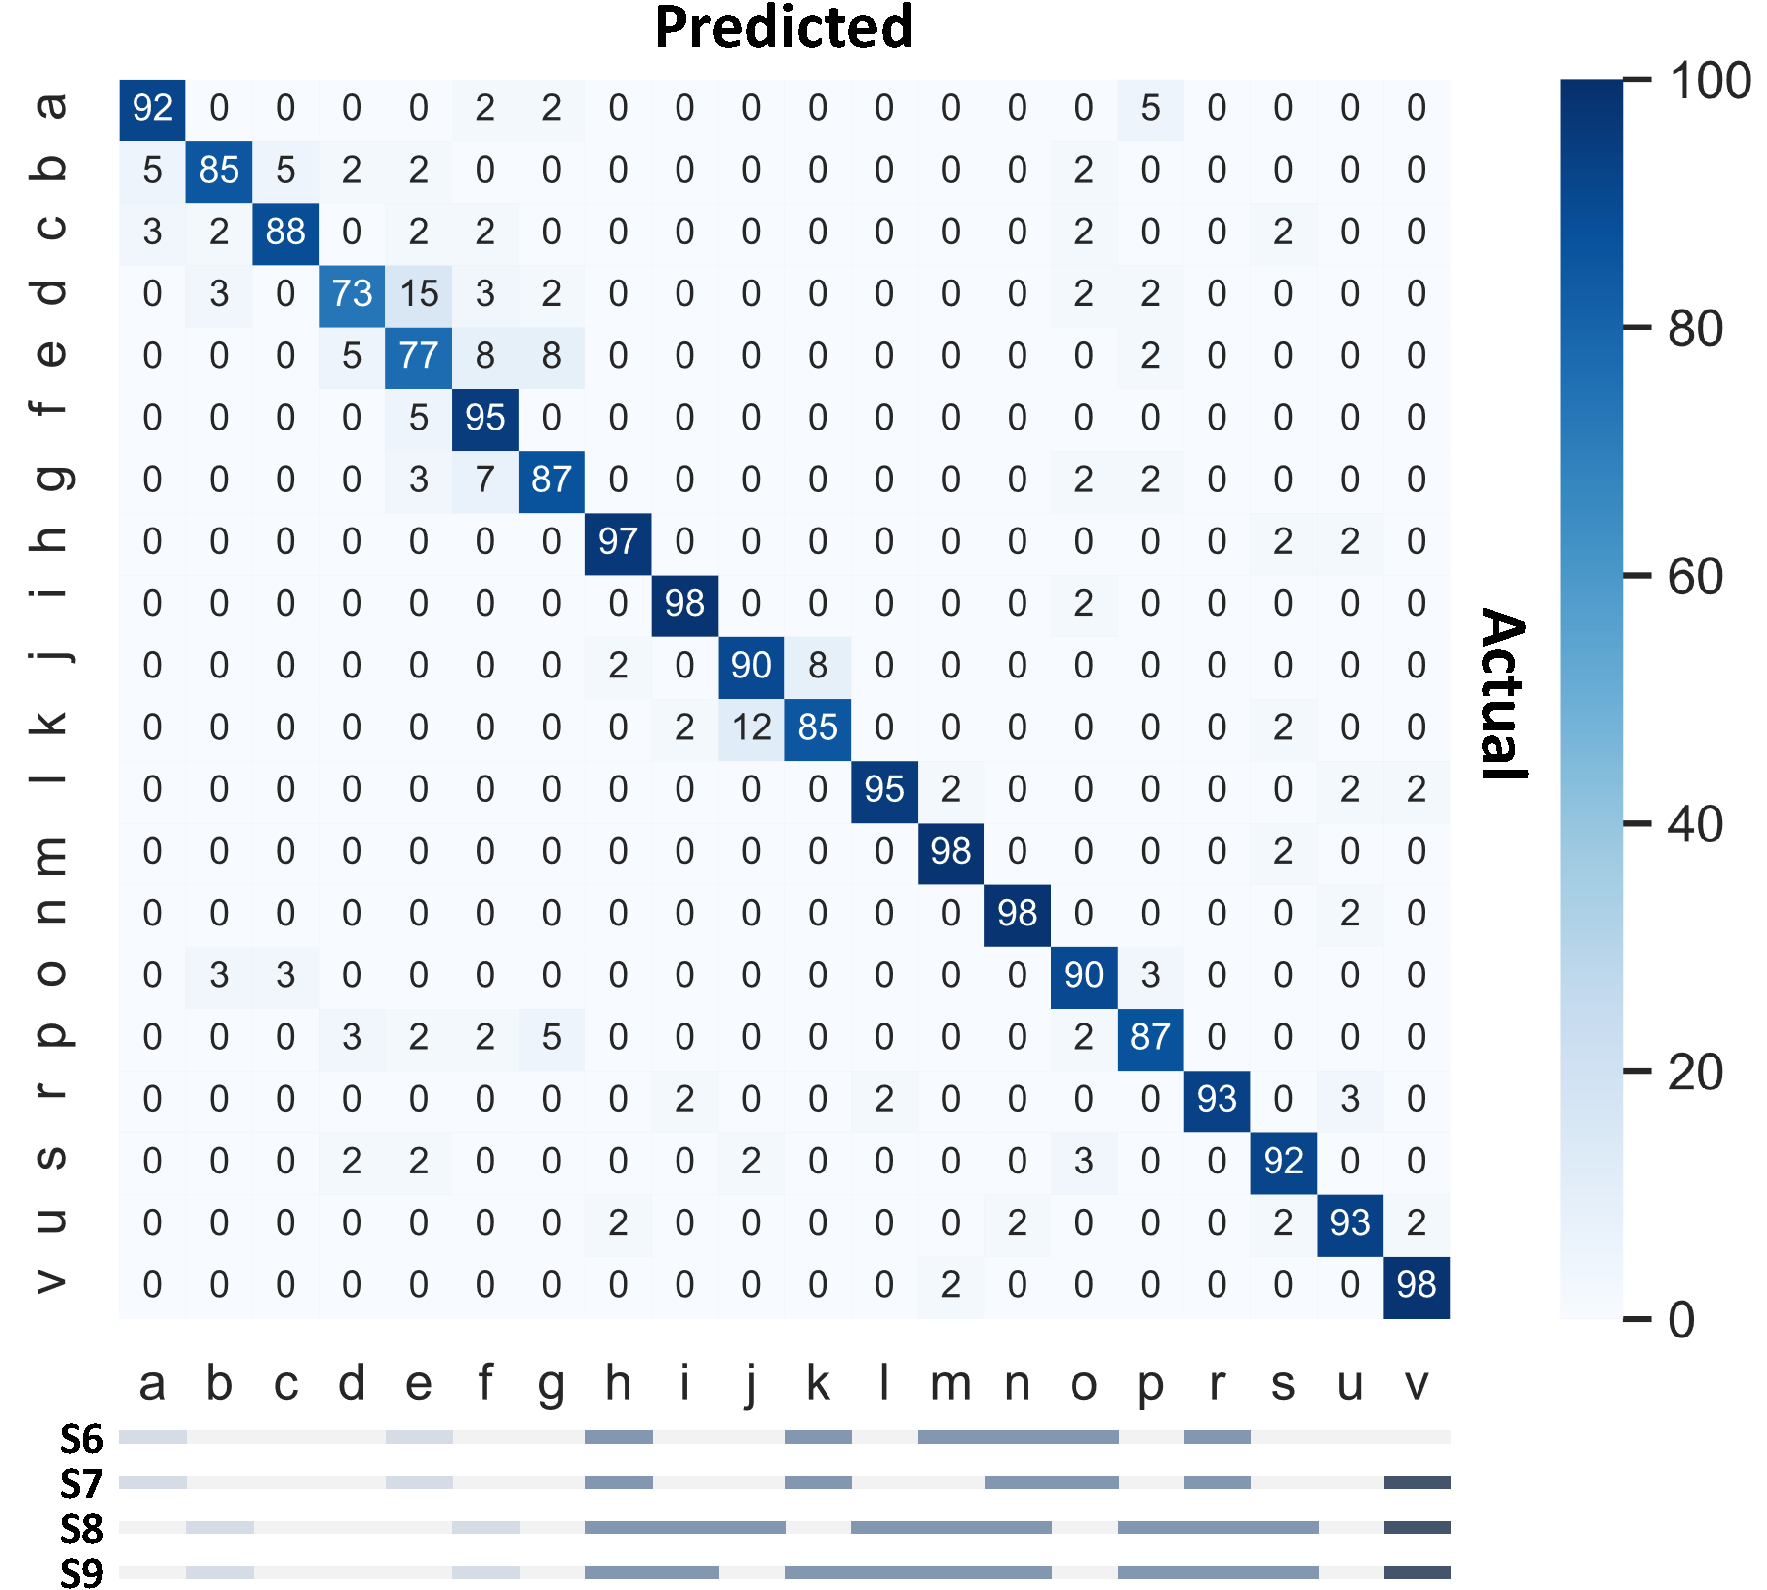
\includegraphics[width=\linewidth]{Figures/RadarExperiments/Datasets/20Gestures/Results/All/UD-time-gating-38-4_5_7_10_11_12-cm-2.pdf}
        \vspace{-12pt}
        \caption{Time gating stage $N{=}38$, \\ $\splitatcommas{AP{=}(4, 5, 7, 10, 11, 12)}$.}
        \vspace{6pt}
        \label{fig:radar-experiments:confusion-exp1-UD-timegating}
    \end{subfigure}
    \begin{subfigure}{.69\linewidth}
        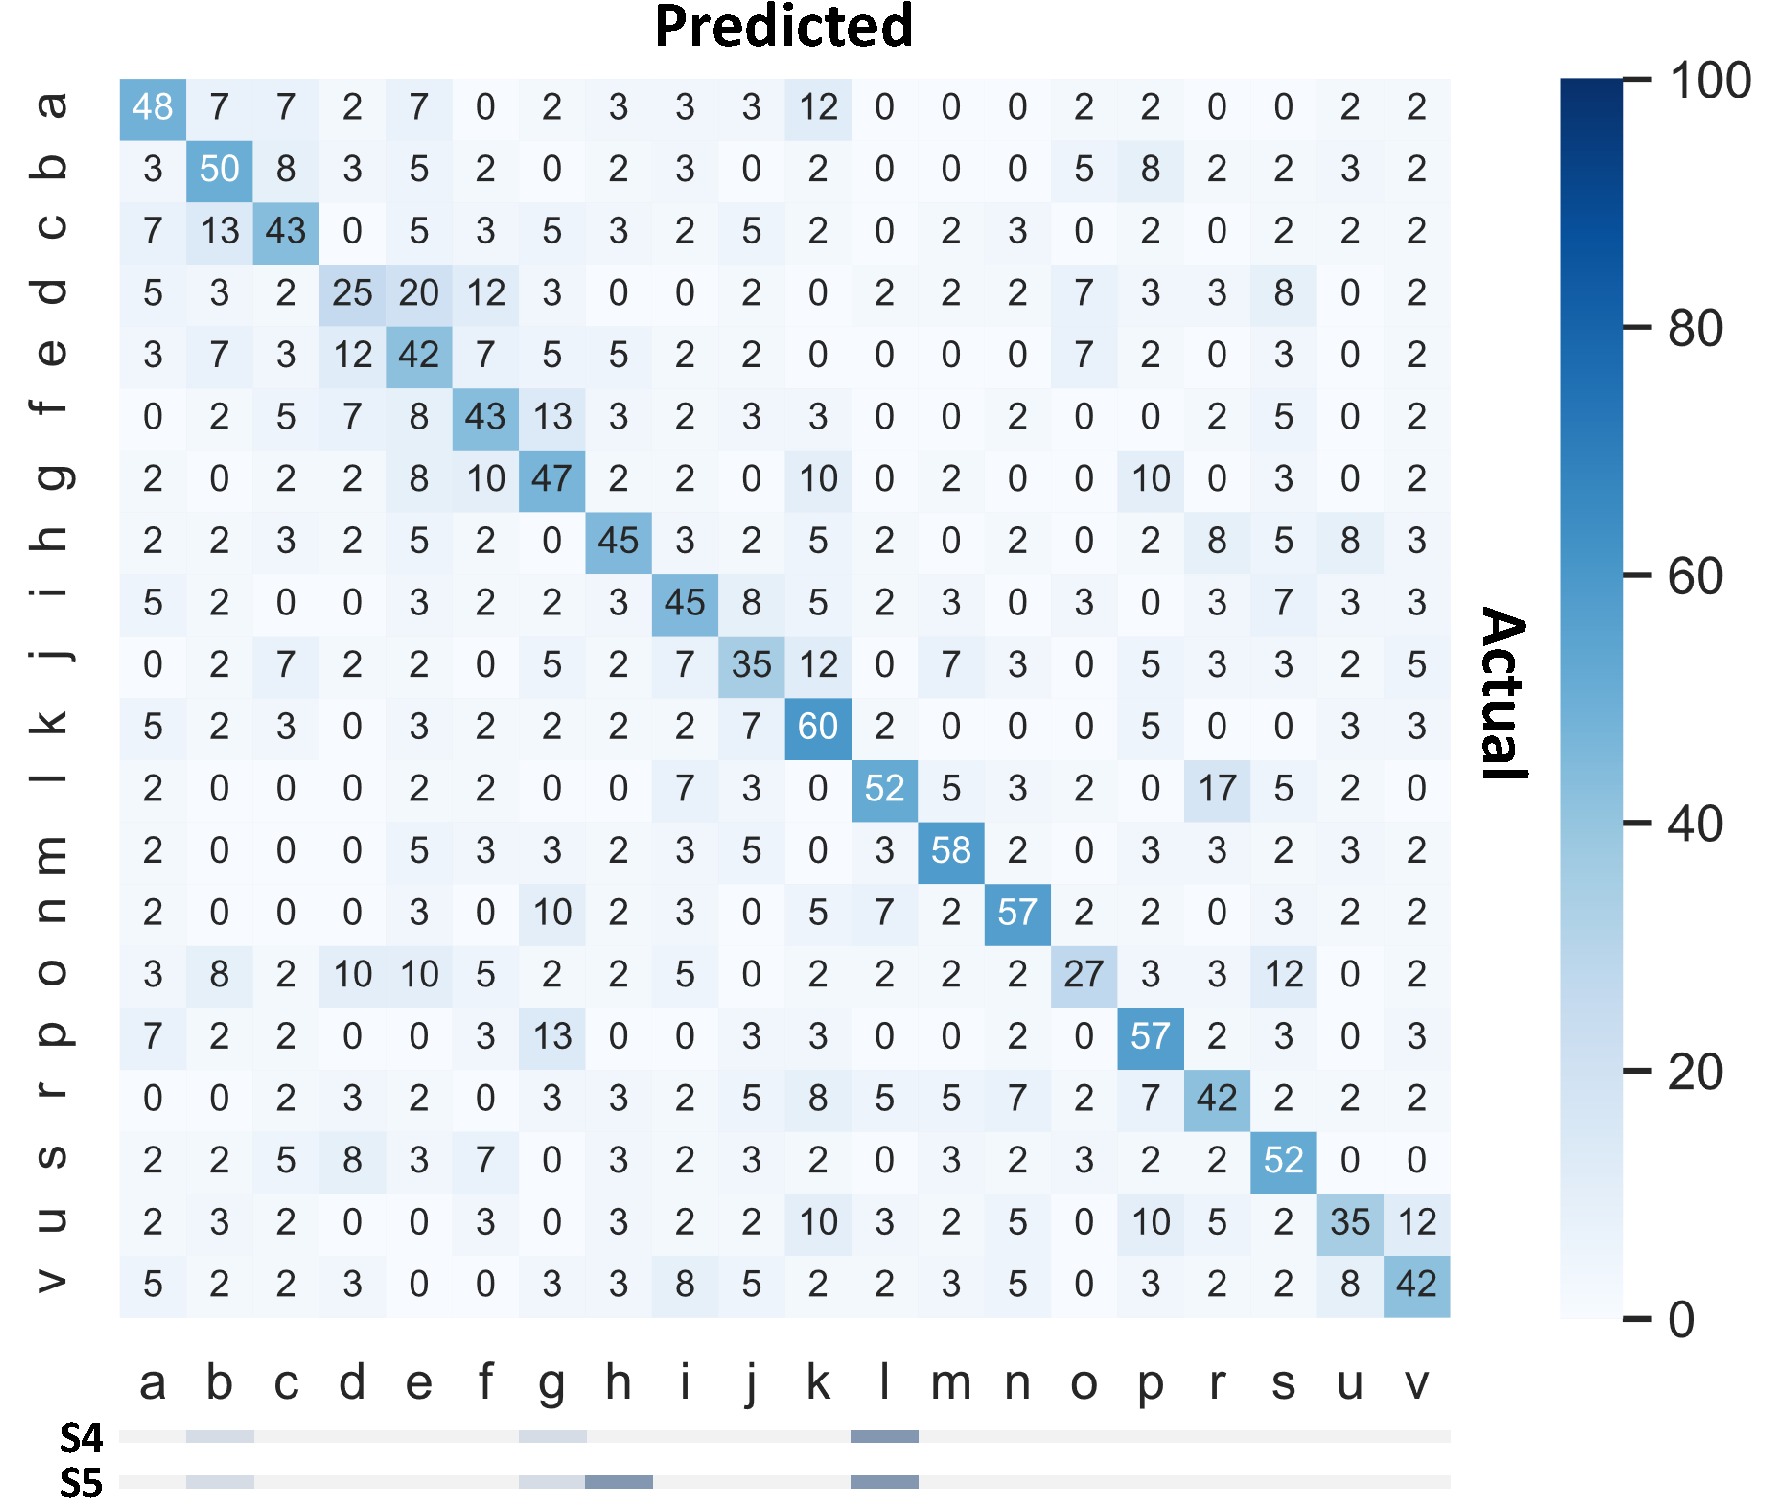
\includegraphics[width=\linewidth]{Figures/RadarExperiments/Datasets/20Gestures/Results/All/UD-Filtering-26-1_2_3_4_5_6_7_8_9_10_11_12-cm-2.pdf}
        \vspace{-12pt}
        \caption{Filtering stage $N{=}26$, \\ $\splitatcommas{AP{=}(1, 2, 3, 4, 5, 6, 7, 8, 9, 10, 11, 12)}$.}
        \label{fig:radar-experiments:confusion-exp1-UD-filtering}
    \end{subfigure}
    \caption{Confusion matrices of the best-performing configurations in the user-dependent scenario on the complete dataset.}
    \label{fig:radar-experiments:confusion-exp1-UD}
    \vspace{-20pt}
\end{figure}

\begin{figure}
    \centering
    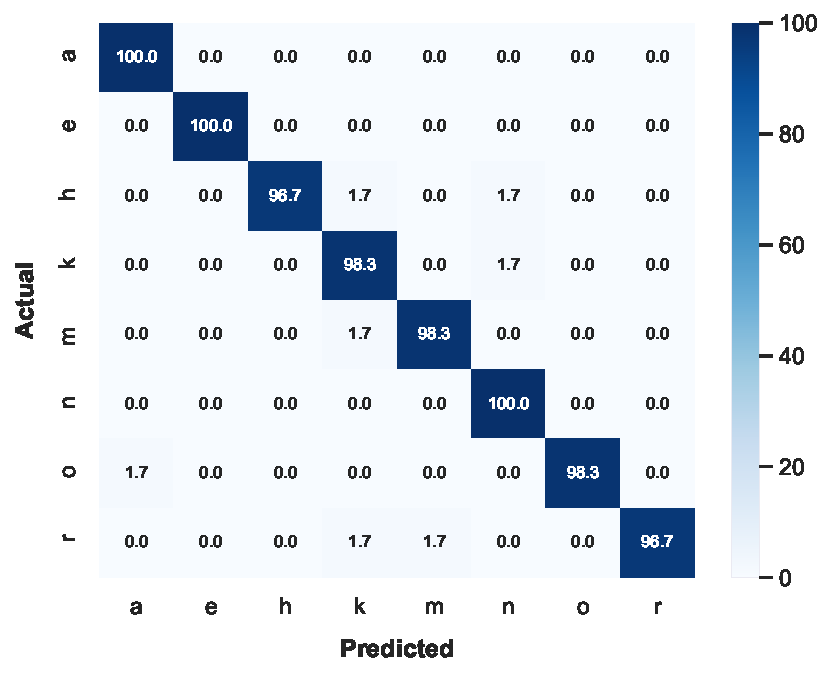
\includegraphics[width=.72\linewidth]{Figures/RadarExperiments/Datasets/20Gestures/Results/1_4_7_8_10_14_18_19/1f-cm.pdf}
    \caption{Confusion matrix of the best-performing configuration on gesture subset S6 (time gating stage).}
    \label{fig:confusion-exp2-S6}
    % \vspace{-12pt}
\end{figure}


\subsubsection{Gesture Subsets} \label{sec:radar-experiments:gesture-subsets:results:gesture-subsets}
% Three subsets based on the taxonomy (S1, S2, S3)
% Time gating
Despite containing fewer gestures, the classification accuracy on subset S1 (hand-level) was lower than on the full set of gestures, at 87.9\% ($N{=}35$, $\splitatcommas{AP{=}(1, 2, 3, 4, 5, 6, 7, 8, 9, 10, 11, 12)}$).
Conversely, the accuracy on the larger S2 subset (arm-level) was higher, at 96.2\% ($N{=}37$, $\splitatcommas{AP{=}(1, 2, 3, 6, 8, 9)}$), indicating that arm-level gestures may be easier to differentiate with our technique than smaller-scale gestures.
Accuracy on body-level gestures (S3) was even higher at 99.2\% ($N{=}20$, $AP{=}(4, 5, 7, 10, 11, 12)$), but the small size of this subset left less room for confusion between gestures.
% Filtering
As expected, classification accuracy was lower on data from the filtering stage, with the accuracy for hand-, arm-, and body-level gestures reaching 51.9\% ($N{=}26$, $\splitatcommas{AP{=}(1, 2, 3, 4, 5, 6, 7, 8, 9, 10, 11, 12)}$), 55.5\% ($N{=}34$, $\splitatcommas{AP{=}(1, 2, 3, 4, 5, 6, 7, 8, 9, 10, 11, 12)}$), and 80.0\% ($N{=}28$, $\splitatcommas{AP{=}(4, 5, 7, 10, 11, 12)}$), respectively. A similar pattern emerged, however, with arm-level gestures being classified more accurately than hand-level ones despite the greater size of the subset.

% Filtering subsets (S4, S5)
The accuracy on subsets S4 and S5 with data from the filtering stage was relatively low considering the size of the subsets: 86.1\% ($N{=}22$, $\splitatcommas{AP{=}(1, 2, 3, 4, 5, 6, 7, 8, 9, 10, 11, 12)}$) and 77.5\% ($N{=}23$, $\splitatcommas{AP{=}(1, 2, 3, 4, 5, 6, 7, 8, 9, 10, 11, 12)}$) for three and four gesture classes, respectively.
% Time gating subsets (S6, S7, S8, S9)
Conversely, Jackknife managed a high accuracy of 98.5\% on subsets S6 ($N{=}38$, $\splitatcommas{AP{=}(4, 5, 7, 10, 11, 12)}$) and S7 ($N{=}38$, $\splitatcommas{AP{=}(4, 5, 7, 10, 11, 12)}$) using data from the time gating stage. Accuracy was still high at 97.8\% and 97.5\% on the larger S8 ($N{=}38$, $\splitatcommas{AP{=}(4, 5, 7, 10, 11, 12)}$) and S9 ($N{=}37$, $\splitatcommas{AP{=}(4, 5, 7, 10, 11, 12)}$) subsets, respectively. Other subsets could perform even better but testing them all would be unrealistic due to the large number of subsets.



%--------------------------------------------------------------------------------%
\subsection{Summary} \label{sec:radar-experiments:gesture-subsets:discussion}
% Discussion
Overall, the best performance on the whole dataset was achieved in user-dependent and mixed scenarios, using data from the time-gating stage of our processing strategy. 
For real-time execution in a mixed scenario, the number of training samples should be carefully selected to maximize accuracy while minimizing the response time of the system, which depends mostly on the execution time of the recognizer. 
The good performance of the system in the mixed scenario showed that it could accurately recognize the gestures of one user, even when the training set featured other users' samples. 
This property makes the combination of our pipeline and the Jackknife recognizer ideal for building gestural interfaces that are trained and used by a small set of users, such as a gesture-based TV remote. 
In addition, the use of a template-matching recognizer enables quick and easy customization of the gesture set.

The evaluation of nine gesture subsets showed that the Walabot had some trouble differentiating between hand gestures that featured small differences in radar cross-section, while arm-level gestures were easier to differentiate.
%
In addition, it suggested that using smaller, well-differentiated sets of gestures could be the key to building reliable radar-based gesture recognition. 
%
Our method for subset selection (Section~\ref{sec:radar-experiments:gesture-subsets:protocol:gesture-subsets}) managed to effectively produce highly-differentiable sets of gestures. Although better subsets may be identified by testing all possible combinations, this becomes unrealistic as the pool of potential gestures grows.


%================================================================================%
\section{Experiment 3: Gestures through Materials} \label{sec:radar-experiments:through-materials}

%--------------------------------------------------------------------------------%
\subsection{Aims} \label{sec:radar-experiments:through-materials:aims}
Radar sensing can penetrate non-conducting materials, such as glass, wood, and plastic, thus making it appropriate for gesture recognition in environments with poor visibility, \eg due to occlusion, which are often incompatible with other types of sensors. This third and last experiment investigates the performance of the Walabot on the ``through-materials'' dataset, a set of nine hand gestures performed by 20 participants sensed through three types of materials (wood, PVC, and glass). It has two main goals:
\begin{enumerate}
    \item Evaluate the performance of the Walabot for sensing gestures through wood, PVC, and glass.
    \item Evaluate the ability of our signal-processing pipeline to normalize radar data collected through different materials.
\end{enumerate}
The experiment described in this section is similar to a study conducted by Leiva \etal~\cite{Leiva:2020}, that analyzed the impact on gesture recognition accuracy of different fabrics covering a Google Soli radar. 

%--------------------------------------------------------------------------------%
\subsection{Protocol} \label{sec:radar-experiments:through-materials:protocol}
This experiment consists of two studies that follow a similar protocol to the first two experiments (Sections~\ref{sec:radar-experiments:sensors:protocol} and~\ref{sec:radar-experiments:gesture-subsets}). The \ql testing tool ran on the same computer and used the Jackknife recognizer with the same default settings. The performance of Jackknife was evaluated following a leave-one-out cross-validation (LOOCV) procedure (see \tab~\ref{tab:quantumleap-testing:testing-procedures} for a detailed description).
The gesture template format was similar to the first two experiments but featured time-domain data instead of frequency-domain data for the background subtraction stage, which should be less sensitive to the number of sampling points and result in better accuracy across different users and materials. 

\subsubsection{Intra-material} \label{sec:radar-experiments:through-materials:protocol:intra-material}
This first study evaluates the accuracy of Jackknife on data recorded through three different materials, at two stages of the radar data processing pipeline and in two user scenarios. Data from the same material is used for training and testing. The study is within-factors with six independent variables:
\begin{enumerate}
    \item \custominlinehighlight{Processing Stage}: nominal variable with two conditions, representing the processing stage of the training data: time gating, filtering.
    \item \custominlinehighlight{User Scenario}: nominal variable with two conditions, representing the type of user scenario: user-dependent, user-independent.
    \item \custominlinehighlight{Material}: nominal variable with three conditions, representing the type of material used for both training and testing: wood, PVC, glass.
    \item \custominlinehighlight{Number of Sampling Points}: numerical variable with 37 values representing the number of points per gesture template: $N{=}\{x\in\mathbb{N} \mid 4 \leq x \leq 40\}$.
    \item \custominlinehighlight{Antenna Pairs}: nominal variable with three conditions, representing the selected combination of antenna pairs: $\splitatcommas{AP=\{(1, 2, 3, 6, 8, 9), (4, 5, 7, 10, 11, 12), (1, 2, 3, 4, 5, 6, 7, 8, 9, 10, 11, 12)\}}$.
\end{enumerate}
% In the rest of this section, we refer to trials using the same (resp. different) training and testing materials as ``intra-material'' (resp. ``inter-materials'').
The total number of training templates per trial is 44 (four to five per gesture class) in the user-dependent scenario and 855 (95 per gesture class) in the user-independent scenario.

\subsubsection{Inter-material} \label{sec:radar-experiments:through-materials:protocol:inter-material}
This second study evaluates the accuracy of Jackknife when tested on data recorded through a different type of material than its training data, at two stages of the radar data processing pipeline in a user-dependent and cross-dataset scenario. The study is within-factors with four independent variables:
{\sloppy
\begin{enumerate}
    \item \custominlinehighlight{Processing Stage}: same as the first study.
    \item \custominlinehighlight{Materials}: nominal variable with six conditions, representing the combination of materials used for training and testing the recognizer (\textit{training}+\textit{testing}): wood+PVC, wood+glass, PVC+wood, PVC+glass, glass+wood, and glass+PVC.
    \item \custominlinehighlight{Number of Sampling Points}: same as the first study.
    \item \custominlinehighlight{Antenna Pairs}: same as the first study.
\end{enumerate}
}
The total number of training templates per trial is 45 (five per gesture class).

%--------------------------------------------------------------------------------%
\subsection{Results} \label{sec:radar-experiments:through-materials:results}

\begin{figure}[hbtp]
    \centering
    \begin{subfigure}{\linewidth}
        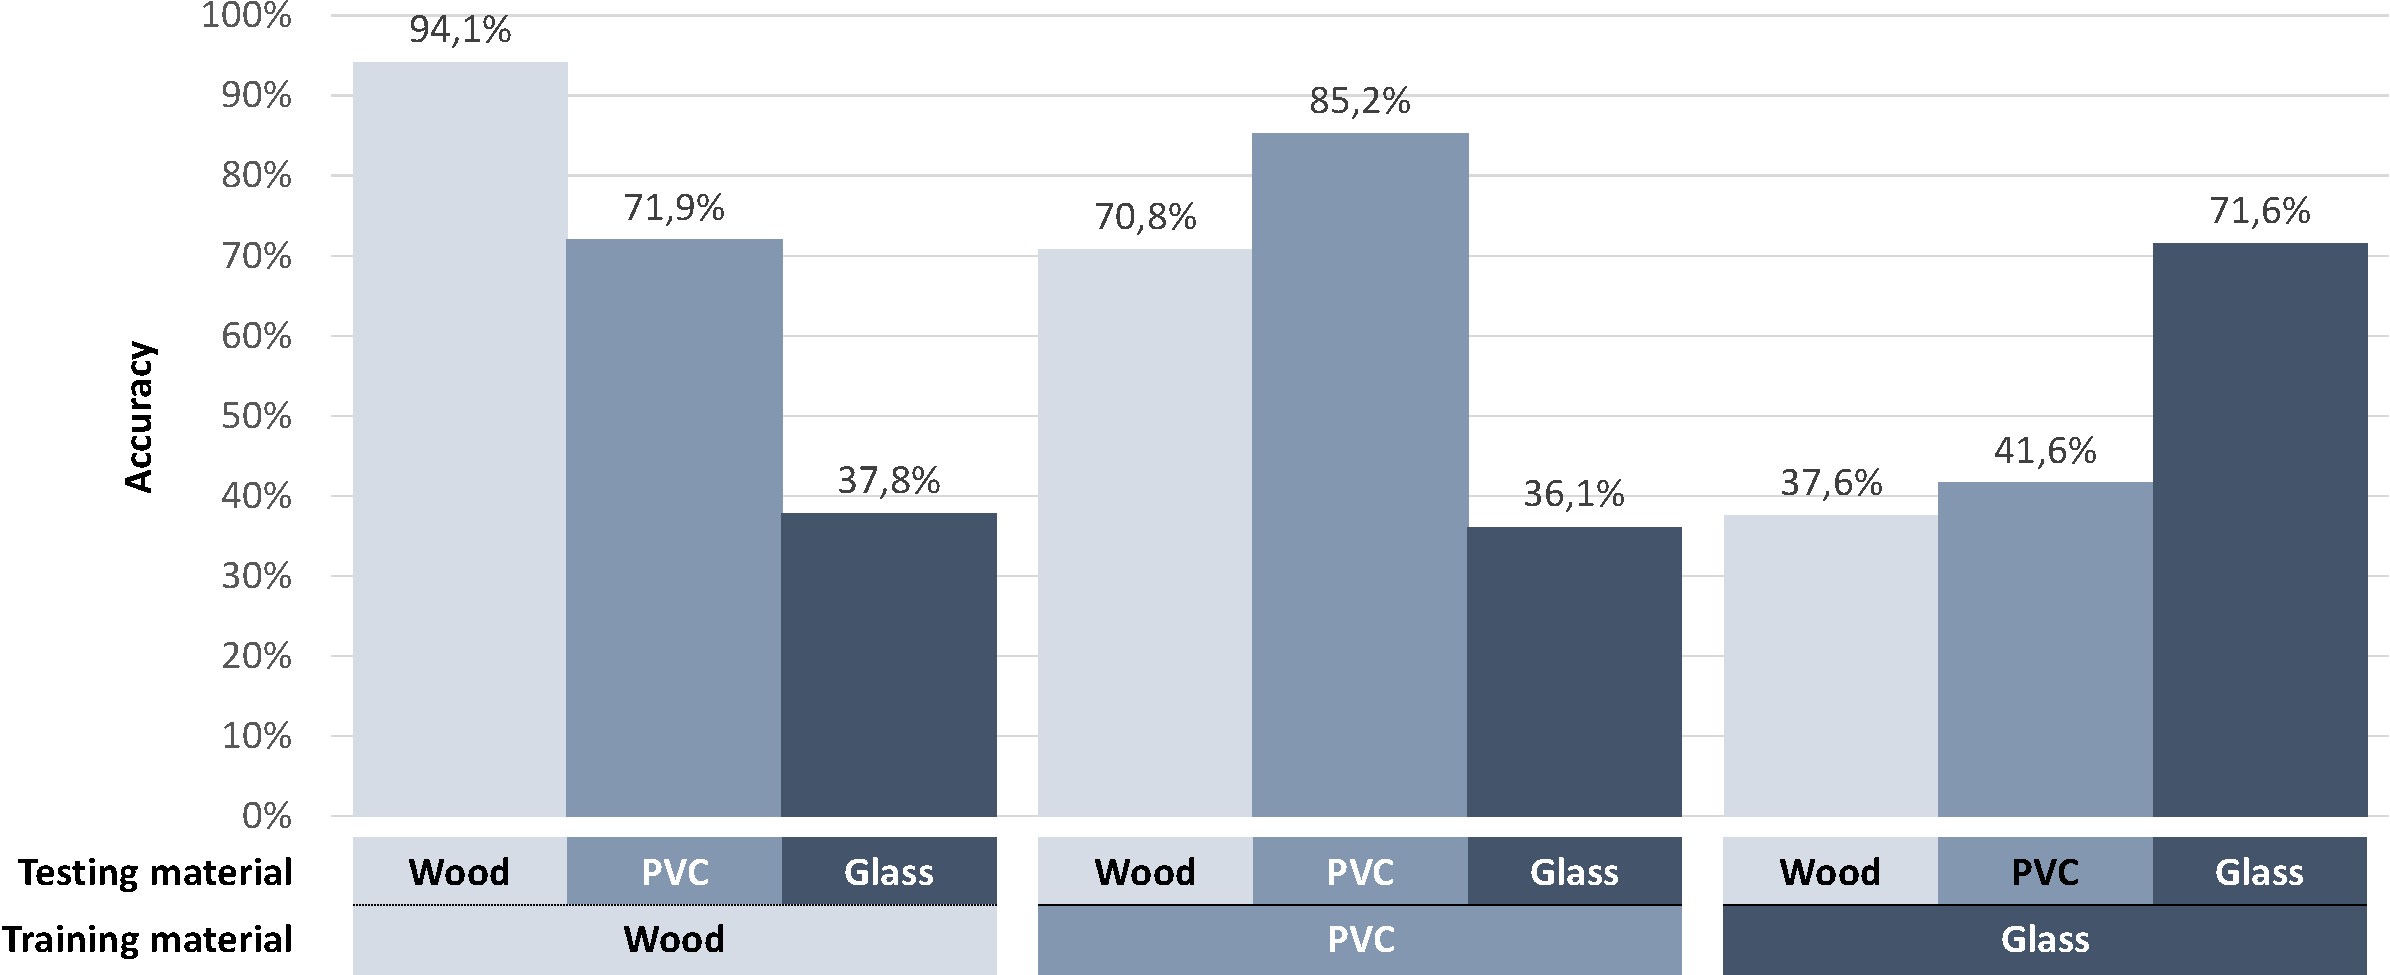
\includegraphics[width=\linewidth]{Figures/RadarExperiments/Datasets/ThroughMaterials/through-materials-results-timegating.pdf}
        \vspace{-12pt}
        \caption{Time gating stage.}
        \label{fig:radar-experiments:through-materials:results:timegating}
    \end{subfigure}

    \begin{subfigure}{\linewidth}
        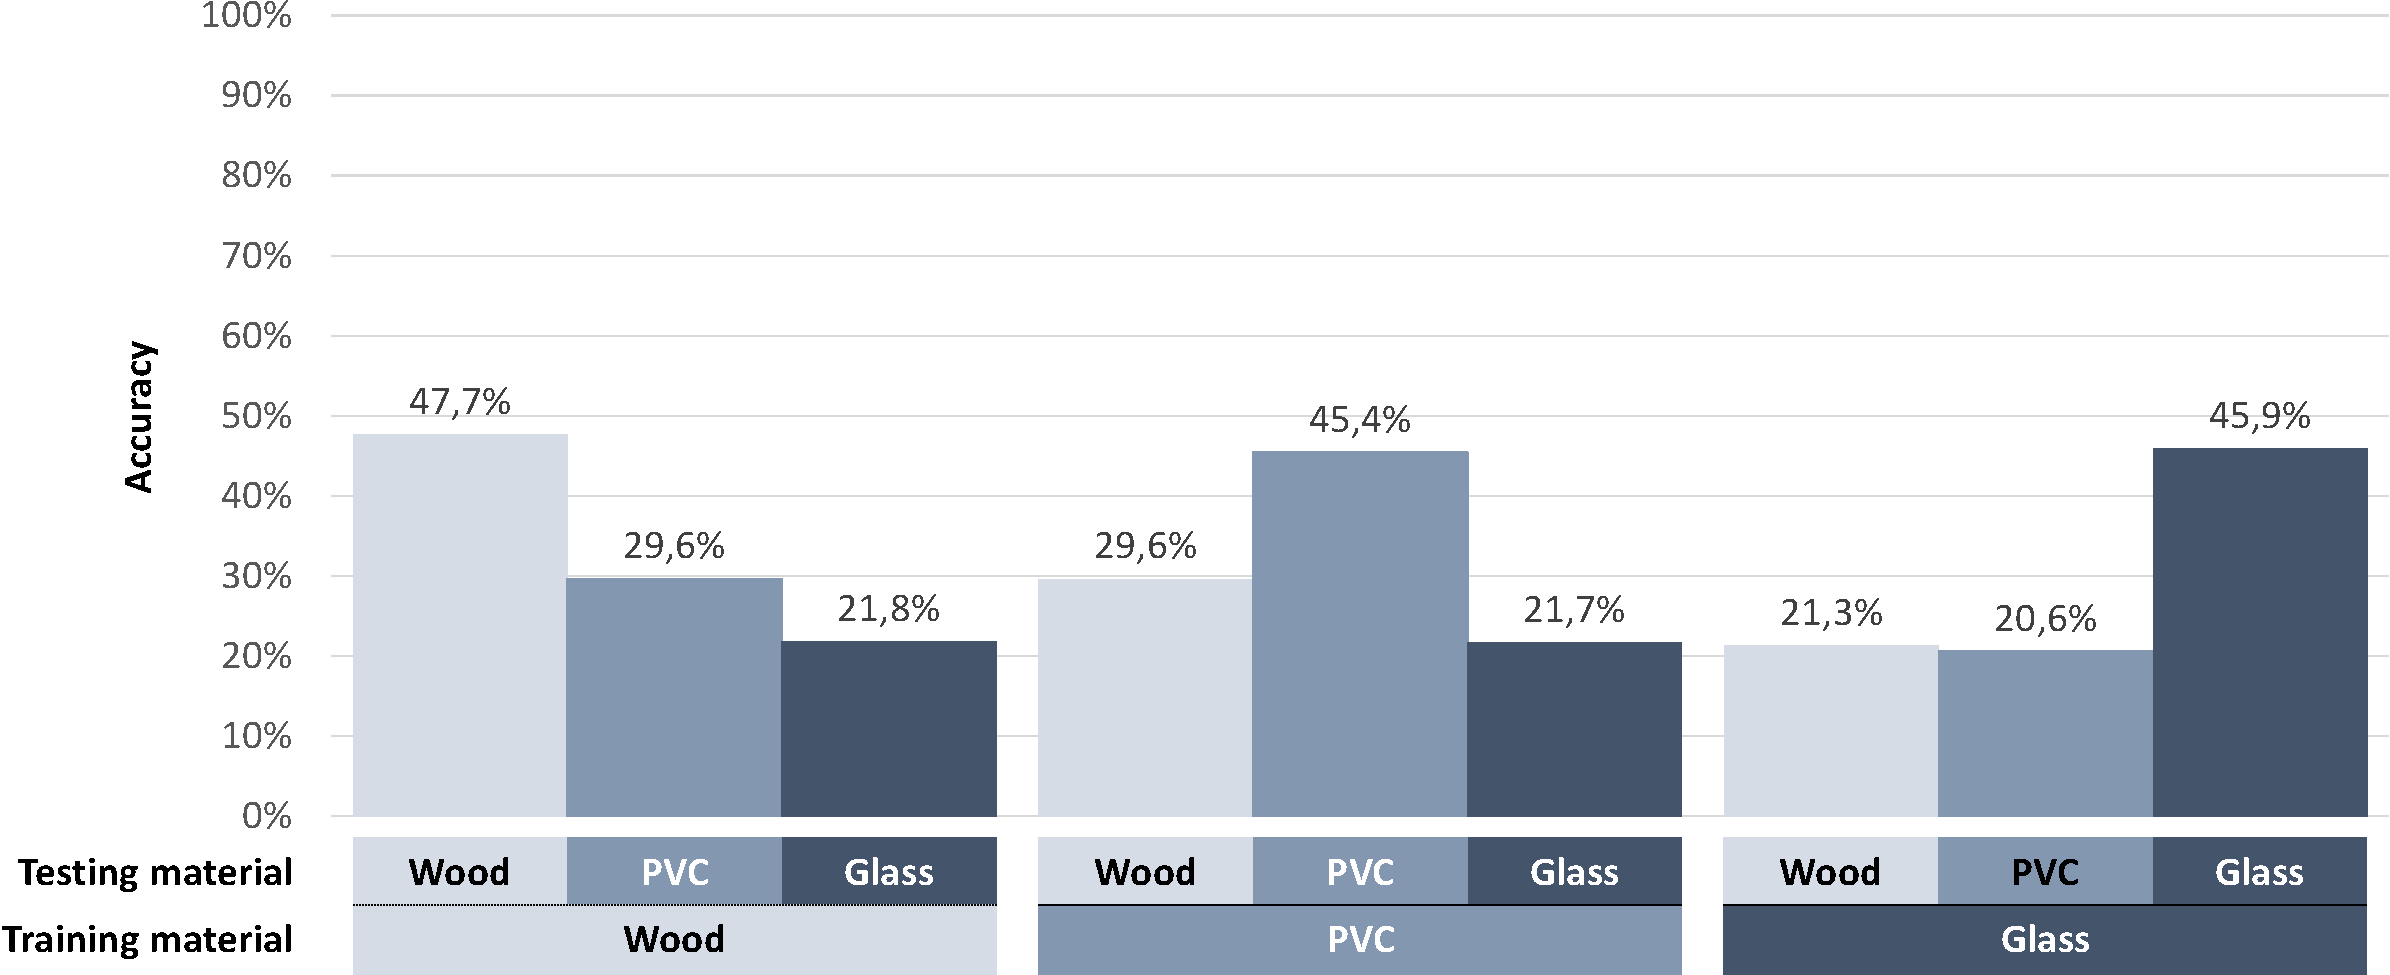
\includegraphics[width=\linewidth]{Figures/RadarExperiments/Datasets/ThroughMaterials/through-materials-results-filtering.pdf}
        \vspace{-12pt}
        \caption{Filtering stage.}
        \label{fig:radar-experiments:through-materials:results:filtering}
    \end{subfigure}
    \caption{Average gesture recognition accuracy in the best configuration for each combination of training and testing materials in the user-dependent scenario at two stages of the pipeline.}
    \label{fig:radar-experiments:through-materials:results}
    \vspace{-28pt}
\end{figure}

\subsubsection{Intra-material} \label{sec:radar-experiments:through-materials:results:intra-material}
Intra-material testing was conducted in three scenarios: user-dependent, user-independent, and mixed.
%
\fig~\ref{fig:radar-experiments:through-materials:wood-samples}, \ref{fig:radar-experiments:through-materials:pvc-samples}, and~\ref{fig:radar-experiments:through-materials:glass-samples} depict the evolution of accuracy with respect to the number of sampling points in user-dependent and user-independent scenarios for the wood, PVC, and glass training/testing materials, respectively.
%
Similarly, \fig~\ref{fig:radar-experiments:through-materials:wood-confusion}, \ref{fig:radar-experiments:through-materials:pvc-confusion}, and~\ref{fig:radar-experiments:through-materials:glass-confusion} show the confusion matrices of the best configurations in user-dependent and user-independent scenarios for the wood, PVC, and glass training/testing materials, respectively.

\begin{figure}[!t]
    \begin{subfigure}{.49\textwidth}
        \centering
        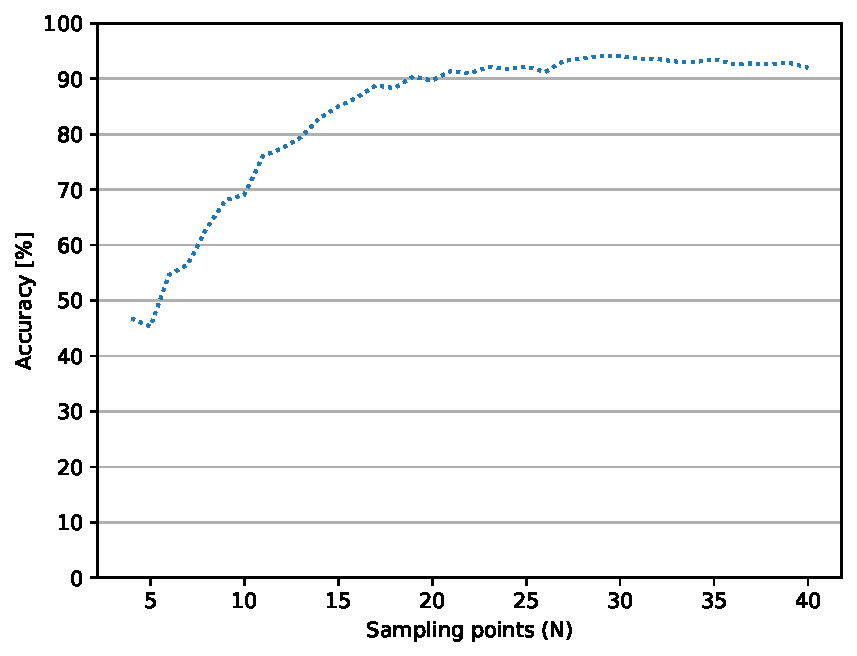
\includegraphics[width=.99\linewidth]{Figures/RadarExperiments/Datasets/ThroughMaterials/Wood/samples-timegating-ud.pdf}
        \vspace{-5pt}
        \captionsetup{width=.99\linewidth}
        \caption{Time gating UD \\ $\splitatcommas{AP{=}(1, 2, 3, 4, 5, 6, 7, 8, 9, 10, 11, 12)}$.}
        \label{fig:radar-experiments:through-materials:wood-samples:timegating-ud}
    \end{subfigure}
    \begin{subfigure}{.49\textwidth}
        \centering
        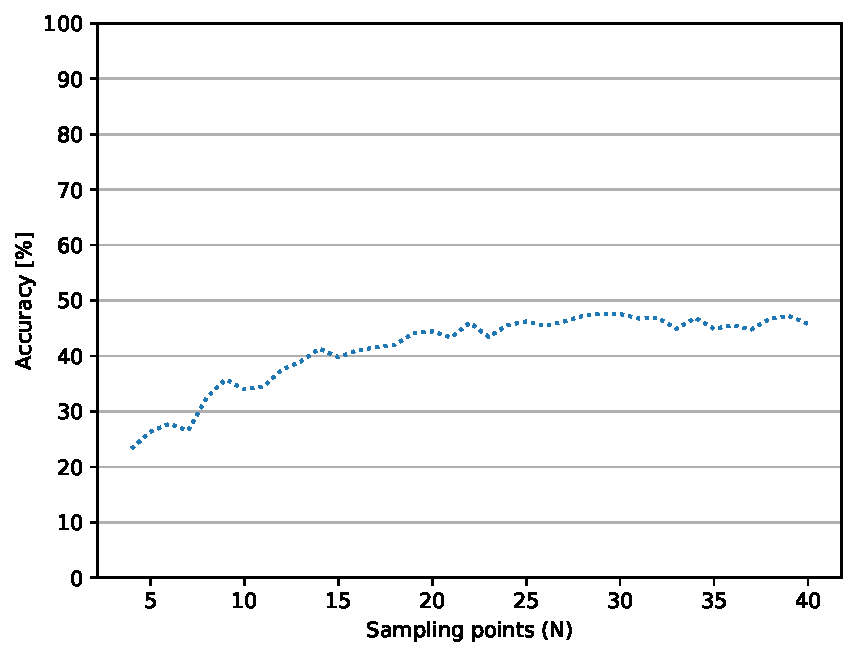
\includegraphics[width=.99\linewidth]{Figures/RadarExperiments/Datasets/ThroughMaterials/Wood/samples-filtering-ud.pdf}  
        \vspace{-5pt}
        \captionsetup{width=.99\linewidth}
        \caption{Filtering UD \\ $\splitatcommas{AP{=}(1, 2, 3, 4, 5, 6, 7, 8, 9, 10, 11, 12)}$.}
        \label{fig:radar-experiments:through-materials:wood-samples:filtering-ud}
    \end{subfigure}
  
    \begin{subfigure}{.49\textwidth}
        \centering
        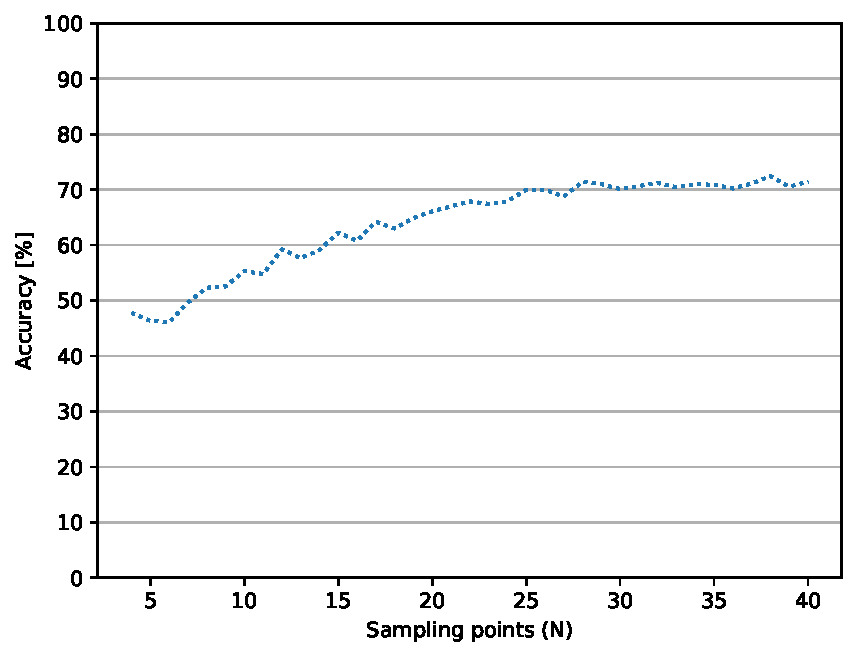
\includegraphics[width=.99\linewidth]{Figures/RadarExperiments/Datasets/ThroughMaterials/Wood/samples-timegating-ui.pdf}
        \vspace{-5pt}
        \captionsetup{width=.99\linewidth}
        \caption{Time gating UI \\ $\splitatcommas{AP{=}(1, 2, 3, 4, 5, 6, 7, 8, 9, 10, 11, 12)}$.}
        \label{fig:radar-experiments:through-materials:wood-samples:timegating-ui}
    \end{subfigure}
    \begin{subfigure}{.49\textwidth}
        \centering
        \includegraphics[width=.99\linewidth]{Figures/RadarExperiments/Datasets/ThroughMaterials/Wood/samples-filtering-ui.pdf}  
        \vspace{-5pt}
        \captionsetup{width=.99\linewidth}
        \caption{Filtering UI \\ $\splitatcommas{AP{=}(1, 2, 3, 6, 8, 9)}$.}
        \label{fig:radar-experiments:through-materials:wood-samples:filtering-ui}
    \end{subfigure}
  
    \vspace{-6pt}
    \caption{The accuracy of Jackknife with respect to the number of sampling points for the best-performing set of antenna pairs when using wood data for training and testing in a user-dependent (top) and user-independent scenario (bottom).}
    \label{fig:radar-experiments:through-materials:wood-samples}
\end{figure}

\paragraph{Time gating.}

% User-dependent
\fig~\ref{fig:radar-experiments:through-materials:results:timegating} shows the average accuracy achieved by the best configuration for each combination of training and testing material with data from the time-gating stage in the user-dependent scenario.
%
Overall, we observed that the average accuracy increased rather smoothly with the number of sampling points, plateauing at around 93\%, 84\%, and 70\% for the wood, PVC, and glass, respectively.
% Wood
The best configuration achieved 94.1\% accuracy for the wood ($N{=}29$, $\splitatcommas{AP{=}(1, 2, 3, 4, 5, 6, 7, 8, 9, 10, 11, 12)}$), with all but one gesture correctly recognized more than 90\% of the time. Average execution time was rather short, at 16.3 ms.
%
We noticed some confusion between gestures a and o (open hand and push fist), as well as between b and p (close hand and push palm). In both cases, the gestures start with a similar hand pose and motion. For instance, ``open hand'' starts with the hand closed and moving slightly towards the radar before opening the hand, which is similar to the ``push fist'' gesture.
% PVC and glass
Average accuracy dropped for the PVC and glass, at 85.2\% ($N{=}40$, $\splitatcommas{AP{=}(4, 5, 7, 10, 11, 12)}$), and 71.6\% ($N{=}38$, $\splitatcommas{AP{=}(1, 2, 3, 6, 8, 9)}$), respectively.
%
As for the wood, gesture a (resp. b) was often confused with gesture o (resp. p).
%
In addition, we noticed some confusion between gestures a, b, and c (open/close/open then close hand), and between gestures o and p (push fist/palm), especially for the glass. This indicates that differences in signal amplitude become harder to identify as the signal-to-noise ratio decreases.
%
With the glass, we also observed some confusion between swipes (h, i, j) and ``open/close/open then close hand'' (a, b, c). This was also observed in the first experiment (Section~\ref{sec:radar-experiments:sensors:results}) and probably stems from an inability of the radar to accurately distinguish between moving the hand in the plane orthogonal to the radar beam and changing its radar cross-section.

%User-independent
Average accuracy in the user-independent scenario was lower but behaved similarly to the user-dependent scenario, plateauing at around 70\%, 63\%, and 55\% for the wood, PVC, and glass, respectively. This is better than in the second experiment (Section~\ref{sec:radar-experiments:gesture-subsets:results}), which may be explained by the smaller set of gestures, the larger number of participants, and the use of time-domain data.
% Wood
The best configuration achieved 72.4\% accuracy for the wood ($N{=}38$, $\splitatcommas{AP{=}(1, 2, 3, 4, 5, 6, 7, 8, 9, 10, 11, 12)}$). The average execution time was very long, at 342.2 ms.
%
Our observations are mostly similar to the user-dependent scenario, with some confusion between gestures a and o (open hand and push fist), b and p (close hand and push palm), o and p (push fist/palm), j and k (swipe up/down),  as well as between h and i (swipe right/left).
% PVC and glass
Average accuracy also dropped for the best configurations of the PVC and glass, at 64.9\% ($N{=}34$, $\splitatcommas{AP{=}(4, 5, 7, 10, 11, 12)}$), and 55.7\% ($N{=}34$, $\splitatcommas{AP{=}(1, 2, 3, 6, 8, 9)}$), respectively. The corresponding confusion matrices are very similar to the wood, albeit with lower accuracy.

\begin{figure}[!t]
    \begin{subfigure}{.49\textwidth}
        \centering
        \includegraphics[width=.99\linewidth]{Figures/RadarExperiments/Datasets/ThroughMaterials/Wood/confusion-timegating-ud.pdf}
        \vspace{-15pt}
        \captionsetup{width=.99\linewidth}
        \caption{Time gating UD $N{=}29$, \\ $\splitatcommas{AP{=}(1, 2, 3, 4, 5, 6, 7, 8, 9, 10, 11, 12)}$.}
        \label{fig:radar-experiments:through-materials:wood-confusion:timegating-ud}
    \end{subfigure}
    \begin{subfigure}{.49\textwidth}
        \centering
        \includegraphics[width=.99\linewidth]{Figures/RadarExperiments/Datasets/ThroughMaterials/Wood/confusion-filtering-ud.pdf}
        \vspace{-15pt}
        \captionsetup{width=.99\linewidth}
        \caption{Filtering UD $N{=}29$, \\ $\splitatcommas{AP{=}(1, 2, 3, 4, 5, 6, 7, 8, 9, 10, 11, 12)}$.}
        \label{fig:radar-experiments:through-materials:wood-confusion:filtering-ud}
    \end{subfigure}

    \begin{subfigure}{.49\textwidth}
        \centering
        \includegraphics[width=.99\linewidth]{Figures/RadarExperiments/Datasets/ThroughMaterials/Wood/confusion-timegating-ui.pdf}  
        \vspace{-15pt}
        \captionsetup{width=.99\linewidth}
        \caption{Time gating UI $N{=}38$, \\ $\splitatcommas{AP{=}(1, 2, 3, 4, 5, 6, 7, 8, 9, 10, 11, 12)}$.}
        \label{fig:radar-experiments:through-materials:wood-confusion:timegating-ui}
    \end{subfigure}
    \begin{subfigure}{.49\textwidth}
        \centering
        \includegraphics[width=.99\linewidth]{Figures/RadarExperiments/Datasets/ThroughMaterials/Wood/confusion-filtering-ui.pdf}
        \vspace{-15pt}
        \captionsetup{width=.99\linewidth}
        \caption{Filtering UI $N{=}30$, \\ $\splitatcommas{AP{=}(1, 2, 3, 6, 8, 9)}$.}
        \label{fig:radar-experiments:through-materials:wood-confusion:filtering-ui}
    \end{subfigure}
    
    % \vspace{-6pt}
    \caption{Normalized confusion matrices for the best configuration at two stages of the pipeline in user-dependent (top) and user-independent scenarios (bottom) when using wood data for training and testing. The values in each cell are represented as percentages.}
    \label{fig:radar-experiments:through-materials:wood-confusion}
\end{figure}

\paragraph{Filtering.}
\fig~\ref{fig:radar-experiments:through-materials:results:filtering} depicts the average accuracy achieved by the best configuration for each combination of training and testing material with data from the filtering stage in the user-dependent scenario.
%
Accuracy dropped significantly compared to time-domain data from the time gating stage but still increased with the number of sampling points, plateauing at around 46\% for the wood and 43\% for the PVC and glass.
% Wood, PVC, and glass
The best configurations for the wood, PVC, and glass all performed similarly, reaching 47.7\% ($N{=}38$, $\splitatcommas{AP{=}(1, 2, 3, 4, 5, 6, 7, 8, 9, 10, 11, 12)}$), 45.4\% ($N{=}32$, $\splitatcommas{AP{=}(1, 2, 3, 4, 5, 6, 7, 8, 9, 10, 11, 12)}$), and 45.9\% ($N{=}23$, $\splitatcommas{AP{=}(1, 2, 3, 4, 5, 6, 7, 8, 9, 10, 11, 12)}$), respectively. Execution time was very short at 0.6 ms for the wood.

Accuracy in the user-independent scenario was slightly higher and similar across all materials, reaching 48.7\% ($N{=}30$, $\splitatcommas{AP{=}(1, 2, 3, 6, 8, 9)}$), 49.1\% ($N{=}38$, $\splitatcommas{AP{=}(1, 2, 3, 6, 8, 9)}$), and 51.1\% ($N{=}36$, $\splitatcommas{AP{=}(1, 2, 3, 4, 5, 6, 7, 8, 9, 10, 11, 12)}$), for the wood, PVC, and glass, respectively. The average execution time was longer at 7.7 ms for the wood.

The confusion matrices in both scenarios are very similar and our observations from the time gating stage are also valid for this stage. 


% % User-dependent
% % Wood
% % Time gating
% 94.1\%, 16.3ms ($N{=}29$, $\splitatcommas{AP{=}(1, 2, 3, 4, 5, 6, 7, 8, 9, 10, 11, 12)}$)
% % Filtering
% 47.7\%, 0.6ms ($N{=}29$, $\splitatcommas{AP{=}(1, 2, 3, 4, 5, 6, 7, 8, 9, 10, 11, 12)}$)

% % PVC
% % Time gating
% 85.2\%, 11.8ms ($N{=}40$, $\splitatcommas{AP{=}(4, 5, 7, 10, 11, 12)}$)
% % Filtering
% 45.4\%, 0.6ms ($N{=}32$, $\splitatcommas{AP{=}(1, 2, 3, 4, 5, 6, 7, 8, 9, 10, 11, 12)}$)

% % Glass
% % Time gating
% 71.6\%, 11.2ms ($N{=}38$, $\splitatcommas{AP{=}(1, 2, 3, 6, 8, 9)}$)
% % Filtering
% 45.9\%, 0.4ms ($N{=}23$, $\splitatcommas{AP{=}(1, 2, 3, 4, 5, 6, 7, 8, 9, 10, 11, 12)}$)

% User-independent
% Wood
% Time gating
% 72.4\%, 342.2ms ($N{=}38$, $\splitatcommas{AP{=}(1, 2, 3, 4, 5, 6, 7, 8, 9, 10, 11, 12)}$)
% % Filtering
% 48.7\%, 7.7ms ($N{=}30$, $\splitatcommas{AP{=}(1, 2, 3, 6, 8, 9)}$)

% % PVC
% % Time gating
% 64.9\%, 152.0ms ($N{=}34$, $\splitatcommas{AP{=}(4, 5, 7, 10, 11, 12)}$)
% % Filtering
% 49.1\%, 9.2ms ($N{=}38$, $\splitatcommas{AP{=}(1, 2, 3, 6, 8, 9)}$)

% % Glass
% % Time gating
% 55.7\%, 154.3ms ($N{=}34$, $\splitatcommas{AP{=}(1, 2, 3, 6, 8, 9)}$)
% % Filtering
% 51.1\%, 11.7ms ($N{=}36$, $\splitatcommas{AP{=}(1, 2, 3, 4, 5, 6, 7, 8, 9, 10, 11, 12)}$)

\subsubsection{Inter-material} \label{sec:radar-experiments:through-materials:results:inter-material}
The inter-material testing was only conducted in a user-dependent scenario.
%
\fig~\ref{fig:radar-experiments:through-materials:wood-pvc-samples}, \ref{fig:radar-experiments:through-materials:pvc-wood-samples}, \ref{fig:radar-experiments:through-materials:wood-glass-samples}, \ref{fig:radar-experiments:through-materials:glass-wood-samples},\ref{fig:radar-experiments:through-materials:pvc-glass-samples}, and~\ref{fig:radar-experiments:through-materials:glass-pvc-samples} depict the evolution of accuracy with respect to the number of sampling points for the wood+PVC, PVC+wood, wood+glass, glass+wood, PVC+glass, and glass+PVC training/testing materials, respectively.
%
Similarly, \fig~\ref{fig:radar-experiments:through-materials:wood-pvc-confusion}, \ref{fig:radar-experiments:through-materials:pvc-wood-confusion}, \ref{fig:radar-experiments:through-materials:wood-glass-confusion}, \ref{fig:radar-experiments:through-materials:glass-wood-confusion},\ref{fig:radar-experiments:through-materials:pvc-glass-confusion}, and~\ref{fig:radar-experiments:through-materials:glass-pvc-confusion} show the confusion matrices of the best configurations for the wood+PVC, PVC+wood, wood+glass, glass+wood, PVC+glass, and glass+PVC conditions, respectively. 

\paragraph{Time gating.}
\fig~\ref{fig:radar-experiments:through-materials:results:filtering} depicts the average accuracy achieved by the best configuration for each combination of training and testing material with data from the time gating stage.
% Wood + PVC, PVC + Wood
The results for the wood+PVC and PVC+wood combinations of training and testing materials are similar to those of the intra-material testing in the user-dependent scenario but with slightly lower accuracy. 
%
The best configurations reached 71.9\% ($N{=}34$, $\splitatcommas{AP{=}(4, 5, 7, 10, 11, 12)}$) and 70.8\% accuracy ($N{=}35$, $\splitatcommas{AP{=}(4, 5, 7, 10, 11, 12)}$) for wood+PVC and PVC+wood, respectively.
%
The corresponding confusion matrices are very similar to those of the intra-dataset testing, and our observations are thus still valid here. 
% Wood + glass, Glass + wood, PVC + glass, Glass + PVC
Accuracy for wood+glass, glass+wood, pvc+glass and glass+pvc combinations of materials dropped drastically, at 37.8\% ($N{=}40$, $\splitatcommas{AP{=}(1, 2, 3, 6, 8, 9)}$), 37.6\% ($N{=}29$, $\splitatcommas{AP{=}(1, 2, 3, 6, 8, 9)}$), 36.1\% ($N{=}37$, $\splitatcommas{AP{=}(1, 2, 3, 6, 8, 9)}$), and 41.6\% ($N{=}37$, $\splitatcommas{AP{=}(4, 5, 7, 10, 11, 12)}$), respectively.
%
This drop in accuracy seems to indicate that, despite the normalization applied by our processing pipeline, radar signals recorded through the glass were not comparable to those recorded through the wood and PVC. This may have been a consequence of the high relative permittivity of the glass which caused more energy to be reflected at the interface between air and glass. This, in turn, resulted in a lower signal-to-noise ratio. 
%
The smaller relative permittivity of wood and PVC resulted in a higher signal-to-noise ratio and thus more comparable radar signatures.


\paragraph{Filtering.}
\fig~\ref{fig:radar-experiments:through-materials:results:filtering} depicts the average accuracy achieved by the best configuration for each combination of training and testing material with data from the filtering stage.
% Wood + PVC, PVC + Wood
The results are similar to those obtained with data from the time gating stage, but with even lower accuracy, reaching only 29.6\% accuracy with the wood+pvc ($N{=}34$, $\splitatcommas{AP{=}(1, 2, 3, 4, 5, 6, 7, 8, 9, 10, 11, 12)}$) and pvc+wood materials ($N{=}26$, $\splitatcommas{AP{=}(1, 2, 3, 4, 5, 6, 7, 8, 9, 10, 11, 12)}$).
%
Because of the very low accuracy, it is difficult to draw any conclusion from the corresponding confusion matrices.
% Wood + glass, Glass + wood, PVC + glass, Glass + PVC
Accuracy for wood+glass, glass+wood, pvc+glass and glass+pvc combinations of materials dropped by nearly 10\%, at 21.8\% ($N{=}21$, $\splitatcommas{AP{=}(1, 2, 3, 6, 8, 9)}$), 21.3\% ($N{=}21$, $\splitatcommas{AP{=}(1, 2, 3, 6, 8, 9)}$), 21.7\% ($N{=}20$, $\splitatcommas{AP{=}(1, 2, 3, 6, 8, 9)}$), and 20.6\% ($N{=}36$, $\splitatcommas{AP{=}(1, 2, 3, 6, 8, 9)}$), respectively.
%
Similarly to the time gating stage, the low accuracy could be explained by the lower signal-to-noise ratio of the signals recorded through glass, which may have caused the inversion process to fail more often than for the other materials.


\begin{figure}[t]
    \begin{subfigure}{.49\textwidth}
        \centering
        \includegraphics[width=.99\linewidth]{Figures/RadarExperiments/Datasets/ThroughMaterials/Wood+PVC/samples-timegating-ud.pdf}
        \vspace{-15pt}
        \captionsetup{width=.99\linewidth}
        \caption{Time gating \\ $\splitatcommas{AP{=}(4, 5, 7, 10, 11, 12)}$.}
        \label{fig:radar-experiments:through-materials:wood-pvc-samples:timegating-ud}
    \end{subfigure}
    \begin{subfigure}{.49\textwidth}
        \centering
        \includegraphics[width=.99\linewidth]{Figures/RadarExperiments/Datasets/ThroughMaterials/Wood+PVC/samples-filtering-ud.pdf}  
        \vspace{-15pt}
        \captionsetup{width=.99\linewidth}
        \caption{Filtering \\ $\splitatcommas{AP{=}(1, 2, 3, 4, 5, 6, 7, 8, 9, 10, 11, 12)}$.}
        \label{fig:radar-experiments:through-materials:wood-pvc-samples:filtering-ud}
    \end{subfigure}
  
    % \vspace{-6pt}
    \caption{The accuracy of Jackknife with respect to the number of sampling points for the best-performing set of antenna pairs when using wood data for training and PVC data for testing in a user-dependent scenario.}
    \label{fig:radar-experiments:through-materials:wood-pvc-samples}
\end{figure}

\begin{figure}[ht]
    \begin{subfigure}{.49\textwidth}
        \centering
        \includegraphics[width=.99\linewidth]{Figures/RadarExperiments/Datasets/ThroughMaterials/Wood+PVC/confusion-timegating-ud.pdf}
        \vspace{-15pt}
        \captionsetup{width=.99\linewidth}
        \caption{Time gating $N{=}34$, \\ $\splitatcommas{AP{=}(4, 5, 7, 10, 11, 12)}$.}
        \label{fig:radar-experiments:through-materials:wood-pvc-confusion:timegating-ud}
    \end{subfigure}
    \begin{subfigure}{.49\textwidth}
        \centering
        \includegraphics[width=.99\linewidth]{Figures/RadarExperiments/Datasets/ThroughMaterials/Wood+PVC/confusion-filtering-ud.pdf}
        \vspace{-15pt}
        \captionsetup{width=.99\linewidth}
        \caption{Filtering $N{=}34$, \\ $\splitatcommas{AP{=}(1, 2, 3, 4, 5, 6, 7, 8, 9, 10, 11, 12)}$.}
        \label{fig:radar-experiments:through-materials:wood-pvc-confusion:filtering-ud}
    \end{subfigure}
    
    % \vspace{-6pt}
    \caption{Normalized confusion matrices for the best configuration at two stages of the pipeline in the user-dependent scenario when using wood data for training and PVC data for testing. The values in each cell are represented as percentages.}
    \label{fig:radar-experiments:through-materials:wood-pvc-confusion}
\end{figure}

% % Wood-PVC
% % Time gating
% 71.9\%, 10.9ms ($N{=}34$, $\splitatcommas{AP{=}(4, 5, 7, 10, 11, 12)}$)
% % Filtering
% 29.6\%, 1.0ms ($N{=}34$, $\splitatcommas{AP{=}(1, 2, 3, 4, 5, 6, 7, 8, 9, 10, 11, 12)}$)

% % PVC-Wood
% % Time gating
% 70.8\%, 11.0ms ($N{=}35$, $\splitatcommas{AP{=}(4, 5, 7, 10, 11, 12)}$)
% % Filtering
% 29.6\%, 0.5ms ($N{=}26$, $\splitatcommas{AP{=}(1, 2, 3, 4, 5, 6, 7, 8, 9, 10, 11, 12)}$)

% % Wood-Glass
% % Time gating
% 37.8\%, 12.0ms ($N{=}40$, $\splitatcommas{AP{=}(1, 2, 3, 6, 8, 9)}$)
% % Filtering
% 21.8\%, 0.3ms ($N{=}21$, $\splitatcommas{AP{=}(1, 2, 3, 6, 8, 9)}$)

% % Glass-Wood
% % Time gating
% 37.6\%, 8.5ms ($N{=}29$, $\splitatcommas{AP{=}(1, 2, 3, 6, 8, 9)}$)
% % Filtering
% 21.3\%, 0.3ms ($N{=}21$, $\splitatcommas{AP{=}(1, 2, 3, 6, 8, 9)}$)

% % PVC-Glass
% % Time gating
% 36.1\%, 12.0ms ($N{=}37$, $\splitatcommas{AP{=}(1, 2, 3, 6, 8, 9)}$)
% % Filtering
% 21.7\%, 0.3ms ($N{=}20$, $\splitatcommas{AP{=}(1, 2, 3, 6, 8, 9)}$)

% % Glass-PVC
% % Time gating
% 41.6\%, 10.7ms ($N{=}37$, $\splitatcommas{AP{=}(4, 5, 7, 10, 11, 12)}$)
% % Filtering
% 20.6\%, 0.5ms ($N{=}36$, $\splitatcommas{AP{=}(1, 2, 3, 6, 8, 9)}$)


%--------------------------------------------------------------------------------%
\subsection{Summary} \label{sec:radar-experiments:through-materials:discussion}
This experiment demonstrated that a relatively inexpensive radar like the Walabot could perform relatively well through some types of materials, including wood and PVC. In addition, our signal-processing pipeline was able to normalize the signals from the two materials, achieving a fairly high accuracy of around 71\% across these materials.
The results of Leiva \etal's study about radar sensing through fabric~\cite{Leiva:2020} suggest that training the gesture recognition algorithm on a larger set of samples without material obstruction could further enhance accuracy across all tested materials. This avenue would be worth investigating in future research, as combining this technique with the data normalization applied by our pipeline could lead to even greater gesture recognition accuracy through different materials.
%
The higher relative permittivity of the glass compared to the other materials resulted in a lower accuracy. While the average accuracy still reached 71.6\% in the user-dependent scenario when using glass data for training and testing, it dropped to around 38\% when mixing glass with another material. This indicates that our processing pipeline could not properly normalize signals recorded through the glass, probably because of the lower signal-to-noise ratio. Other radar systems operating at a different power level and/or frequency range may alleviate this issue.
%
Finally, our results were more stable with respect to the number of sampling points than in the previous experiments, suggesting that the time-domain data we used in this experiment may be better suited to gesture recognition than frequency-domain data.

%================================================================================%
\section{Discussion and Implications for Design} \label{sec:radar-experiments:discussion}
In this section, we draw ten implications from our three experiments for the design of hand gesture interaction with radar sensors. These implications are categorized into four key areas: (1) radar systems (R1), (2) gesture sets (G1-G5), (3) signal processing (S1-S2), and (4) environment of interaction (E1-E2).

\paragraph{R1. Use multiple antennas with enough separation.}
Our first experiment (Section~\ref{sec:radar-experiments:sensors:results:walabot}) showed that taking advantage of multiple pairs of antennas could improve gesture recognition accuracy, as more information was captured that could help differentiate between similar gestures. Overall, the number of antennas seemed to be a more relevant parameter than the quality of the antennas, especially when using data from the full-wave inversion and filtering stages. 

\begin{figure}
    \centering
    \includegraphics[width=.4\linewidth]{Figures/RadarExperiments/Discussion/pipeline-limitations-size.pdf}
    \caption{Examples of variations in hand position and surface.}
    \label{fig:radar-experiments:discussion:elevation}
\end{figure}

\paragraph{G1. Collect gestures from multiple users.}
Hands can vary widely in size and surface area between users. The length of the hand can range from 15 to 30 cm (5.9 to 11.8 in) and the circumference of the hand from 15 to 28 cm (5.9 to 11.02 in), giving an idea of the potential surface range. Hand and palm surface areas vary with gender, age, and morphology. For example, \cite{Goker:2017} reported that the average hand surface area for Turkish women and men is \textit{M}{=}158.34 $cm^2$ (\textit{SD}{=}14.76 $cm^2$) and \textit{M}{=}127.87 $cm^2$ (\textit{SD}{=}14.75 $cm^2$), respectively, and palm surface area \textit{M}{=}63.91 $cm^2$ (\textit{M}{=}11.84 $cm^2$) and \textit{M}{=}82.98 $cm^2$ (\textit{SD}{=}10.74 $cm^2)$, respectively. 
Variations in the hand surface area result in variations in the radar signal that should be taken into account to ensure high recognition accuracy, especially for the user-independent scenario. Other parameters can equally vary between different users, such as arm length and position relative to the radar (\eg elevation, distance), which may also result in signal variations (\fig~\ref{fig:radar-experiments:discussion:elevation}). Gesture training sets for user-independent recognition should include samples produced by a variety of users.

\paragraph{G2. Support user customization.}
Our testing showed that gesture recognition accuracy in user-independent scenarios was too low to be usable in real applications. Conversely, our system performed very well in user-dependent and even mixed scenarios.
%
Using small gesture sets that contain training samples produced by the current user of the system thus seems to be the key to achieving high gesture recognition accuracy. The ability of our system to work with very few training samples facilitates this, as it takes only a few minutes for users to generate their own gesture set.
%
In addition, user-defined gestures usually result in higher satisfaction and memorability~\cite{Nacenta:2013}.

\paragraph{G3. Favor gestures with motion parallel to the radar beam.}
As the angular resolution of a radar is significantly lower than its range resolution, it is easier to recognize gestures that are performed in a parallel plane with respect to the radar than in other configurations, such as the orthogonal plane. As a negative example, the ``swipe left/right/up/down'' and ``open/close hand'' gestures are more difficult to differentiate, especially with only one pair of antennas (Section~\ref{sec:radar-experiments:sensors:results:horn}). As a positive example, ``push with palm/fist'' will be easier to differentiate from other gestures (\eg ``pull''), even with one antenna pair due to the relatively good range resolution of the radar.

\paragraph{G4. Favor gestures with a highly differentiable surface of exposure.} 
For example, in the user-dependent scenario, there was little to no confusion between the ``push with palm'' and ``push with fist'' gestures (Fig.~\ref{fig:radar-experiments:sensors:horn-confusion:bgsub}, \ref{fig:radar-experiments:sensors:walabot-confusion:bgsub}, \ref{fig:radar-experiments:confusion-exp1-UD-timegating}) because the palm has a larger exposure surface than the fist, resulting in a larger amplitude of the received radar signal. This difference in amplitude can be used by a recognizer to differentiate between the two gestures. On the other hand, gestures such as ``extend one/two/three/four fingers'' were less accurately recognized, especially in the user-independent scenario (Fig.~\ref{fig:radar-experiments:confusion-exp1-UI-timegating}) because the changes in their surfaces of exposure were relatively small.

\paragraph{G5. Select gestures based on the level of criticality of your application.}
For non-critical applications (\eg interacting with a TV at home), gestures with lower accuracy, such as ``open/close/open then close hand'' and ``extend one/two/three/four fingers'', may be selected if they are well suited to perform a specific action. In such applications, an incorrect result from the recognizer would only impact the user experience of the application.
%
For safety-critical applications, such as performing high-precision medical procedures, developers should rely on small gesture sets composed exclusively of gestures that can be recognized with very high accuracy (> 99\%). To guarantee high accuracy, it is strongly advised to train the system with data from the same person(s) that would use the system, as an incorrectly recognized gesture in these applications could have life-threatening consequences. 
    
% \paragraph{\textbf{I6. Favor the most accurately recognized gestures.}} 
% Priority should be given to gestures that are the most accurately recognized. Positive examples for the Walabot are gestures no. 1 to 4, 7, 10, and 11 with more than 70\% recognition accuracy rates.
    
% \paragraph{\textbf{I7. Acquire a minimum of four templates per gesture type.}} Our evaluation in the user-dependent scenario showed that recognition accuracy rates improved when the number of training samples increased from 1 to 8, with $N{=}4$ achieving more than 90\% accuracy rate in some configurations (Fig.~\ref{fig:walabot-fft-accuracy-ud} and~\ref{fig:walabot-bgsub-accuracy-ud}). The number of training samples should be chosen to balance gains in recognition accuracy and the cost of collecting more gesture samples. Keeping the number of training samples small is beneficial for end users who can thus define their own gestures with minimal effort. This aspect also represents a motivation in our approach to combine physical electromagnetic modeling with pattern-matching algorithms, that enables users to customize the gesture set without extensive training.
    

%This type of data may be well suited to cheap, large antenna arrays such as the Walabot, to achieve high accuracy by combining numerous spatially separated antennas while keeping a low execution time.



\paragraph{S1. Use only the steps of the recognition pipeline that are necessary for a given application.}
Our experiments showed that each stage of the pipeline could provide some benefits for different applications. 
%
For instance, trilateration can be used to compute the position of the hand in space based on the signal produced by the full-wave inversion and filtering stages (Section~\ref{sec:radar-experiments:sensors:discussion}). This has many applications, such as displaying a cursor to facilitate UI interactions, improving the recognition of 2D/3D paths, or segmenting gestures from the continuous flow of data based on the position of the hand in space.
%
Time-domain data from the time-gating stage seems better suited for recognizing more complex gestures, especially in user-dependent and mixed scenarios (Section~\ref{sec:radar-experiments:gesture-subsets:discussion}). 
Because the radar signals output by this step are normalized and thus free of antenna effects, noise, and clutter, they would also work great with image classification algorithms, such as Convolutional Neural Networks (CNNs), especially if their training set features gestures captured with different sensors.

\begin{figure}[bt]
    \centering
    \includegraphics[width=\linewidth]{Figures/RadarExperiments/Discussion/pipeline-limitations-range.pdf}
    % \vspace{-20pt}
    \caption{Distance constraints for radar-based gestures.}
    \label{fig:radar-experiments:discussion:radar-range}
\end{figure}

\paragraph{S2. Prefer time-domain to frequency-domain data.}
Compared to the first two experiments, our third experiment (Section~\ref{sec:radar-experiments:through-materials:results}) showed that gesture recognition accuracy was more stable with respect to the number of sampling points when using time-domain data, as temporal information is better preserved when the signal is resampled to a lower number of points. In addition, time-domain data is relatively easy to interpret by humans, which can be an advantage when designing a highly differentiable gesture set.

\paragraph{E1. Avoid materials with high relative permittivity.} 
Our third experiment showed that we could still achieve relatively accurate gesture recognition when the radar was obstructed by some material like wood or PVC (Section~\ref{sec:radar-experiments:through-materials:results:intra-material}). 
%
However, materials with a higher relative permittivity (\eg glass) will reflect a larger fraction of the radar signal, resulting in a lower signal-to-noise ratio which will impact gesture recognition accuracy. 
%
As such, materials with a high relative permittivity should be avoided to maximize the accuracy of the system, and thus, its usability.

\paragraph{E2. Ensure that hand gestures are performed within the appropriate range of the radar sensor.}
Hand gestures should be performed neither too close to the radar (otherwise, a more complicated near-field algorithm should be employed to generate the model of the radar and remove radar source and antenna effects~\cite{Lambot:2014}) nor too far away (otherwise, the reflection may be too weak, reaching the noise level of the radar, and past the time gating threshold). Fig.~\ref{fig:radar-experiments:discussion:radar-range} shows both correct and wrong examples of distances: (a) the hand and body are both too close to the radar, (b) the hand is far enough from the radar (within 15-75 cm) but the body is not excluded by the time gating, (c) the hand and body are both within an appropriate range, and (d) the hand and body are both out of range. This is especially visible in \fig~\ref{fig:radar-experiments:gestures-c}, which shows that most of the reflections from gestures u and v (barrier gesture and touch nose) are outside of the time gating range. In particular, the captured radar signal from gesture u barely sits above the noise level. If too many gestures are performed outside of the range of the sensor, it could result in lower recognition accuracy.

%================================================================================%
\section{Conclusion} \label{sec:radar-experiments:conclusion}
% Summary
In this chapter, we evaluated the efficacy of the radar processing pipeline proposed in Chapter~\ref{chap:radar-challenges} by conducting three experiments. 
%
The first experiment analyzed the performance of two radar sensors alongside the LMC, a popular vision-based sensor, on a dataset featuring 16 gestures. Our findings revealed that inexpensive off-the-shelf radars like the Walabot could achieve better accuracy than a higher-end single-antenna radar and even outperformed the LMC.
%
The second experiment evaluated the Walabot in three user scenarios on a large set of 20 gestures and a selection of well-differentiated gesture subsets. Its results suggested that employing smaller, well-differentiated sets of gestures, and supporting user-defined gestures could be the key to building reliable radar-based gesture recognition. 
%
The third experiment analyzed the impact of occlusion by three different types of materials (wood, PVC, and glass) on gesture recognition accuracy. Its results indicated that our pipeline could successfully normalize radar signals if the signal-to-noise ratio was high enough, like with the wood and PVC, which reflected less of the signal due to their low relative permittivity.
%
Based on our observations from the three experiments, we drew ten implications for the design of hand gesture interaction with radar sensors. These observations related to four areas of radar-based gesture recognition: (1) radar systems, (2) gesture sets, (3) signal processing, and (4) environment of interaction.

% Software quality properties
This chapter combined multiple tools introduced in the previous chapters, such as \ql and its testing tool (Chapters~\ref{chap:quantumleap} and \ref{chap:quantumleap-testing}), and our radar signal processing pipeline (Chapter~\ref{chap:radar-challenges}), serving as a great example of interoperability and reusability, which are sub-properties of \textit{compatibility} and \textit{maintainability}, respectively~\cite{iso25010}.
%
In addition, our use of the \ql testing tool for conducting these experiments allows researchers to easily reproduce (to check if they can get the same results in the same conditions) and replicate our results (to check if they get similar results under different conditions).
%
Finally, while the outcomes of this chapter are less tangible than the \lui application developed in Chapter~\ref{chap:lui} or the \ql framework from Chapter~\ref{chap:quantumleap}, the experiments conducted in this section are a necessary step towards the development of practical, highly usable, radar-based interfaces.

% Future works
This work has multiple potential avenues for future research.
%
First, we could analyze the performance of other radar systems. Radars featuring multiple antennas separated by a large distance or phased arrays may be prime candidates, as they could enable better angular resolution.
%
Another interesting direction for future work would be to investigate the impact of radar placement at different locations~\cite{Siean:2022} on gesture recognition accuracy.
%
This chapter focused on template matching techniques for gesture recognition, in particular, the Jackknife recognizer~\cite{Taranta:2017}. While it performed great in some of our tests with relatively few training samples, it would be interesting to investigate the performance of other techniques, such as CNNs or LSTMs, at different stages of our pipeline.
%
Finally, we could investigate other gesture sets, either by expanding our list of hand gestures or by focusing on different types of gestures, such as breathing patterns, whole-body gestures, or even tongue gestures. 
%
We could also record gestures in a less controlled environment featuring more clutter and people passing by in the background.